\let\mymarginpar\marginpar

\documentclass[11pt]{article}


\usepackage{enumerate}% http://ctan.org/pkg/enumerate
\usepackage{amsmath} 
\usepackage{times}
\usepackage{amsmath,amsthm,amssymb}
\usepackage{fancyhdr}
\usepackage{moreverb}
\usepackage{graphicx}
\usepackage{amssymb}
\usepackage{url}
\usepackage{multirow} 
\usepackage[boxed]{algorithm}
%\usepackage[noend]{algpseudocode}
%\usepackage{algorithm}
%\usepackage{algorithmic}
\usepackage{algpseudocode}
%\usepackage{cite}
\usepackage{multirow} 
\usepackage{geometry}
\usepackage{fix-cm}
%\usepackage{subfigure}
\usepackage{natbib}
\usepackage{caption}
\usepackage{subcaption}
\usepackage{color}
\usepackage{bbold}




\newcommand{\COR}{\text{COR}}
\newcommand{\POS}{\text{POS}}
\newcommand{\UNIT}{\text{UNIT}}
\newcommand{\LIN}{\text{LIN}}
\newcommand{\SD}{\text{SD}}

\newcommand{\myN}{\hbox{N\hspace*{-.9em}I\hspace*{.4em}}}
\newcommand{\myZ}{\hbox{Z}^+}
\newcommand{\myR}{\hbox{R}}
\newcommand{\R}{\mathbb{R}}
\newcommand{\PP}{{\bf P}}
\newcommand{\bLambda}{\boldsymbol{\lambda}}

\renewcommand{\P}{\mathbb{P}}
\newcommand{\E}{\mathbb{E}}
\newtheorem{defi}{Definition}
\newtheorem{theorem}{Theorem}[section]
\newtheorem{lemma}[theorem]{Observation}
\newtheorem{proposition}[theorem]{Proposition}
\newtheorem{observation}[theorem]{Observation}
\DeclareMathOperator*{\argmax}{arg\,max}
\DeclareMathOperator*{\argmin}{arg\,min}

\theoremstyle{definition}
\newtheorem{example}[theorem]{Example}

\theoremstyle{definition}
\newtheorem{definition}[theorem]{Definition}

\renewcommand{\abstractname}{}
\def\pb{\overline{p}}
\def\pt{\tilde{p}}
\def\one{{\bf 1}}

\def\bSigma{{\bf \Sigma}}
\def\bLambda{{\bf \Lambda}}
\def\blambda{\boldsymbol{\lambda}}
\def\bOmega{{\bf \Omega}}

\def\dd{{\bf d}}
\def\D{{\bf D}}
\def\v{{\bf v}}
\def\V{{\bf V}}
\def\s{{\bf s}}
\def\m{{\bf m}}
\def\r{{\bf r}}
\def\a{{\bf a}}
\def\x{{\bf x}}
\def\q{{\bf q}}
\def\w{{\bf w}}
\def\A{{\bf A}}
\def\M{{\bf M}}
\def\X{{\bf X}}
\def\Q{{\bf Q}}
\def\L{{\bf L}}
%\def\R{{\bf R}}
\def\Z{{\bf Z}}
\def\B{{\bf B}}
\def\SS{{\bf S}}
\def\I{{\bf I}}
\def\F{{\cal F}}
\def\G{{\cal G}}
%\def\L{{\cal L}}
\def\P{{\mathbb P}}
\def\E{{\mathbb E}}
\def\Var{{\rm Var}\,}
\def\Cov{{\rm Cov}\,}
\def\Corr{{\rm Corr}\,}
\def\ee{\varepsilon}
\def\|{\, | \,}
\def\probit{p_{\rm probit}}
\def\plog{p_{\rm log}}
\def\conv{\text{conv}}
\def\cond{\text{cond}}
\def\diag{\text{diag}}
\def\vech{\text{vech}}
\def\vec{\text{vec}}
\def\Diag{\text{Diag}}
\def\diag{\text{diag}}
\def\Tr{\text{tr}}

\def\logit{{\rm logit}}

\newcommand{\myzrfunction}[1]
{\myfunction{#1}{{\myZ}}{{\myR}}}


\newcommand{\mysection}[1]
{\noindent {\bf {#1}}}

\title{Partial Information Framework: Aggregating Estimates from Diverse Information Sources}
%\title{A Novel Framework for Analyzing Subjective Response Data}
\author{
Ville A. Satop\"a\"a, Shane T. Jensen, Robin Pemantle, and Lyle H. Ungar \thanks{Ville A. Satop\"a\"a is a Doctoral Candidate, Department of Statistics, The Wharton School of the University of Pennsylvania, Philadelphia, PA 19104-6340 (e-mail: satopaa@wharton.upenn.edu); Shane T. Jensen is a Statistician, Department of Statistics, The Wharton School of the University of Pennsylvania, Philadelphia, PA 19104-6340 (e-mail: stjensen@wharton.upenn.edu); Robin Pemantle is a Mathematician, Department of Mathematics, University of Pennsylvania, Philadelphia, PA 19104-6395 (e-mail: pemantle@math.upenn.edu); Lyle H. Ungar is a Computer Scientist, Department of Computer and Information Science, University of Pennsylvania, Philadelphia, PA 19104-6309 (e-mail: ungar@cis.upenn.edu). This research was supported by a research contract to the University
of Pennsylvania and the University of California from the Intelligence
Advanced Research Projects Activity (IARPA) via the Department of
Interior National Business Center contract number D11PC20061. The
U.S. Government is authorized to reproduce and distribute reprints for
Government purposes notwithstanding any copyright annotation
thereon. Disclaimer: The views and conclusions expressed herein are
those of the authors and should not be interpreted as necessarily
representing the official policies or endorsements, either expressed
or implied, of IARPA, DoI/NBC, or the U.S. Government.}} 
\date{\vspace{-8.5ex}}
%%%%%% Begin document with header and title %%%%%%%%%

\begin{document}
\maketitle

%\pagestyle{myheadings}
%\markboth{Partial Information Framework}{Satop\"a\"a et al.}
%\thispagestyle{empty}

\begin{abstract}
Prediction polling is an increasingly popular form of crowdsourcing in
which multiple participants estimate the probability or magnitude of
some future event. These estimates are then aggregated into a single
forecast. Historically, randomness in scientific estimation has been
generally assumed to arise from unmeasured factors which are viewed as
measurement noise. However, when combining subjective estimates, heterogeneity
stemming from differences in the participants' information is often
more important than measurement noise. This paper formalizes
information diversity as an alternative source of such heterogeneity
and introduces a novel modeling framework that is particularly
well-suited for prediction polls. A practical specification of this
framework is proposed and applied to the task of aggregating
probability and point estimates from two real-world prediction
polls. In both cases our model outperforms standard
measurement-error-based aggregators, hence providing evidence in favor
of information diversity being the more important source of
heterogeneity.
%, namely probability and point forecasts. The data arises from real-world prediction polls. 
%In particular, the probability forecast target important future events specified by the Intelligence Advanced Research Projects Activity (IARPA) while point forecasts estimate the weights of people. 
%The framework is first introduced at the most general level. After this, a specific model is proposed
%within that framework and applied to the task of aggregating
%%that models the heterogeneity arising from forecasters that use 
%%partially overlapping information sources, and applies that model to 
%%the task of  aggregating
% the probabilities given by a group of forecasters 
%who predict whether an event will occur or not.
% Our model describes 
%the distribution of information across forecasters in terms of easily
%interpretable parameters and shows how the optimal amount
%of \textit{extremizing} of the average probability forecast (shifting
%it closer to its nearest extreme) varies as a function of the forecasters'
%information overlap.  Our model thus gives a more principled
%understanding of the historically {\it ad hoc} practice of extremizing
%average forecasts. Supplementary material for this article is available
%online.\\
\\
\textit{Keywords:} Expert belief; Forecast heterogeneity; Judgmental forecasting; Model
averaging; Noise reduction
\end{abstract}


%data generative process. 


\section{Introduction}
Past literature has distinguished two types of polling: prediction and opinion polling. In broad terms, an opinion poll is a survey of public opinion, whereas a prediction poll involves multiple agents collectively predicting the value of some quantity of interest \citep{goel2010prediction, mellers2014psychological}. For instance, consider a presidential election poll. An opinion poll typically asks the voters who they will vote for. A prediction poll, on the other hand, could ask which candidate they think will win in their state. A liberal voter in a dominantly conservative state is likely to answer differently to these two questions. 
%In broader terms, 
% Prediction polling is, of course, not limited to probability forecasts but can be applied to others types, such as point estimates or even probability density functions, as well. 
Even though opinion polls have been the dominant focus historically, prediction polls have become increasingly popular in the recent years, due to modern social and computer networks  that permit the collection of a large number of responses from both human and machine agents. This has given rise to crowdsourcing platforms, such as MTurk and Witkey, and many companies, such as Myriada, Lumenogic, and Inkling, that have managed to successfully  capitalize on the benefits of collective wisdom. 



%\subsection{Overview}

%The problem of aggregating probability forecasts appears in many facets of real-world applications, 
%including weather forecasting, medical diagnosis, estimation of credit default, and sports betting. 

% This section, however, focuses on predicting global events that are of particular interest to the Intelligence Advanced Research Projects Activity (IARPA).
% 
%Although multiple forecasts have been modeled in the past, no general statistical theory targeted at prediction polls has been introduced. 
%
% \marginpar{Think about this transition}
% 
% This paper develops methodology generally applicable for prediction polls. % 

\begin{figure}[t!]
%	\captionsetup[figure]{width=0.97\textwidth }
\captionsetup{width=0.48\textwidth}
%        \centering
%        \begin{subfigure}[t]{0.495\textwidth}
\begin{minipage}[t]{.5\textwidth}
                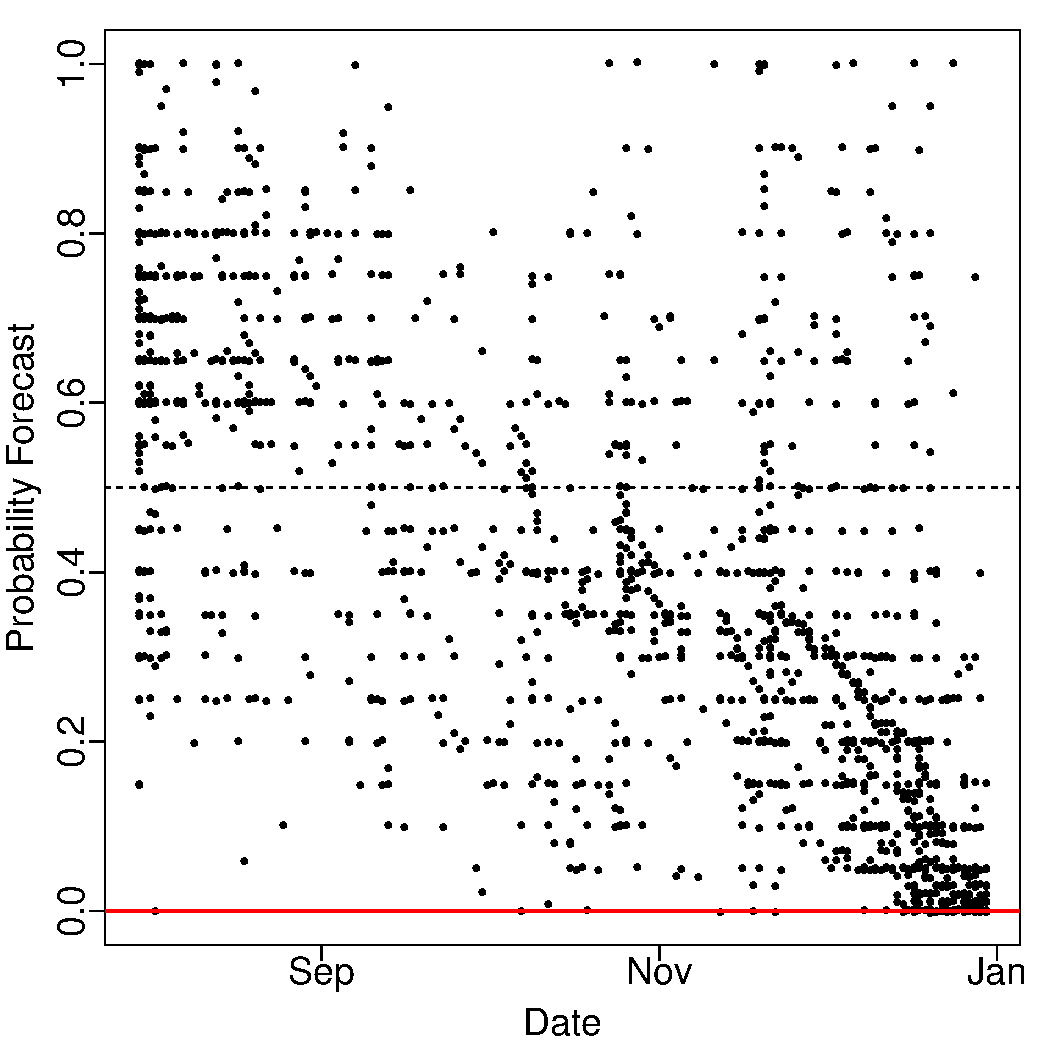
\includegraphics[width=\textwidth]{1127}
                \caption{Probability forecasts of the event ``Will Moody's issue a new downgrade on the long-term ratings for any of the eight major French banks between 30 July 2012 and 31 December 2012?'' The points have been jittered slightly to make overlaps visible.}
                                \label{Example_prob}
\end{minipage}%
\begin{minipage}[t]{.5\textwidth}
%        \end{subfigure}
%        \begin{subfigure}[t]{0.495\textwidth}
                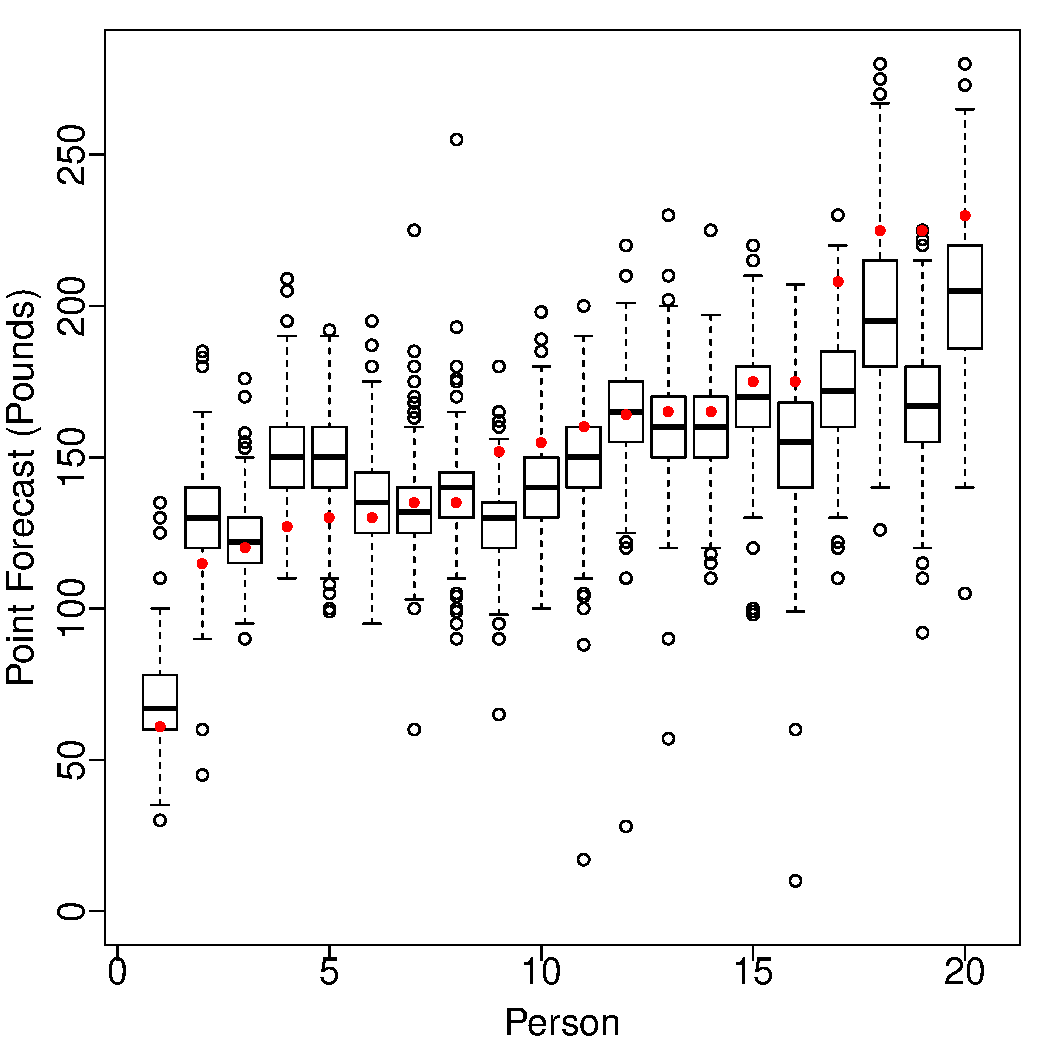
\includegraphics[width=\textwidth]{Weights}
                \caption{Point forecasts of the weights of $20$ different people. The boxplots have been sorted to increase in the true weights (red dots). Some extreme values were omitted for the sake of clarity.}
                                \label{Example_point}
%        \end{subfigure}             
        
%        \caption{Illustration of the real-world forecasts analyzed in this paper. In both subfigures the true values of the target quantities are drawn in red.}
%        \label{Examples}
\end{minipage}%
\end{figure}

We introduce statistical methodology designed specifically for the rapidly growing practice of prediction polling. The methods are illustrated on real-world data involving two common types of responses, namely probability and point forecasts. The probability forecasts were collected 
%during a forecasting tournament that the Intelligence Advanced Research Projects Activity (IARPA) initiated in 2011 as means to estimate the likelihoods of future international political events. Among the participating teams,
by the Good Judgment Project (GJP) (\citealt{ungar2012good, mellers2014psychological}) as a means to estimate the likelihoods of international political future events deemed important by the Intelligence Advanced Research Projects Activity (IARPA). 
%has emerged as the clear winner. 
%% This success is largely credited to the
%%Its strategy 
%has relied on large-scale prediction polling, involving 
%thousands of forecasters making probability estimates
%from professional societies, research centers, alumni associations, science bloggers, and word of mouth. 
%Requirements included at least a Bachelor's degree and completion of psychological and political tests that took roughly two hours. These measures assessed cognitive styles, cognitive abilities, personality traits, political attitudes, and real-world knowledge. 
%Over a period of time these forecasters were then asked to estimate 
% of the events specified by IARPA. These forecasters were allowed to
Since its initiation in 2011, the project has recruited thousands of forecasters to make probability estimates and update them whenever they felt the likelihoods had changed. To illustrate, Figure \ref{Example_prob} shows the forecasts for one of these events. This example involves $522$ forecasters making a total of $1,669$ predictions between 30 July 2012 and 30 December 2012 when the event finally resolved as ``No'' (represented by the red line at $0.0$). 
% ``Will Moody's issue a new downgrade on the long-term ratings for any of the eight major French banks between 30 July 2012 and 31 December 2012?'' and ``Will the Palestinian group Islamic Jihad significantly violate its cease-fire with Israel before 30 September 2012?".
In general, the forecasters reported updates very infrequently. Furthermore, not all forecasters made probability estimates for all the events, making the dataset very sparse. The point forecasts for our second application, on the other hand, were collected by \cite{moore2008use} who recruited $416$ undergraduates from Carnegie Mellon University to guess the weights of $20$ people based on a series of pictures. This is an experimental setup where each participant was required to respond to all the questions, leading to a fully completed dataset. The responses are illustrated in Figure \ref{Example_point} that shows the boxplots of the guesses across forecasters for each of the $20$ people. The red dots represent the corresponding true weights.

%Each question has a timeframe during which the participating forecasters made and updated their estimates as frequently as they liked without penalty. For instance, the question in Figure \ref{Example1} has a timeframe of $154$ days, ranging from 30 July 2012  to 31 December 2012. In general, the forecasters updated their estimates very infrequently, making the dataset extremely sparse. 


%\begin{figure}[t!]
%	\captionsetup[subfigure]{width=0.98\textwidth }
%        \centering
%        \begin{subfigure}{0.495\textwidth}
%                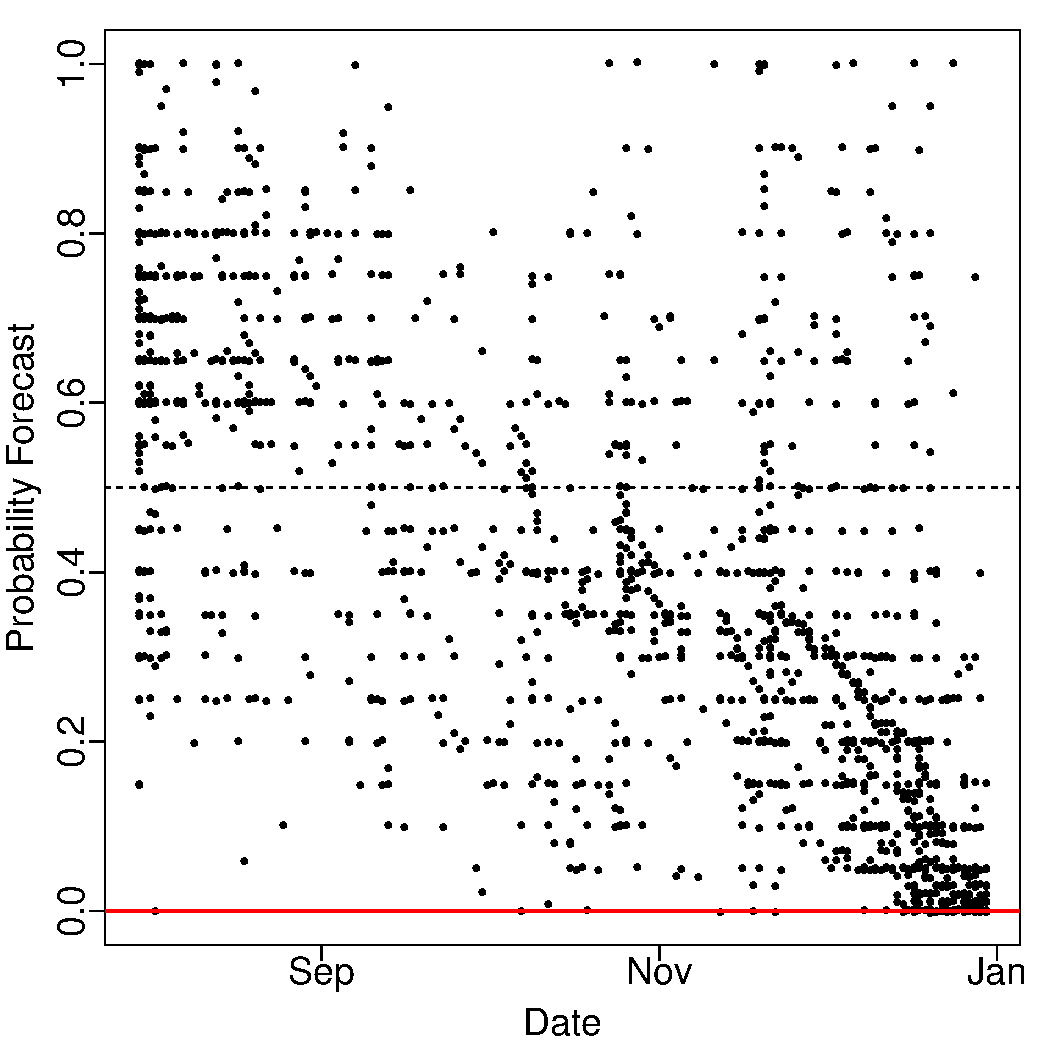
\includegraphics[width=\textwidth]{1127}
%                \subcaption{Will Moody's issue a new downgrade on the long-term ratings for any of the eight major French banks between 30 July 2012 and 31 December 2012?}
%                                \label{Example1}
%        \end{subfigure}
%        \begin{subfigure}{0.495\textwidth}
%                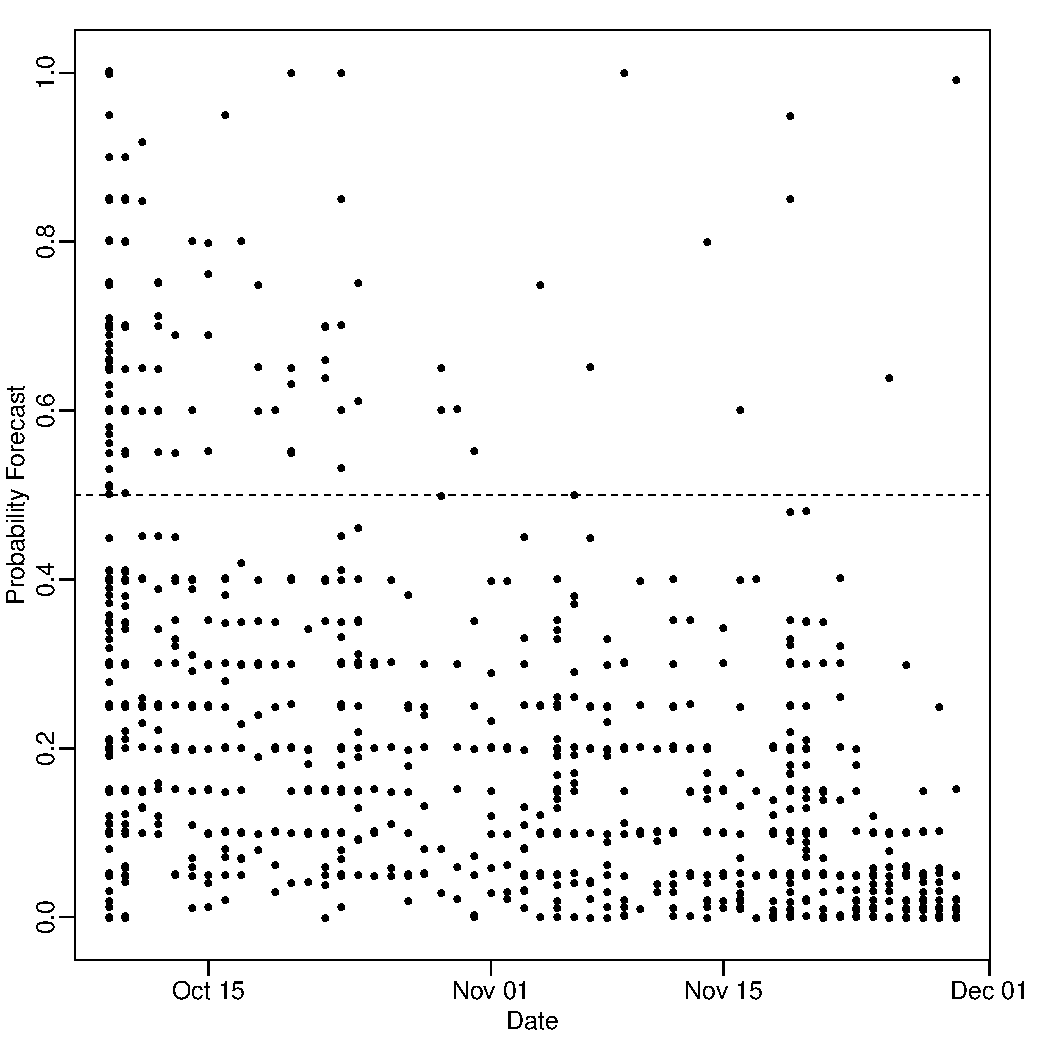
\includegraphics[width=\textwidth]{1160}
%                \subcaption{Will the Palestinian group Islamic Jihad significantly violate its cease-fire with Israel before 30 September 2012?}
%                                \label{Example2}
%        \end{subfigure}             
%        
%        \caption{Two example problems. Given that neither event occurred, the forecasts converge towards the correct answer as the resolution day (the right most point) approaches. Problem (a) involved 522 forecasters, each making, on average, $6.4$ predictions. Problem (b), on the other hand, involved 521 forecasters with an average of $2.1$ predictions per forecaster. The points have been jittered slightly to make overlapping estimates visible.}
%        \label{Examples}
%\end{figure}







%The success of the GJP can be largely credited to its extensive \textit{prediction polling}. This form of polling differs from the more classical \textit{opinion polling} sometimes in a subtle manner and is hence best described with a simple example: Consider a presidential election poll. An opinion poll typically asks the voters who they will vote for. A prediction poll, on the other hand, could ask which candidate they think will win in their state. A liberal voter in a dominantly conservative state is likely to answer differently to these two questions. In broader terms, whereas an opinion poll is a survey of public opinion, prediction poll refers to a setup where multiple agents are collectively predicting the value of some quantity of interest. Prediction polling is, of course, not limited to probability forecasts but can be applied to others types, such as point estimates or even probability density functions, as well. Recently a large number of prediction polls of different types have emerged possibly because modern social and computer networks permit the collection of a large number of responses from a diverse set of sources, including both human or machine agents. This has given rise to crowdsourcing platforms, such as MTurk and Witkey, and many companies, such as Myriada, Lumenogic, and Inkling, that have managed to successfully  capitalize on the benefits of collective wisdom. 



Once the predictions have been collected, the challenge is to combine them into a single consensus. This is typically done for the sake of decision-making and improved accuracy. Principled aggregation, however, requires an assumption about the source of heterogeneity among the forecasts. In particular, it is necessary to specify how the forecasts differ from the true value of the target quantity. For the past several decades, potentially due to the early forms of data collection, measurement error was considered as the main source of heterogeneity. This approach has become the standard and is often applied in practice even when data variation is dominated  by causes besides error in measurement. For instance, assuming measurement error may be reasonable in modeling repeated estimates from a single instrument. However, it is unlikely to hold in prediction polling, where the estimates arise from multiple, often widely different sources. 

%In such setups, the agents' cognitive or information diversity is often more important. 






%These predictions can be point estimates or full distributions that also express the forecaster's degree of uncertainty. 
%Given that information diversity is most likely to be present among collective predictions, the primary focus of this paper is on modeling estimates from a prediction poll. 




%This paper focuses on the development of a theoretical approach to forecast aggregation. The main difference among existing theoretical frameworks is in the assumptions they make about the source of forecast heterogeneity. 

%%the data does not involve repeated measurements.
%% error itself may not make sense at the microlevel. 
% For instance,
% % This boom is particularly attested by the rise of companies such as Myariada, Lumenogic, and Inkling that have successfully  capitalized on the gains of collective wisdom. 
% When modeling such collective forecasts, heterogeneity
%stemming from agents' cognitive or information diversity is often more important than measurement noise. 
%








%Probability forecasting is the science of giving probability estimates for future events. Typically more than one different forecast is available on the same event. Instead of trying to guess which prediction is the most accurate, the predictions should be combined into a single consensus forecast \citep{armstrong2}. This has been 


%
%Forecast aggregation is the problem of combining multiple different forecast into a single forecast with optimal properties. Given that there is strong empirical evidence that an aggregate forecast tends to be more accurate than the individual forecasts \citep{armstrong2}, the practice has spread to a large number of areas, including meteorology \citep{murphy1977reliability}, estimation of inflation and GDP growth \citep{kapetanios2008forecast}, medical diagnosis  \citep{pepe2003statistical}, and predicting geopolitical events \citep{tetlock2005expert}.
%%, estimating future stock prices (Myriada, a finance start-up in London), or prediction markets (Lumenogic; Inkling).  
%Unfortunately, forecasts can be combined in many different ways, and the choice of the combination
%rule can largely determine the predictive quality of the final
%aggregate.  

%
%Forecast aggregation is the problem of combining multiple forecasts into a single forecast with optimal properties. Given that there is strong empirical evidence that an aggregate forecast tends to be more accurate than the individual forecasts \citep{armstrong2}, the practice has spread to a large number of areas, including meteorology \citep{murphy1977reliability}, estimation of inflation and GDP growth \citep{kapetanios2008forecast}, medical diagnosis  \citep{pepe2003statistical}, and predicting geopolitical events \citep{tetlock2005expert}.
%%, estimating future stock prices (Myriada, a finance start-up in London), or prediction markets (Lumenogic; Inkling).  
%Unfortunately, forecasts can be combined in many different ways, and the choice of the combination
%rule can largely determine the predictive quality of the final
%aggregate.  

%There are two general approaches to forecast aggregation: empirical
%and theoretical.  The empirical approach is akin to machine
%learning. Given a training set with multiple forecasts with
%known outcomes, the decision-maker experiments with different
%aggregation techniques and chooses the one that yields the best performance on the training set.
%The theoretical approach, on the other hand, first constructs a
%probability model and then computes the optimal aggregation procedure
%under the assumptions of the model.  This may involve estimating model
%parameters from the forecasts. Both of these approaches are important.  Theory-based procedures that do not
%perform well in practice are ultimately of limited use.  On the other
%hand, an empirical approach without theoretical underpinnings lacks
%both credibility (why should we believe it?)  and guidance (in which
%direction can we look for improvement?). 




%This paper proposes a new source of heterogeneity called the \textit{information diversity}. 
The main contribution of this paper is a new source of forecast heterogeneity, called \textit{information diversity}, that serves as an alternative to measurement error. In particular,  any variation in the forecasts is assumed to stem from information available to the forecasters and how they decide to use it. For instance, forecasters studying the same (or different) articles about a company may use separate parts of the information and hence report differing predictions on the company's future revenue. Such diversity forms the basis of a novel modeling framework known as the \textit{partial information framework}. Theory behind this framework was originally introduced for probability forecasts by \cite{satopaamodeling}; though their specification is somewhat restrictive for empirical applications. We generalize this framework beyond probability forecast and remove all unnecessary assumptions, leading to a new specification that is more appropriate for practical applications. This allows the decision-maker to build context-specific models and aggregators, instead of relying on the usual mean or median aggregates.




%The resulting framework, named the \textit{partial information framework}, is quite flexible yet intuitive.

%This is illustrated by deriving specific partial information models for several different types of forecasts, including point  and probability estimates. 
%These aggregators depend on an information structure for which an efficient estimation procedure is provided. The model is evaluated on several real world forecasting datasets. 


%\marginpar{Focus more on the big picture: this is a new source of heterogeneity which makes much more sense in the prediction context. }


%hat serves as an alternative to measurement error when modeling different forecasts
% This paper proposes a new source of heterogeneity: information diversity. This seems more reasonable at the microlevel when the estimates do arise from different sources. Two contributions: a) the PIF was introduced strictly for probability forecasts in (cite). This paper generalizes the partial information framework beyond probability forecasts; and b) discuss and illustrate estimation both on synthetic and real-world data. 




% PAST: Decades ago statistics was largely geared at data arising from different measurements. This gave rise to the measurement error model, which has been ever since adopted to a wide variety of contexts. Sometimes even when not appropriate. Assigning everything to measurement error, however, does not always seem to follow intuition. For instance, what if there isn't just one measuring device making multiple measurements?
%
% FUTURE: Instead we often have multiple devices making different estimates. Estimates from diverse sources is becoming more prevalent in today's information era. Broad set of applications where this kind of data appears (see Parunak et al. for this).  Can we find a news article that would announce this prevalence? 



%This distinction has a crucial impact on statistical estimation and hence on the applicability of the framework. Given that it is not clear how cognitive diversity can be quantified in theory or measured in practice, reducing the interpreted signal framework to a well-characterized mechanism discoverable through a statistical model seems challenging. The interpreted signal framework is a behavioral model that is realistic yet limited to hypothetical settings where each agent's understanding of reality is known. 


%\subsection{Organization of the Paper}
The paper is structured as follows. Section \ref{PIF} first describes the partial information framework at its most general level and then introduces a practical specification of the framework. 
%This specification culminates in a distribution that describes information diversity with a covariance matrix. 
The section ends with a brief review of previous work on modeling forecasts. Section \ref{estimator} derives a numerical procedure that efficiently estimates the information structure among the forecasters. Section \ref{empirical} illustrates the framework on synthetic and real-world forecasts of different types of outcomes. In particular, the framework is used to analyze probability and point forecasts from the two real-world prediction polls discussed above. The resulting partial information aggregators achieve a noticeable performance improvement over the common measurement-error-based aggregators, suggesting that  information diversity is the more important  source of forecast heterogeneity. 
 Finally, Section \ref{discussion} concludes with a summary and discussion of
future research.



%For instance, consider a group of forecasters making independent predictions of a company's future revenue. The team members  may vary largely in terms of skill and knowledge. 
%\subsubsection{Bayesian Framework}
%
%
%\marginpar{Must read this paper and explain it. This might have to be in the interpreted framework.}

%\subsection{Empirical Approaches}
%If one is not concerned with theoretical justification, an obvious
%approach is to perturb a simple aggregator and observe whether the
%adjusted estimator performs better on some data set of interest.  
%%Given that the measurement error
%%framework produces under-confident aggregators, a popular adjustment is to {\em extremize}, that is, to shift the average aggregates closer to the
%%nearest extreme (either zero or one) (see, e.g.,  \citet{Ranjan08, satopaa, mellers2014psychological}). 
%Such approaches, however, do not reflect an actual model of forecasts and require a training set with known outcomes. Given that this paper does not assume known outcomes, empirical techniques are not discussed further. 


%Any linear opinion pool of calibrated forecasts, however, is today known to be both uncalibrated and under-confident \citep{Ranjan08}.

%Some preliminary steps have been made towards a more concrete model by, for example, assuming
%conditional independence of the $x_i$, \cite{}, but
%lacking a distributional model. 

%To the best of our knowledge, no previous work has discussed a formal framework that explicitly links the interpreted forecasts to their target quantity. Consequently, the interpreted signal framework, as proposed, has remained relatively abstract. 
%%The interpreted signal framework, when formalized, more or less implies the partial information framework.
%%The present paper, however, formalizes the intuition behind it. 
%%The interpreted signal framework, when formalized, more or less implies the partial information framework. 
%The partial information framework, however, formalizes the intuition behind it, allows quantitative predictions, and provides a flexible construction that can be adopted to a broad range of forecasting setups. 


%\section{Motivating Applications and Forecasting Data}
%\label{examples}
%Information diversity appears among many facets of real-world applications. This paper use the partial information models to analyze real-world probability forecasts of geopolitical events and [OTHER APPLICATION]. These models are sensitive to the structure of the
%information overlap that is assumed to hold among the individual
%forecasters. Model sensitivity is useful if it reacts
%to important inherent features of the problem, but harmful if it adds
%noise that is not reflected in the actual best response to the data.
%It therefore behooves us to begin with some simple examples to show
%that the optimal aggregate estimate is not well defined without
%assumptions on the information structure among the forecasters. 
%
%\begin{example}[Exchange Rates]
%Consider two forecasters who aim to predict the one-year percentage change in the EUR/USD exchange rate. Suppose both forecasters report $+10\%$. If they are seeing the same evidence, then the optimal aggregate
%forecast is $+10\%$.  If they are seeing different evidence, then clearly the combined evidence should give an aggregate forecast somewhat greater than $+10\%$. 
%\end{example}
%
%
%\marginpar{Describe the ideal context: investors making bets on the change of a daily stock market. Eventually their estimates can be calibrated. Furthermore, we can run a estimate the information structure. }
%
%\marginpar{May not need these examples. Might be more interesting to focus on the broad range of applications where this kind of data apply. LETS MAKE THIS AN APPLICATION DRIVEN PAPER. In order for this paper to get into the application faster, we should introduce the datasets here in more detail. That will really give it the right feel. }
%
%\marginpar{May also want to discuss why calibration is necessary, that we calibrate our data before hand; we cannot simply use naive forecasters. Some quality control is needed.}
%
%%\begin{example}[Real Estate Valuation]
%%Suppose  a number of descriptions (or a lengthy) description of a house for sale, one would want to add of the different contributions to the overall value of the house (a garage, a deck, new kitchen appliances), but to downweight
%%repeated descriptions of the same thing (e.g. redundant talk about how good condition the house is in, or redundant expressions of the quality of the neighborhood).
%%\end{example}
%
%\begin{example}[Sports] 
%\label{sports}
%Suppose the final score of a baseball game depends only on the teams' defensive and offensive qualities. Three spectators make predictions about the final score. The first two only consider the teams' defensive qualities and report respective predictions of $8$-$2$ and $4$-$0$. The third spectator, on the other hand, considers only the teams' offensive quality and predicts $0$-$7$. The average of the individual predictions is $4$-$3$. If, however, the defensive and offensive qualities are equally important, a better aggregate forecast is obtained by first averaging the predictions that are based on the same team quality and then averaging these two averages. This gives an aggregate score of $3$-$4$. 
%\end{example}
%
%\marginpar{Cite the other paper for the motivation for all this theory}
%
%%$a_1-b_1$, $a_2-b_2$, $a_3-b_3$
%%
%%\begin{align*}
%%a_1+a_2+a_3 &= 3 A_{ave}\\
%%b_1+b_2+b_3 &= 3 B_{ave}\\
%%a_1+a_2+2a_3 &= 4A_{pif}\\
%%b_1+b_2+2b_3 &= 4B_{pif}\\
%%\\
%%Sa+a_3 &= 3 A_{ave}\\
%%Sb+b_3 &= 3 B_{ave}\\
%%Sa+2a_3 &= 4A_{pif}\\
%%Sb+2b_3 &= 4B_{pif}\\
%%\\
%%Sa &= 2(3A_{ave} - 2 A_{pif})\\
%%Sb &= 2(3B_{ave} - 2B_{pif})\\
%%a &=  4A_{pif} -3 A_{ave}\\
%%b &=  4B_{pif} -3B_{ave}\\
%%\\
%%Sa &= 2(3A_{ave} - 2 A_{pif})\\
%%Sb &= 2(3B_{ave} - 2B_{pif})\\
%%a &=  4A_{pif} -3 A_{ave}\\
%%b &=  4B_{pif} -3B_{ave}\\
%%\end{align*}
%
%
%The purpose of these two preliminary examples is two-fold: a) they illustrate the broad range of applications under which partial information overlap influences aggregation; b) Example \ref{sports} shows how the measurement error framework can lead to misleading aggregation when information among the forecasters is unevenly distributed (as is the case in many real-world applications). The next two examples make more concrete statements by performing detailed computations. 
%
%
%\begin{example}[Discrete Outcome]
%Suppose an experimenter rolls a fair die. Let $Y$ represent the outcome of the roll. Two forecasters aim to predict the value of $Y$.  First, however, each of them gets to observe one of the two events:
%\begin{align*}
%A_1 &= \{Y \in \{1, 3, 5\}\}\\
%A_2 &= \{Y \in \{1, 2, 6\}\}
%%Y &\in \{1, 2, 4, 6\}\\
%%Y &\in \{1, 3, 4, 5\}
%%%%Y &\in \{1, 2, 5, 6\}\\
%%%%Y &\in \{1, 3, 4, 6\}
%\end{align*}
%If the experimenter rolled a one, both forecasters would predict a three. Now, the optimal aggregate depends on the forecasters' information: if they observed the same event, the aggregate is three; but, if they observed different events, the aggregate is one.
%\end{example}
%In this example, it is not possible to distinguish between the two different information structures simply based on the given predictions. If the forecasters had participated in a long sequence of independent replications of the given task, it may have been possible to eventually ascertain whether they have the same information or not. Similarly, if their forecasts had disagreed, it would have been easy to conclude that they did not observe the same event.  However, in the given situation, there
%was no way to know, and neither one nor three can be said to be a
%better choice for the aggregate forecast. 
%%The next example illustrates show that without knowing the information structure, the optimal aggregate forecast of a continuous variable can be anywhere between two different forecasts. 
%%
%%\begin{example}[Continuous Outcome]
%%Consider two forecasters 1 and 2 predicting the value of a random variable $U$ that is uniform over the unit interval $[0,1]$. Define two intervals 
%%\begin{align*}
%%I_1 &= [0.48+\varepsilon, 0.68 - \varepsilon]\\
%%I_2 &= [0.32-\varepsilon, 0.52 + \varepsilon],
%%\end{align*}
%%where $\varepsilon \in [-0.08, 0.08]$. Suppose forecaster $i$ knows that $U \in I_i$. The information overlap varies in $\varepsilon$. In particular, when $\varepsilon = 0$, the events $U \in I_1$ and $U \in I_2$ are independent; hence the forecasters information sets are independent. On the other hand, when $\varepsilon = 0.08$, forecaster 1's information contains forecaster 2's information, making it irrelevant. When  $\varepsilon = -0.08$, the opposite happens. The forecasters' predictions, however, are not affected by the choice of $\varepsilon$. More specifically, forecaster 1 always predicts $\E[U | U \in I_1] = 0.58$ and forecaster 2 predicts $E[U | U \in I_2] = 0.42$. The optimal aggregate $\E[U | U \in I_1 \cap I_2] = 0.5 + \varepsilon \in [0.42, 0.58]$, on the other hand, is affected by this choice. 
%%\end{example}
%The next example shows that even if the forecasters observe independent events, further details
%in the structure of information can still greatly affect the
%optimal aggregate forecast.
%
%\begin{example}[Continuous Outcome]
%Consider two forecasters 1 and 2 predicting the value of a random variable $U$ that is uniform over the unit interval $[0,1]$. Let $\epsilon > 0$ be some small value. Consider the three intervals 
%\begin{align*}
%I_1 &= [0, 1/2]\\
%I_2 &= [1/4-\Delta, 1/2- \Delta]\\
%I_3 &= [\ee + 1/2+ \Delta, \ee + 3/4+ \Delta]
%\end{align*}
%where $\Delta \in [0, 1/4 - \ee]$, and define two events $S_1 = \{ U \in I_1\}$ and $S_2 = \{ U \in I_2 \cup I_3\}$. Consider two forecasters and suppose forecaster $i$ observes $S_i$. Therefore the $i$th forecaster's information set is
%given by the $\sigma$-field $\F_i$ containing $S_i$ and its
%complement. Their $\sigma$-fields are independent.   forecaster~1
%reports $X_1 = 1/4$ if $S_1$ occurs;
%otherwise, $X_1 = 3/4$.  forecaster~2, on the other hand, reports $X_2 = (1+\ee)/2$ if $S_2$ occurs; otherwise, $X_2 = (1-\ee)/2$. Changing $\Delta$ does not affect these forecasts, nor does it
%change the fact that each of the four possible pairs of forecasts has
%probability $1/4$.  Therefore all observables are invariant under
%this perturbation.  If forecasters $1$ and $2$ predict $1/4$ and $(1+\ee)/2$, respectively, then the optimal aggregate forecast is $3/8-\Delta$, which is most
%definitely affected by the perturbation.
%\end{example}
%
%It is not difficult to imagine many more illustrative examples with increasing complexity. These examples, however, suffice to show that the aggregation problem can be largely affected
%by the structure of information overlap.  Therefore, we conclude that the model must  incorporate an assumption as to the structure of the information
%overlap, and that the details must be informed by the particular
%instance of the problem. 
% 
%%
%%Information diversity occurs in nearly every discipline. A number of examples
%%are given here to illustrate the variety of contexts where information diversity 
%%can be present. 
%%\begin{itemize}
%%\item The wisdom of the crowd with an application  to probability forecasting. Be careful here though. It must be a problem where information plays a crucial role in decision making; hence more informed have an advantage. 
%%\item Online rating. Consider, say, Yelp that collects different customers' ratings on a scale from 1 to 5. Customer A may focus entirely on the food in the restaurant. Based on this he is going to give a rating of, say, 3. At this point it is fair to say that his assessment does not reflect the quality of the entire restaurant. Instead, it is only an assessment of a part of it, namely, the food. Yelp, however, would like to have an accurate overall summary of the quality of the restaurant. To make this point more clear, consider a restaurant whose two characteristics are only food and service. Both range in quality from 1 to 5. Their average then gives the overall performance. Say three customers enter: A, B, and C, where A and B rate only the food and C only the service. A, B, and C give ratings of 3, 4, and 5, respectively. Averaging these scores, and hence ignoring the information of the customers, would lead to an overall score of (3+4+5)/3 = 12/3 $\approx$ 4. But this is not an accurate story at all. The assessments target very different aspects of the restaurant. A more appropriate assessment would be to average the aspect specific scores first. That is, a more honest score would be $((3+4)/2 +5)/2 \approx 4.25$. Therefore, in this case, the overall performance of the restaurants would be underestimated by the naive, overall averaging technique. Many similar arguments can be found, and this is really not dependent on the scale being finite. 
%%
%%\item Bayesian statistics and informative prior aggregation. Also, if you have some N probability forecasts from a posterior. How do you aggregate these?
%%\item Online ratings or house sale with extra information. 
%%\item Ensemble learning. Can estimate information structure completely.
%%\item Voting and subtle distinction in survey sampling. Maybe include examples that are NOT.
%%%\item Jury Models
%%%\item electronic markets
%%%\item crowdsourcing applications in general
%%\end{itemize}
%%
%%Explain at the end that this FIRST paper focuses on probabilistic forecasts foe the sake of brevity and provides the cleanest entry to the issues of concern etc.
%%


\section{Partial Information Framework}
\label{PIF}

\subsection{General Framework}
\label{context}



Consider $N$ forecasters and suppose forecaster $j$ predicts $X_j$ for some (random) quantity of interest $Y$. This prediction $X_j$ is simply an estimator of $Y$. Therefore, as is the case with all estimators, 
%If the forecaster operates under the quadratic loss function, the optimal strategy is to report the expected value of $Y$ given all the information 
its deviation from the truth can be broken down into two components: bias and noise. On the
theoretical level, it is important to separate these two problems because they are addressed by different mechanisms.  This
paper considers the aggregation problem for conditionally unbiased forecasts,
therefore isolating the task to one of noise reduction. In particular, the forecasters are assumed to be conditionally unbiased such that $\E[Y | X_j] = X_j$ for all $j = 1, \dots, N$; that is, among all those times that forecaster $j$ predicts $X_j$, the quantity of interest $Y$ is, on average, equal to $X_j$. 
%This is an assumption about the quality of the forecast. In general some form of quality control is needed because no aggregator can be expected to turn nonsensical responses into accurate aggregate forecasts. 
%A stream of conditionally biased forecasts can, in principle, be corrected by
%translating $X_i$ into the forecast $\bar{Y}_i$, where $\bar{Y}_i$ is
%the historical average of the outcomes when $X_i$ is
%forecast.  One can then assume without loss of generality that the
%forecaster is conditionally unbiased, replacing $X_i$ if necessary by the
%historically corrected $\bar{Y}_i$. This assumption is, of course, valid
%only in principle: it relies on a relatively lengthy history and an
%assumption of stationarity of the properties of the forecasts.  
%Nevertheless, 
%
%Before delving into the problem of forecast aggregation, it is useful
%to briefly discuss the problem of assessing and improving a single
%forecast stream.  
This assumption is, to some degree, self-fulfilling if the forecasters operate 
%The forecasters are assumed to operate
 under a 
%Both aggregate and individual forecasts are typically assessed with a loss
%function.
%%$L(X_i, Y)$. 
%Many choices are possible, and
%an estimator that outperforms another under one loss function will not
%necessarily do so under a different one. In this paper  the focus is on l
loss function that is minimized at the conditional expectation of $Y$ (given the forecaster's information). In this paper such loss functions are deemed \textit{revealing}. This group of functions involves many well-known penalties such as the Kullback-Leibler divergence, Mahalanobis distance, and the quadratic loss \citep{banerjee2005optimality}. 
%These loss functions can be considered \textit{revealing} because if a group of
%sophisticated forecasters operates under such a loss function,
%the assumption of conditionally unbiased forecasts is, to some degree,
%self-fulfilling. 

%\marginpar{the model is a bit different as before; negative correlation.}
% forecasters can improve their long run performance via training and active
%feedback. forecasters with competitive
%motivation, sophistication, and historical data will probably do so.


% Secondly, the
%assessment of the aggregated forecast is not uni-dimensional any more
%than is the assessment of an individual forecast.  In order to compare
%different aggregation procedures, a loss function must be chosen.  In
%practice, the quadratic score is the most common choice, perhaps because
%of its simplicity, or because of the
%paramount status of variance in the statistical literature. This paper concentrates on minimizing the variance of the aggregators, though
% much of the discussion holds under general loss
%functions.




%The partial information framework was originally introduced for probability forecasts in \cite{satopaamodeling}. This section elaborates and generalizes the framework beyond probability forecasts. Even though much of the discussion and motivation given in \cite{satopaamodeling} carries directly over, the overlap in content is kept at minimum. 

\marginpar{This needs work but should talk to Robin first}

%The construction  of the partial information framework begins with
%Consider
The partial information framework assumes that the observables $Y$ and $X_j$ are measurable random variables under some probability space $(\Omega, \F , \P)$.  The probability measure $\P$ provides a non-informative (proper) prior on $Y$ and  reflects the \textit{basic information} known to all forecasters. 
%There is one substantive
%assumption in this model, namely the choice of the prior distribution $\P(Y)$. Given that this prior serves as a reference point for estimating levels of forecaster information, it should be both proper and non-informative. 
Such a prior has been discussed extensively in the economics and game theory literature where it is usually known as the \textit{common prior}. 
%(see, e.g., \citealt{morris1995common, dawid1995coherent}). 
Even though this is a substantive assumption in the framework, specifying a prior distribution cannot be avoided as
long as the model depends on a probability space. This includes essentially any probability
model for forecast aggregation. How the prior is incorporated depends on the problem context: it can be chosen explicitly by the decision-maker, computed based on past observations of $Y$, or estimated directly from the forecasts. 

%\marginpar{As we will see in some cases we can in fact estimate this prior; hence produce an aggregator with no tuning parameters.}



The principal $\sigma$-field $\F$ can be interpreted as all the possible information that can be known about $Y$. Under the partial information framework, the forecasters operate under the same probability model but use different subsets of the full information. In fact, in any Bayesian setup, with a revealing loss function, it is more or less tautological that
%More specifically,
forecaster $j$ predicts $X_j = \E[Y \| \F_j]$ based on some partial information $\F_j \subseteq \F$. Therefore $\F_i \neq \F_j$ if $X_i \neq X_j$ such that forecast heterogeneity stems purely from \textit{information diversity}. 
%, where $\F_j \subseteq \F$ is
% the \textit{information set} used by the forecaster.
 Note that forecaster $j$ may have access to some larger $\sigma$-field $\G$ but only decides to use $\F_j \subseteq \G$. For the purposes of aggregation, however, any available information discarded by the forecaster may as well not exist. Therefore the \textit{information set} $\F_j$ is defined explicitly as the information used by the forecaster. 
 Overall, this is not in any way restrictive. In fact, by letting $\F_j = \sigma(X_j)$ be the $\sigma$-field generated by $X_j$, the forecasts can be written as $ \E[Y \| \F_j] =  \E[Y \| X_j] = X_j$, which suggests nothing but the conditional unbiasedness property discussed in the previous section together with the existence of an underlying probability model. 
 % based on different information sets. 
%To see that this assumption is not in any way restrictive, recall that a conditionally unbiased forecaster predicts $\E [Y \| X_j] = X_j$. Under the given probability model, conditioning on $X_j$ is equivalent to conditioning on $\sigma(X_j) = \F_j$, namely the smallest $\sigma$-field generated by $X_j$, and hence $\E [Y \| X_j] =  \E [Y \| \F_j] = X_j$. Consequently, the assumption
% $X_j = \E [Y | \F_j]$ only requires the existence of a probability model, together with the assumption of conditional unbiasedness. 
 
 
 This is enough to provide the following proposition that relates the target quantity to the forecasts. The proof is deferred to the Appendix.
 \begin{proposition}
\label{covstr}
Suppose $\E[Y|X_j]  = X_j$ for all $j =1, \dots, N$. Denote $\F_j = \sigma(X_j)$ and consider a sub-$\sigma$-field $\sigma(X_i) = \F_i \subseteq \F_j$ for some other forecast $X_i$. Then,
\begin{enumerate}[i)] 
\item $\E[Y] = \E[X_j]$ for all $j = 1, \dots, N$, \label{first}
\item $\Cov(X_j, X_i) = \Var(X_i)$, and  \label{second}
\item $\Var(X_i) \leq \Var(X_j)$.  \label{third}
\end{enumerate}
\end{proposition}
\noindent
Item \ref{first}) states that the target quantity and the forecasts agree in expectation. This is particularly useful as it provides guidance in estimating the prior of $Y$. 
% This suggests that  if the $X_j$'s are probabilistic (such as densities), the prior distribution $\P(Y)$ can be estimated from the forecasts. On the other hand, if $X_j$ are point estimates, the prior mean $\E[Y]$ can be estimated from the $X_j$'s. 
%
%This suggests that all the relevant model parameters can be estimated in practice.
%Furthermore, given that $X''$ and the $X_j$'s have the same support, the choice of $\delta_0$ is irrelevant when the $X_j$'s are point estimates. On the other hand, if the $X_j$'s are probabilistic (such as densities), $\delta_0$ can be estimated from them by referring to item \ref{first}) of Proposition \ref{covstr}.  For convenience and without loss of generality, the rest of the paper assumes that the link function performs scaling such that $\delta_0 = 1$ in (\ref{NExperts}).  
Given that $Y = \E[Y | \F]$ and $\F_j \subseteq \F$ for all $j = 1, \dots, N$, item \ref{second}) shows that the covariance matrix $\bSigma_X$ of the $X_j$'s extends to the unknown $Y$ as follows:
\begin{align}
\Cov\left((Y, X_1, \dots, X_N)'\right) &=  \left( \begin{matrix} 
 \Var(Y)  & \diag(\bSigma_X)'  \\
\diag(\bSigma_X) & \bSigma_X \\
\end{matrix} \right), \label{cov_str}
\end{align}
where $\diag(\bSigma_X)$ denotes the diagonal of $\bSigma_X$.
%
% $\Cov(X_j, Y) = \Var(X_j)$ because $Y = \E[Y | \F]$ and $\F_j \subseteq \F$ for all $j = 1, \dots, N$.
%  This explains how the covariance matrix of the observables, namely the $X_j$'s extends to the unknown $Y$ (see Equation (\ref{NExperts})).
This allows $Y$ to be regressed on the $X_j$'s without a separate training set of past predictions and known outcomes. The resulting estimator, called the \textit{revealed} aggregator, is denoted with $X'' := \E [Y \|
\F'']$, where $\F'' := \sigma(X_1, \dots, X_N)$ is the $\sigma$-field generated (or revealed) by the forecasts
$\{X_j : j = 1, \dots, N \}$. The revealed aggregator optimally utilizes the information in the forecasts and is therefore the relevant estimator in each specific partial information model. Finally, item \ref{third}) shows that $\Var(X_j)$ increases to $\Var(Y)$ as forecaster $j$  learns and becomes more informed about $Y$. Therefore $\Var(Y)$ is the total amount of available information and $\Var(X_j)$ is the amount of information used by forecaster $j$. 
%and $\Var(X_j)$ quantify the amount of information in $\F$ and $\F_j$, respectively.  
%represents the total amount of information and $\Var(X_j)$ is the amount of information used by forecaster $j$.
 Consequently, $\Cov (X_{i} , X_{j})$ can be viewed as the amount of information overlap between forecasters $i$ and
$j$. 
%These variables are collected in the sub-matrix $\bSigma$ that represents the \textit{information structure} among the $N$ forecasters. 



%\marginpar{Discussion of item i should be place here. Keep it as one in the following text.}

% Together these observations  
%This arises directly from the existence of a probability model and the assumption of calibration because for a calibrated forecaster, $\E(\one_A | p) = p$, which shows constructively that $p$ is of the form $\E(A | \G)$ for some $\G$. 
%The
%partial information framework extends this idea to $N$
%forecasters. 


%\marginpar{Here P is the noninframtive prior; must be proper. }

%The information sets contain the basic information plus any additional information actually used by the
%forecasters. To make this more precise, suppose forecaster $j$ has access to the information in a sub-$\sigma$-field $\G \subseteq \F$. Any forecast that is measurable with respect to $\G$ is then a valid prediction for forecaster $j$. The actual forecast, however, does not necessarily have to be $\E[Y | \G]$ but rather $\E[Y | \F_j]$ for some $\F_j \subseteq \G$. Therefore the available information and the information actually used may not be the same.
%% if forecaster $i$ uses a simple rule, the set $\F_i$ may not be the full $\sigma$-field of
%%information available to the forecaster but rather a smaller
%%$\sigma$-field corresponding to the information used by the
%%rule.  For example, when forecasting the future price of a stock,  a forecaster obeying the dictum ``it's the economy,
%%stupid!''  might utilize a $\sigma$-field containing only economic
%%indicators.
% Furthermore, if two forecasters have access to the same $\sigma$-field, they may decide to use different sub-$\sigma$-fields, leading to different predictions. 
%%This is reminiscent of a forecasting algorithm that only uses
%%a similarly restricted subset of information. 
%Therefore,
%forecast heterogeneity does not only stem from differences in the available information, but also from how the forecasters decide to use it.  Note, however, that if a forecaster chooses to discard
%some of the available information, then, for the purposes of aggregation,
%that information may as well not exist. 
%%Therefore, for the sake of clarity, from now on $\F_i$ can be referred to simply as the information known to forecaster $i$.
%

%Overall, the partial information framework is quite flexible
%yet intuitive. In fact, it is not difficult to imagine a variety
%of other forecasting setups and how they translate to
%different inter-dependencies among the information sets.
%%Any further details must come from the
%%assumptions on the structure of the information sets. To illustrate, 
%For instance, suppose that the forecasters are asked to predict a sequence of values
%$\{Y_1, Y_2 , \ldots \}$. The framework only assumes that
%forecaster~$j$ uses some $\sigma$-field $\F_{jk}$ to make a forecast for $Y_k$.  Further aspects of the problem
%are reflected by the structure of the collection $\{ \F_{jk} \}$.  For
%example, if the values are sequenced in time, then the information
%sets $\{ \F_{jk} : k = 1 , 2, 3, \ldots \}$ are likely to form an
%increasing sequence.  If the forecasts are public, it is reasonable 
%to assume that $\F_{jk}$ contains all forecasts up to time $k-1$.
%If, in addition, the forecasts of each individual event $A_j$ are sequenced rather %than synchronous, the set $\F_{ij}$ may contain information about %some forecasts at time $j$ as well.  

%
%
%The partial information framework distinguishes two benchmarks for aggregation efficiency.  The first is the {\em oracular} aggregator
%$X' := \E [Y \| \F']$, where $\F'$ is the $\sigma$-field
%generated by the union of the information sets $\{\F_j : j = 1, \dots, N\}$.  Given that aggregation cannot be improved beyond using all the information  of the forecasters, the oracular aggregator represents a theoretical optimum in estimation efficiency.  In practice, however, information comes to the
%aggregator only through the forecasts $\{X_j : j = 1, \dots, N\}$. Given that $\F'$ generally cannot be constructed from these forecasts alone, no practically feasible aggregator can be expected to perform as well as $X'$. Therefore $X'$ is only useful in theoretical analysis and is therefore not discussed further in this paper. For more information see \cite{satopaamodeling} that uses the oracular aggregator to analyze the empirical technique of extremizing, i.e., shifting an average aggregator closer to the nearer extreme (zero or one). A more achievable benchmark is the \textit{revealed} aggregator $X'' := \E [Y \|
%\F'']$, where $\F''$ is the $\sigma$-field generated (or revealed) by the forecasts
%$\{X_j : j = 1, \dots, N \}$. Given that this benchmark can be applied in practice, it is the relevant estimator in each specific partial information model. 
%













%\subsection{Information Abstraction}
%In practice, it is unlikely that the information sets $\mathcal{F}_j$  can ever be known with fine precision.  Therefore it is necessary to make reasonable assumptions that yield plausible yet generic information structures. To abstract the forecasters' information, a natural first step is to only consider the amount of information used by a forecaster and the size of the information overlap among the forecasters. 
%
%\marginpar{This needs to be shortened; somehow condense this section, it is too long.}
%
%The former quantity can be estimated by comparing a forecast with the non-informative forecast. More specifically, forecaster $i$ with no information reports a non-informative prediction given by the prior expectation; that is, if $\mathcal{F}_i =\{\emptyset, \Omega\}$, then $X_i = \E(Y)$. On the other hand, if forecaster $i$ uses all the information,  $X_i$ is a point mass at the correct value of $Y$; that is, if $\mathcal{F}_i = \mathcal{F}$, then $X_i = \E(Y|\mathcal{F}) = Y$.  These logical extremes characterize the forecasters' behavior at different levels of information, and the distance to the non-informative forecast facilitates estimation of the forecaster's amount of information. 
%
%Estimation of the latter quantity, on the other hand, relies on the correlation of the forecasts. To make this more specific, recall that two $\sigma$-algebras $\mathcal{F}_i$ and  $\mathcal{F}_j$ are called independent if for all $B \in \mathcal{F}_i$ and $C \in \mathcal{F}_j$ the events $B$ and $C$ are independent, i.e. $\P(B \cap C) = \P(B) \P(C)$. In other words, $\mathcal{F}_i$ does not provide any additional information about $\mathcal{F}_j$, and \textit{vice versa}. Therefore independent $\sigma$-fields can be considered \textit{informationally disjoint}. Given that $X_j$ is measurable with respect to $\mathcal{F}_j$,  forecasts based on informationally disjoint sets are independent and hence uncorrelated. At the other extreme, if $\mathcal{F}_i = \mathcal{F}_j$, the forecasts $X_i$ and $X_j$ are the same and have a perfect positive correlation.  Therefore it is reasonable to assume that the correlation between any two forecasts increases in size of the forecasters' information overlap. 
 
% \subsection{Interpretation}
% Explain the covariance structure and show how it can be interrupted. 
% 

\subsection{Gaussian Partial Information Model}
\label{gaussian}
The general partial information framework is clearly too abstract to be applied in practice. A more specific model within the framework is needed. The first step is to choose a joint distribution for the model variables $Y, X_1, \dots, X_N$. This in general requires an understanding of how the model variables change together. A natural solution refers to Proposition \ref{covstr} and parametrizes the joint distribution in terms of covariances. This points towards a multivariate Gaussian distribution, which is a typical starting point in developing statistical methodology. Furthermore, the conditional distributions of a multivariate Gaussian distribution  have simple forms also within the Gaussian family. This turns out to be particularly useful in deriving the revealed aggregator. 
%Furthermore, it has  

% Second, both the multivariate and conditional Gaussian distributions are well-studied and have simple forms. 
%This is especially useful in deriving the revealed aggregator.   



%has the additional benefit of providing easy access to the revealed aggregator $X'' = \E[Y|X_1, \dots, X_N]$. 
%In particular, if $Y, X_1, \dots, X_N$ follow a multivariate Gaussian distribution, then $Y|X_1, \dots, X_N$ is a also Gaussian with simple well-known forms for the mean and variance parameters.


%Furthermore, given that the main task is to predict $Y$ from the $X_j$'s, the chosen distribution should also facilitate easy derivation of the revealed aggregator $X'' = \E[Y|X_1, \dots, X_N]$. Both of these requirements point towards a multivariate Gaussian distribution. 

From the intuitive point of view, the choice of the Gaussian distribution can be motivated by the model discussed in \citet{broomell2009experts}. 
%They discuss a model in which 
They assume that
% recall the interpreted signal
%model of~\citet{broomell2009experts}. They assume that
forecaster~$j$ forms an opinion based on a linear function $L_j$ of cues
$H_1 , \ldots , H_M$.
% influencing $Y$.  
%Proposing a linear model for subjective
%interpretation seems quite natural.  
If
the cues (or any linear combination of them) are independent
and have small tails, then as $M \to \infty$, the joint distribution
of the linear combinations $L_1 , \ldots , L_N$ will be asymptotically
Gaussian.  Therefore, given that the number of cues in a real-world setup is likely to be large, it makes sense
to model the forecasters' observations as jointly Gaussian. 

\marginpar{Mathematically tractable. See Many testing, estimation and confidence interval procedures discussed in the multivariate
statistical literature are based on the assumption that the observation vectors
are independent and normally distributed (Anderson, 2003, Srivastava and Khatri, 1979,
Muirhead, 1982). There are two main reasons for this. Firstly, sets of multivariate observations
are often, at least approximately, normally distributed. Secondly, the multivariate
normal distribution is mathematically tractable. Normally distributed data can be modeled
entirely in terms of their means and variances/covariances. Estimating the mean and
the covariance matrix are therefore problems of great interest in statistics, as well as in
many related more applied areas. From Studies in Estimation of Patterned Covariance Matrics -- Martin Ohlson}

Unfortunately, in many setups $Y$ and $X_j$ may not be real-valued. For instance, in probability forecasting of binary events, it is common to let $Y \in \{0,1\}$ and $X_j \in [0,1]$. This limitation, however, can be handled by borrowing from the theory of generalized linear models \citep{mccullagh1989generalized} and utilizing a \textit{link function}. To make this concrete, consider $N+1$ auxiliary variables, called the \textit{information variables}, that follow a multivariate Gaussian distribution with the covariance pattern (\ref{cov_str}):
\begin{align}
\left(\begin{matrix} Z_Y \\ Z_{1}\\ \vdots \\ Z_{N} \end{matrix}\right) &\sim \mathcal{N}_{N+1}\left( 
%\left(\begin{matrix} 
%\mu_1 \\ \boldsymbol{\mu}_2
% \end{matrix}\right) =
 \boldsymbol{0}, \left(\begin{matrix} 
1 & \diag(\bSigma)'\\
\diag(\bSigma) &\bSigma\\
 \end{matrix}\right) 
 :=
 \left(\begin{array}{c | c c cc }
1 & \delta_1 & \delta_2 & \dots & \delta_N  \\ \hline
\delta_1 & \delta_1 &\rho_{1,2} & \dots & \rho_{1,N}   \\ 
\delta_2 & \rho_{2,1} & \delta_2 & \dots & \rho_{2,N}  \\ 
\vdots & \vdots & \vdots & \ddots & \vdots  \\ 
\delta_N & \rho_{N,1} & \rho_{N,2} & \dots & \delta_N\\ 
 \end{array}\right)\right).  \label{NExperts}
\end{align}
%Practical application of the revealed aggregator $X'' = \E[Y|X_1, \dots, X_N]$ begins with an understanding of how $Y$ and $X_j$ change together.  Therefore 
%A practical specification of the partial information framework begins with a joint probability distribution for the model variables. Any distribution can be used as long as it can utilize the covariance pattern in (\ref{cov_str}) and permits estimation of $Y$ given the $X_j$'s.  However, directly stating such a joint distribution in some applications, such as probability forecasting of binary events, can be difficult because $Y$ and $X_j$ may not share a common support. This can be generally addressed by introducing $N+1$ auxiliary \textit{information variables} denoted with $Z_Y, Z_1, \dots, Z_N$. Let their joint distribution be multivariate Gaussian with the covariance pattern (\ref{cov_str}):
%\begin{align}
%\left(\begin{matrix} Z_Y \\ Z_{1}\\ \vdots \\ Z_{N} \end{matrix}\right) &\sim \mathcal{N}_{N+1}\left( 
%%\left(\begin{matrix} 
%%\mu_1 \\ \boldsymbol{\mu}_2
%% \end{matrix}\right) =
% \boldsymbol{0}, \left(\begin{matrix} 
%1 & \diag(\bSigma)'\\
%\diag(\bSigma) &\bSigma\\
% \end{matrix}\right) 
% :=
% \left(\begin{array}{c | c c cc }
%1 & \delta_1 & \delta_2 & \dots & \delta_N  \\ \hline
%\delta_1 & \delta_1 &\rho_{1,2} & \dots & \rho_{1,N}   \\ 
%\delta_2 & \rho_{2,1} & \delta_2 & \dots & \rho_{2,N}  \\ 
%\vdots & \vdots & \vdots & \ddots & \vdots  \\ 
%\delta_N & \rho_{N,1} & \rho_{N,2} & \dots & \delta_N\\ 
% \end{array}\right)\right).  \label{NExperts}
%\end{align}
The target quantity is then given by $Y = g(Z_Y)$, where $g$ is a context-specific link function. In general it makes sense to have $g$ map the real numbers to the support of $Y$. For instance, if $Y \in \{0,1\}$, then $g : \R \to \{0,1\}$.
% $Y$ via an appropriate transformation. More specifically, if $\mathcal{Y}$ denotes the support of $Y$, then 
% $Y = g(Z_Y)$ for some surjective \textit{link function} $g: \R \to \mathcal{Y}$ specified by the model instance. For instance, if $Y$ is continuous with a prior distribution $\mathcal{N}(\mu_0, \sigma^2_0)$, then $\mathcal{Y} = \R$ and $g(Z_Y) = Z_Y \sigma_0 + \mu_0$. 
 The remaining information variables summarize the forecasters' information. In particular, forecaster $j$ observes $Z_j$ and makes a prediction about $Y$ conditional on this observation. Therefore, $X_j= \E[Y | Z_j]$ for $j = 1, \dots, N$. 

\marginpar{The fact that delta0 is equal  to 1 does not matter as this can be compensated by the link function.}


 This construction describes the general \textit{Gaussian model}, which is very flexible and encompasses a diverse set of model instances through different choices of the link function. In fact, each instance of the Gaussian model is fully specified by its link function. For each instance, the general model provides easy access to the revealed aggregator $X'' = \E[Y | Z_1, \dots, Z_N]$ through aggregation of the information variables. 
%The covariance parameters in (\ref{NExperts}) have an easy interpretation in terms of the forecasters' information. Given that $\Corr(X_j, Y) \to 1.0$ as $\Var(X_j) = \delta_j \to 1.0$, the variance term $\Var(Z_Y) = 1.0$ represents the total amount of information and $\delta_j := \Var(Z_j) \in [0,1]$ is the amount of information used by forecaster $j$.  Consequently, $\rho_{ij} := \Cov (Z_{i} , Z_{j})$ can be viewed as the amount of information overlap between forecasters $i$ and
%$j$. These variables are collected in the sub-matrix $\bSigma$ that represents the \textit{information structure} among the $N$ forecasters. 
%Overall, this is  a very flexible specification that yields a broad range  of different partial information models. Examples are discussed in Section \ref{empirical} that illustrates and evaluates the \textit{Gaussian model} on probability and point forecasts.  
% The scale of these quantities is not relevant. Therefore $\Var(Y)$ has been fixed to $1$. 
%The Gaussian information pool has an easy interpretation: the set $B_j$ contains the information used
%by forecaster $j$. No assumption is necessary as to whether this
%information was unknown to forecaster~$j$ instead of known but not
%used in the forecast. Furthermore, it is not necessary to assume anything 
%about the source of the information.  For instance, the information 
%could stem from survey research, records, books, 
%interviews, or personal recollections.  All these details have 
%been abstracted away.
%Quantitatively, information is parametrized
%by the length measure on the unit interval $S$. This allows us to define 
%
%This is a \textit{distribution of information} that can be combined with an appropriate \textit{link function} $g: \R \to \mathcal{Y}$ to yield a broad range  of partial information models. 
%In practice it is unlikely that the information sets $\mathcal{F}_j$  can ever be known with fine precision. Therefore it is necessary to make reasonable assumptions that yield plausible yet generic information structures.
%The key insight in constructing a close yet practical specification of the partial information framework is to approximate the full information with a pool of information particles. Each particle, which can be interpreted as representing the smallest unit of information, is either positive or negative. The total sum (integral) of these particles determines the final value of the target quantity $Y$. 
%%The positive particles increase the target quantity $Z$, 
%%%For instance, a subset of positive particles may represent a news article with  evidence that $A$ is likely to happen. 
%%while the negative particles decrease $Z$. 
%Each forecaster, however, observes only the sum of some subset of the particles. Based on this sum, the forecaster makes an estimate of $Y$. This is made concrete in the following model that  represents the pool of information with the unit interval and generates the information particles from a Gaussian process. 
%
%
%\begin{quote}
%{\bf The Gaussian Information Pool.} Denote the pool of information with the unit interval $S = [0,1]$. Consider a centered Gaussian process $\{Z_B\}$ that is defined on a probability space $(\Omega
%, \F , \P)$ and indexed by the Borel subsets $B \subseteq S$ such that the
%covariances $\Cov (Z_{B_j} , Z_{B_j}) = |B_i \cap B_j|$.  In other words, the
%unit interval $S$ is endowed with Gaussian white noise, and $Z_B$ is the
%total of the white noise in the Borel subset $B$. 
%%The full white noise $Z_S$ determines the target quantity $Y$ via some surjective function from $\R$ to the support of $Y$. 
%%Denote the target quantity to be predicted with $Y$. 
%If the set $\mathcal{Y}$ represents the support of $Y$, then 
%%the full white noise determines
% $Y := g(Z_S)$, where $g: \R \to \mathcal{Y}$ is some surjective link function. 
%For each $j = 1, \dots, N$, let $B_j$ be some Borel subset of $S$, and
%define the corresponding $\sigma$-field as $\F_j := \sigma (Z_{B_j})$.
% forecaster $j$  then predicts $X_j := \E[Y | \F_j]$.
%\end{quote}
%The Gaussian information pool has an easy interpretation: the set $B_j$ contains the information used
%by forecaster $j$. No assumption is necessary as to whether this
%information was unknown to forecaster~$j$ instead of known but not
%used in the forecast. Furthermore, it is not necessary to assume anything 
%about the source of the information.  For instance, the information 
%could stem from survey research, records, books, 
%interviews, or personal recollections.  All these details have 
%been abstracted away. Quantitatively, information is parametrized
%by the length measure on the unit interval $S$. This allows us to define $\delta_j := |B_j|$ as the amount of information used by forecaster $j$ and $\rho_{ij} := \Cov (Z_{B_i} , Z_{B_j}) = |B_{i} \cap B_{j}|$ as the information overlap between forecasters $i$ and
%$j$. The scale of these quantities is not relevant because the Gaussian information pool is invariant under rescaling,
%replacing $S$ by $[0,u]$ and $B_j$ by $u B_j$. 
%
%The choice of the Gaussian distribution can be motivated both from the intuitive and technical points of view. First, \citet{broomell2009experts} discuss a model in which 
%%. They assume that
%% recall the interpreted signal
%%model of~\citet{broomell2009experts}. They assume that
%forecaster~$j$ forms an opinion based on a linear function $L_j$ of cues
%$H_1 , \ldots , H_r$.
%% influencing $Y$.  
%%Proposing a linear model for subjective
%%interpretation seems quite natural.  
%If
%the cues (or any linear combination of them) are independent
%and have small tails, then as $r \to \infty$, the joint distribution
%of the linear combinations $L_1 , \ldots , L_N$ will be asymptotically
%Gaussian.  Therefore, given that the number of cues in a real-world setup is likely to be large, it makes sense
%to model the forecasters' observations as jointly Gaussian. 
%
% Second, both the multivariate and conditional Gaussian distributions are well-studied and have simple forms. 
%This is especially useful in deriving the revealed aggregator.   
More specifically, if $\Z = (Z_{1}, \dots, Z_{N})'$, then the revealed aggregator is
\begin{align*}
Z_Y | \Z \sim \mathcal{N}\left(\diag(\bSigma)' \bSigma^{-1} \Z, 1-\diag(\bSigma)' \bSigma^{-1}\diag(\bSigma)\right).
\end{align*}
The revealed aggregator is then nothing more than the expected value of $g(Z_Y|\Z)$. This can be expressed in closed-form for many simple link functions. 
%Section \ref{empirical} illustrates the Gaussian model on point and probability forecasts. 
%The term $\diag(\bSigma)' \bSigma^{-1}\diag(\bSigma)$ can be interpreted as the total amount of information revealed by the $N$ forecasters. The conditional mean $\diag(\bSigma)' \bSigma^{-1} \Z$, on the other hand, is the single best estimate of $Z_Y$ given $\Z$. This term does not depend on $\Var(Z_Y)$; that is, the conditional mean is completely defined by how much the forecasters know relative to each other -- not by how much they know in absolute terms. 
%$\delta_0 = 1$ is from now on incorporated in the link function such that $\Var(Z_Y) = 1$. 
%Therefore  the link function is assumed to transform $Z_Y$ such that $Y$ follows the correct prior distribution.
%Therefore if the decision-maker only cares about a point estimate, the choice of $\delta_0$ is irrelevant. In the contrary, if 
%For more motivation and interpretation of a slightly different yet closely related model, see \cite{satopaamodeling}.

% Therefore,
%the actual scale (e.g., the fact that the covariances of
%the variables $Z_B$ are bounded by one) is not relevant.
%
%From a practical point of view, only the \textit{information variables}  $Z_S, Z_{B_1}, \dots, Z_{B_N}$ are important. They form the core source of randomness in the model and follow a joint multivariate Gaussian distribution:
%\begin{align}
%\left(\begin{matrix} Z_S \\ Z_{B_1}\\ \vdots \\ Z_{B_N} \end{matrix}\right) &\sim \mathcal{N}_{N+1}\left( 
%%\left(\begin{matrix} 
%%\mu_1 \\ \boldsymbol{\mu}_2
%% \end{matrix}\right) =
% \boldsymbol{0}, \left(\begin{matrix} 
%\Sigma_{11} & {\bf \Sigma}_{12}\\
%{\bf \Sigma}_{21} & {\bf \Sigma}_{22}\\
% \end{matrix}\right) 
% =
% \left(\begin{array}{c | c c cc }
%1 & \delta_1 & \delta_2 & \dots & \delta_N  \\ \hline
%\delta_1 & \delta_1 &\rho_{1,2} & \dots & \rho_{1,N}   \\ 
%\delta_2 & \rho_{2,1} & \delta_2 & \dots & \rho_{2,N}  \\ 
%\vdots & \vdots & \vdots & \ddots & \vdots  \\ 
%\delta_N & \rho_{N,1} & \rho_{N,2} & \dots & \delta_N\\ 
% \end{array}\right)\right)  \label{NExperts}
%\end{align}
%This is a \textit{distribution of information} that can be combined with an appropriate \textit{link function} $g: \R \to \mathcal{Y}$ to yield a broad range  of partial information models. 
%%Section \ref{empirical} illustrates this on several datasets with different types of outcomes. 
%The following enumeration lists several important aspects of these models:
%
%\begin{enumerate}[i)]
%%\item \textbf{Prior Mean.} Given that $\E[Y | X_j]  = X_j$, the law of iterated expectation gives $\E[\E[Y | X_j]]  = \E[Y] = \E[X_j]$ for all $j = 1, \dots, N$. Therefore under the Gaussian model all the variables shares the same mean. This is particularly useful as it shows how the forecasts signal about the prior. In particular, if the forecasters report probability estimates, the full prior can be estimated from the data. 
%
%\item \textbf{Target Quantity.}  Measurement-error aggregators estimate $\E[Y]$ based on the observed forecasts. The correct target, however, is the realization $y$ of the random variable $Y$. These aggregators, unfortunately, cannot target $y$ because they do not incorporate a correlation structure between $Y$ and the $X_{B_j}$'s. The partial information framework, however, motivates a covariance structure among these variables. Given that this covariance matrix can be estimated solely based on the realized values of $Z_{B_1}, \dots, Z_{B_N}$, it is possible to regress $Z_S$ on $Z_{B_1}, \dots, Z_{B_N}$ and hence target $y$.
%%without actually observing $Z_S$.
%
%\marginpar{We are performing unsupervised regression}
%
%\item \textbf{Revealed Aggregator.} Information aggregation in practice requires the ability to estimate the value of one variable given the others. Under the multivariate Gaussian distribution (\ref{NExperts}) this is especially easy. In particular, if $\Z = (Z_{B_1}, \dots, Z_{B_N})'$, then $$Z_S | \Z \sim \mathcal{N}\left(\diag(\bSigma)' \bSigma^{-1} \Z, 1-\diag(\bSigma)' \bSigma^{-1}\bSigma_{21}\right).$$ This leads to a closed-form revealed aggregator $X''$ in many different applications of the model.
%
%%\item \textbf{Oracular Aggregator.} The oracular aggregator can be emulated by extending (\ref{NExperts}) with a variable $Z_{B'}$, where $B' = \cup_{j=1}^N B_j$. This aggregator, however, is only useful in theoretical analysis and is therefore not discussed further in this paper. For more information see \cite{satopaamodeling} that uses the oracular aggregator to analyze the empirical technique of extremizing, i.e., shifting an average aggregator closer to the nearer extreme (zero or one).
%
%\end{enumerate}
%
%First, motivated by the partial information framework, it describes the covariance structure among all the information variables simply based on covariance of the observables $Z_{B_1}, \dots, Z_{B_N}$. Consequently, it is possible to regress $Z_S$ on $Z_{B_1}, \dots, Z_{B_N}$ without actually observing $Z_S$. Note that this is philosophically different and often more natural than the classical approaches that typically estimate a model parameter, such as the mean, and then use that directly as a prediction of $Z_S$. Second
%
% Third, Fourth,




%\marginpar{Must discuss the easy way to construing conditional statements here, i.e. talk about the revealed aggregator here. }




%\marginpar{IMPORTANT: This also provides a covariance structure: in many prediction applications it is more natural to have the predictions correlate with the actual target. However it may not be clear how to set up such correlations as the outcome is not observed. The PIF gives a natural structure ffor this, and hence make many predictions setups more accessible. The MEF often treats the target as fixed; is it because do not know how to setup the correlation structure.}


%Throughout this paper, $Y$ is called the \textit{target quantity}, $X_j$'s the forecasters' predictions, and $Z_B$'s the \textit{information variables}. 










%\subsubsection{Joint Distribution and Aggregation}
%Let $|B_j| = \delta_j$ be the amount of information used by forecaster $i$ for $i = 1, \dots, N$, and $|B_i \cap B_j| = \rho_{ij}$ be the information overlap between forecasters $i$ and $j$ with $i \neq j$. The Gaussian process presents additive behavior that aligns well with the notion of an information pool. In particular, let $\v \subseteq \{1, \dots, N\}$ denote a subset of forecasters and define $\mathcal{C}_\v := \cap_{i \in \v} B_i \setminus \cup_{i \notin \v} B_i$. Each member $\mathcal{C}_\v$ of the partition then represents information known only by the forecasters indexed by $\v$. Therefore $B_i = \bigcup_{i \ni \v} \mathcal{C}_\v$ and $X_{B_i} = \sum_{i \ni \v} X_{\mathcal{C}_\v}$. Therefore each $X_{B}$ can be regarded as a sum of information particles in the set $B \subseteq S$ and different $X_{B}$'s relate to each other in a manner that is consistent with this interpretation. 

%Note that, under the Gaussian model, the sub-matrix ${\bf \Sigma}_{22}$ is sufficient for the information structure. Consequently, the exact identities of the Borel sets do not matter, and learning about the
%information among the forecasters is equivalent to restricted estimating a
%covariance matrix. In particular, if the
%information in ${\bf \Sigma}_{22}$ can be translated into a diagram,
%the matrix ${\bf \Sigma}_{22}$ is called \textit{coherent}. This requirement poses many inter-dependencies among the information parameters. For instance, when $N = 3$, the set of coherent information structures is
%\begin{align*}
%\left\{ {\bf \Sigma}_{22} : 
%\begin{array}{ll}
% 0 \leq \rho_{ij} \leq \min(\delta_i, \delta_j)\\
% \delta_i + \delta_j - \rho_{ij} \leq 1\\
% \delta_i - \rho_{ij} - \rho_{ik} + \rho_{jk} \geq 0\\
% \delta_1 + \delta_2 + \delta_3 - \rho_{12} - \rho_{13} - \rho_{23} \leq 1
%\end{array}
%\right\}
%\end{align*}
%for $i,j,k \in \{1,2,3\}$ such that $i \neq j$, $i \neq k$, and $j \neq k$. This is, of course, one of the simplest examples, and the sets become increasingly complex as $N$ grows large. Fortunately, \citep{satopaamodeling} showed coherence to be equivalent to
%\begin{align*}
%{\bf \Sigma}_{22} \in \COR_N &:= \conv\left\{
%\boldsymbol{x}\boldsymbol{x}' : \boldsymbol{x} \in
%\{0,1\}^N\right\},
%\end{align*}
%where $\conv(\cdot)$ is denotes the convex hull and $\COR_N$ is known as the correlation polytope. 
%Now, the forecasters' information  can be conveniently aggregated by   referring to the conditional distribution of a multivariate Gaussian distribution. More specifically, if ${\bf Z} = (Z_1, \dots, Z_N)'$, then $X_{S} | \boldsymbol{Z} \sim \mathcal{N}\left(\bar{\mu}, \bar{\Sigma}\right)$, where $\bar{\mu} 
%  = {\bf \Sigma}_{12} {\bf\Sigma}_{22}^{-1} \boldsymbol{Z}$ and $\bar{\Sigma} = 1 - {\bf\Sigma}_{12} {\bf\Sigma}_{22}^{-1} {\bf\Sigma}_{21}$. How this is utilized in different applications depends on the context. The decision-maker must choose a \textit{link function} that maps the observables to the information pool. The next section illustrates this for some common types of forecasts and outcomes. 
  
%  \marginpar{The reveled aggregator should be in the link section; this is only about the information distribution.}
  
%In particular, the partial information framework includes the interpreted signal framework. Therefore it supports the core statistical properties of the interpreted estimates (\cite{hong2009interpreted}). For instance, the classical measurement error framework often considers variation as noise and hence harmful. Under the partial information framework, however, increased variance suggests higher information diversity, which typically suggests improved accuracy in information aggregation. Therefore variation is generally seen as helpful. The same is true under the interpreted estimates. In addition, it has been shown that interpreted estimates require aggregation techniques that can leave the convex hull of the individual estimates (\cite{parunak2013characterizing}), and that independent interpreted estimates must be negatively correlated conditional on at least one outcome (\cite{hong2009interpreted}). Both of these properties are discussed and verified under a concrete instance of the partial information framework provided in the next section.
%\marginpar{Somewhere we should have a discussion on how data collection should be performed to ensure signal about the amount of information. Of course, variance/uncertainty is a good indicator. But there is more to this, it may be that it is really the non-informative prior that plays the key role. If you are doing something radical wrt to the prior, then you are likely to have a lot of information. This theory, however, does not hold. The variance really is the important key: you may give a point estimate that is very far from the central of the prior. But this may come with a very high variance, hence it is not informative. I guess there are different levels of strength for the information signal. This discussion might have to go at the end of section 3. 


%It actually even more complicated than that. Remember that we are assuming conditional unbiasedness. Give this assumption, deviation from the prior is considered high information. }
%


\subsection{Previous Work}
%Prior work on forecast aggregation has focused largely on several frameworks that differ in their assumptions about the source of forecast heterogeneity.  These approaches are discussed in the next subsections.





\subsubsection{Interpreted Signal Framework}

\citet{hong2009interpreted} introduce the {\em interpreted signal
framework} in which 
%the forecaster's prediction is based on a personal
%interpretation of (a subset of) cues that influence the
%quantity to be predicted.  
differences among the 
predictions are ascribed to differing interpretation procedures.  For
example, consider two forecasters who visit a company and predict its future revenue. One forecaster may carefully examine the company's technological status while the other pays closer attention to what the managers say.  Even though the
forecasters receive the same information, they interpret it
differently and therefore are likely to arrive at different forecasts. Under this framework, forecast heterogeneity is assumed to stem from ``cognitive
diversity''.  

This is a very reasonable assumption that has been analyzed and
utilized in many other settings.  For example,
~\citet{parunak2013characterizing} demonstrate that optimal
aggregation of interpreted forecasts is not constrained to the
convex hull of the forecasts; \citet{broomell2009experts} analyze
inter-forecaster correlation under the assumption that the cues can be
mapped to the individual forecasts via different linear regression
functions.
% \citet{berger1991bayesian} treat the individual forecasts $\X = (X_1, \dots, X_N)$ as the  posterior distributions based on different sets of data and compute the aggregate $\pi(Y | \X) \propto f(\X | Y) \pi(Y)$ for several examples. This approach relies on a conditional distribution $ f(\X | Y)$ whose construction is problem specific.
%
%\marginpar{SHANE: not sure where this lands.}
No previous work, however, has discussed a formal framework that links the interpreted forecasts to their target quantity in an explicit yet flexible manner. Consequently, the interpreted signal framework, as proposed, has remained relatively abstract. Our partial information framework, however, formalizes the intuition behind it, allows quantitative predictions, and provides a flexible construction that can be adopted to a broad range of forecasting setups. 

%Therefore, the partial information framework is a statistical formalization of the interpreted signal framework. 



\subsubsection{Measurement Error Framework}
%In the absence of a quantitative
%interpreted signal model,
In the absence of a quantitative
interpreted signal model, prior applications have typically explained forecast heterogeneity  with standard statistical models. These models are different formalizations of  the \textit{measurement error framework} that generates forecast heterogeneity purely from a probability distribution. More specifically, the framework assumes a ``true'' (possibly transformed) forecast
$\theta$, which can be interpreted as the prediction made by an ideal forecaster. This is then somehow measured by the individual forecasters with mean-zero idiosyncratic error.  Therefore, each forecast is nothing but an independent draw from a common
probability distribution centered at $\theta$.
%, and the underlying probability model is just the classical statistical model for measurement with i.i.d. mean zero error.  
Consequently, the resulting aggregators are different measures of central tendency, such as the average of the individual (transformed) predictions.


This framework has become standard practice possibly because of its simplicity and familiarity.  Unfortunately, there are a number of disadvantages. First, measurement-error aggregators estimate $\theta$ instead of the realized value $y$ of the random variable $Y$. In general these aggregators cannot target $y$ because they do not incorporate a correlation structure between $Y$ and the $X_{j}$'s. The partial information framework, however, motivates a covariance structure among these variables and hence can target $y$. 
%This, however, may not be the correct target. For instance, the correct target in probability forecasting is the event indicator that lies on the boundary of
%the sample space. 
%In such cases important properties such as unbiasedness cannot be expected from the resulting aggregators. 
Second, the standard assumption of conditional independence of the observations forces a specific and highly
unrealistic structure on interpreted forecasts \citep{hong2009interpreted}. Measurement-error aggregators are also constrained to
the convex hull of the individual forecasts, which further contradicts the
interpreted signal framework \citep{parunak2013characterizing}. Empirically, one sees
for many datasets that an aggregator restricted to the convex hull
will be far from optimal. Third,  the
underlying model is rather implausible. Relying on a true forecast $\theta$ is vulnerable to
many philosophical debates, and even if one eventually manages to
convince one's self of the existence of such a quantity, it is
difficult to believe that the forecasters are actually seeing the
hidden parameter $\theta$ with independent noise. Therefore, whereas the
interpreted signal framework proposes a micro-level explanation, the
measurement error model does not; at best, it forces us to imagine that
the forecasters are all in principle trying to apply the same
procedures to the same data but are making numerous small mistakes. 





\section{Model Estimation}
\label{estimator}
This section describes methodology for estimating the \textit{information structure} $\bSigma$.  
%Intuitively, the predictions provide signal on $\bSigma$ as follows: a) the more similar two forecasters' predictions are, the higher the corresponding information overlap; and b) the more the forecasters disagree with the non-informative prior,
%% i.e., the belief only reflecting the basic information, 
% the more informed they are likely to be. 
%%For the second point it is important to recall that the forecasters are assumed conditionally unbiased. 
%However, 
Unfortunately, estimating $\bSigma$ in full generality based on a single prediction per forecaster is difficult. Therefore, to facilitate model estimation, the forecasters are assumed to address $K \geq 2$ related problems. For instance, the forecasters may participate in separate yet similar prediction problems or give repeated forecasts on a single recurring event. In such setups $\bSigma$ is likely to remain stable across problems and hence can be estimated based on multiple predictions per forecaster. See \cite{satopaamodeling} for revealed aggregation in setups with only one prediction per forecaster. 
%In particular, it is assumed that the foresters attend $K \geq 2$ predictions problems. 
% One natural simplification is to only consider the amount of information used by a forecaster and the size of the information overlap among the forecasters. 



%See the Appendix for measure theoretic details. 

%Furthermore, the methodology is described in terms of the information variables $Z_{B_j}$ because many specializations, such as the ones discussed in Section \ref{outcomes}, can be reduced to this form. 




\subsection{General Estimation Problem}
\label{generalEstimation}


%\marginpar{Must explain that will focus only on the point estimates as this generalizes to many other methods.}
%\marginpar{Also need to discuss why we are doing the projection; some motivation is needed why this is a good idea: p > N. Clearly when the true covariance matrix is in COR(N), the projection will be closer.}
%Estimating the information structure $\bSigma$ is equivalent to estimating a covariance matrix under several constraints. Clearly, $0 \leq \rho_{ij} \leq \delta_i \leq 1$ for all $i,j$.  This, however, is not sufficient. The individual elements of $\bSigma$ are heavily linked to each other and form a highly constrained space. \cite{satopaamodeling} showed that a sufficient and necessary condition is 
% \begin{align}
%\bSigma \in \COR_N :=  \conv\left\{
%\boldsymbol{x}\boldsymbol{x}' : \boldsymbol{x} \in
%\{0,1\}^N\right\}, \label{CORn}
%\end{align}
%where $\conv(\cdot)$ denotes the convex hull operator and $\COR_N$ is known as the correlation polytope (also known as the boolean quadric polytope by some authors). All elements of $ \COR_N$ are symmetric, positive semidefinite, and hence valid covariance matrices. 
%\citep{letchford2008binary}.  
Estimation of $\bSigma$ must be performed under the constraints induced by the multivariate Gaussian distribution (\ref{NExperts}). In particular, if $\mathcal{S}_{+}^N$ is the set of  symmetric positive semidefinite $N \times N$ matrices and 
% denote the set of symmetric $N \times N$  matrices with $\mathcal{S}^N$, represent the set of  symmetric positive semidefinite $N \times N$ matrices with $\mathcal{S}_{+}^N$, and consider a one-to-one function $h$ that transforms a matrix $\M \in \mathcal{S}^{N}$ to  
\begin{align*}
h(\M)  := 
%\left(\begin{matrix} 
%\Sigma_{11} & {\bf \Sigma}_{12}\\
%{\bf \Sigma}_{21} & {\bf \Sigma}_{22}\\
% \end{matrix}\right) 
%  = 
\left(\begin{matrix} 
1 & \diag(\M)' \\
\diag(\M) &\M\\
 \end{matrix}\right),
\end{align*}
%where $\M \in \mathcal{S}^{N}_+$, 
then the final estimate must satisfy the condition $h(\bSigma) \in \mathcal{S}_{+}^{N+1}$. 
%These elements, however, differ largely in their sensitivity to numerical operations. This is important because
An accurate yet highly sensitive estimate, however, can still lead to imprecise aggregation. To see this, recall from Section \ref{gaussian} that the conditional mean of $Z_Y$ given $\Z$ is  $\diag(\bSigma)' \bSigma^{-1} \Z$. This is an important term that is generally found in the revealed aggregator $X''$ and so has high influence on the final aggregation accuracy. 
%notice that the Gaussian revealed aggregator includes the term $\diag(\bSigma)' \bSigma^{-1} \Z$.
 Re-express the term as $\w' \Z$, where $\w$ is the solution to $\diag(\bSigma) = \bSigma \w$. The rate at which the solution changes with respect to a change in $\diag(\bSigma)$ depends on the condition number $\cond(\bSigma) := \lambda_{max}(\bSigma) / \lambda_{min}(\bSigma)$, i.e., the ratio between the maximum and the minimum eigenvalues of $\bSigma$. If the condition number is very large, a small error in $\diag(\bSigma)$ can cause a large error in $\w$. If the condition number is small, $\bSigma$ is called \textit{well-conditioned} and error in $\w$ will not be much larger than the error in $\diag(\bSigma)$. Thus, to prevent error from being amplified during aggregation, the estimation procedure also requires $\cond(\bSigma) \leq \kappa$ for a given threshold $\kappa \geq 1$. 
 
%  provides beneficial regularization, which is particularly important under small sample sizes. 
% \marginpar{Let's not talk about regularization as this was not the purpose ever}
% 
% Therefore it is necessary to constrain $\cond(\bSigma)$ during estimation. 

%\marginpar{cond also provides us beneficial shrinkage}

%\marginpar{If we just project onto the space this will be singular.}
%%\marginpar{Our case is interesting because both inverse and matrix must be accurate. }
%\marginpar{What are the extremes of condition number: small and large}

%Both constraints (\ref{CORn}) and (\ref{condNum}) form convex sets. The corresponding intersection is the feasible region of the general estimation problem. 
Given that the sample covariance matrix $\boldsymbol{S}_Z$ of $\Z$ is sufficient for estimating $\bSigma$, the general estimation problem can be written as
\begin{align}
\label{orig_problem}
\begin{split}
%\text{minimize } &  || \bSigma - \boldsymbol{S}_Z ||_F^2 \label{orig_problem}\\
\text{minimize } &  f_0 \left(\bSigma, \boldsymbol{S}_Z\right) \\
\text{subject to } & h(\bSigma) \in \mathcal{S}_{+}^{N+1}, \\
& \cond(\bSigma) \leq \kappa,
\end{split}
\end{align}
where $f_0$ is some objective function. The feasible region defined by the two constraints is convex. Therefore,
%the feasible region is convex and 
%By introducing an auxiliary variable $u > 0$, the condition number constraint can be written as $ u I \preceq \bSigma \preceq \kappa u I$, where $A \preceq B$ denotes that $B - A$ is positive semidefinite.  This defines a convex region. 
if $f_0$ is convex in $\bSigma$, expression (\ref{orig_problem}) is a convex optimization problem. 
%\marginpar{As is stated in the Wiki page for conditional gaussian, the inverse can be a pseudo inverse. How does this relate to the condition number?}
Typically the global optimum to such a problem can be found very efficiently. Problem (\ref{orig_problem}), however, involves $\binom{N+1}{2}$ variables. Therefore it can be solved efficiently with standard optimization techniques, such as the interior point methods, as long as the number of variables is not too large, say, not more than 1,000. Unfortunately, this limits the maximum problem size  to about $N = 45$. The next subsection chooses a loss function that permits dimension reduction and hence makes the estimation procedure applicable to larger number of forecasters. 

%There are, however, two difficulties: 
%\begin{enumerate}[(i)]
%\item The correlation polytope is known to be extremely complex. In fact, complete descriptions of the facets of $\COR_N$ are only known for $N \leq 7$ and conjectured for  $\COR(8)$ and $\COR(9)$ 
%%\citep{ziegler2000lectures, christofsmapo, pitowsky1991correlation}
%\citep{ziegler2000lectures}. For instance, $\COR(5)$ has 56 known facets while $\COR(9)$ has at least 12,246,651,158,320 facets. Because the unconstrained quadratic
%0-1 problem is NP-hard, it is probably hopeless to find a complete
%list of linear inequalities to describe $\COR_N$ 
%\citep{deza1997geometry}. 
%\label{compProblem2}
%
%\item Problem (\ref{orig_problem}) involves $\binom{N+1}{2}$ variables. Therefore it can be solved efficiently with standard optimization techniques, such as the interior point methods, as long as the number of variables is not too large, say, not more than 1,000. This limits the maximum problem size  to about $N = 45$.
%\label{compProblem1}
%\end{enumerate}
%Solutions to these difficulties are discussed in the following  two subsections. 


%\subsection{Estimating $t$ or $\P(A)$}
%This is actually better moved to the part where we estimate kappa because it has to be involved in the out-of-sample estimation. 

%\marginpar{Why projection may be a good idea? Some intuition on this}

%Fortunately, previous literature has introduced both linear and semidefinite relaxations of $\COR_N$ \citep{laurent1997connections}. These are discussed in the following subsection. A solution to difficulty a) is discussed after the next subsection. 

%\subsection{Relaxed Estimation Problem}
%%Consider $N$ events $A_1, \dots, A_N$.  As was mentioned earlier, representing the information pool with the unit interval allows us to interpret $\delta_i$ as $\P(A_i)$ and $\rho_{ij}$ as $\P(A_i \cap A_j)$. This interpretation provides many inequalities that must be satisfied by the information parameters. For instance, $\P(A_i \cap A_j)$ is nonnegative and cannot be larger than $\P(A_i)$ and $\P(A_j)$. In addition, $\P(A_i \cup A_j) = \P(A_i) + \P(A_j) - \P(A_i \cap A_j) \leq 1$. This gives a total of $4 \binom{N}{2}$ constraints which form a linear relaxation of $\COR_N$:
%%\begin{align*}
%%\LIN_1(N) &=
%%\left\{ {\bf\Sigma}_{22} : 
%%\begin{array}{ll}
%%0 \leq \rho_{ij} \leq \min(\delta_i, \delta_j)\\
%%%\rho_{ij} \leq \delta_i\\
%%%\rho_{ij} \leq \delta_j\\
%%\delta_i + \delta_j - \rho_{ij} \leq 1\\
%%\end{array}
%%\right\}
%%%
%%% \begin{cases}
%%%0 \leq \rho_{ij} \leq \min(\delta_i, \delta_j)\\
%%%%\rho_{ij} \leq \delta_i\\
%%%%\rho_{ij} \leq \delta_j\\
%%%\delta_i + \delta_j - \rho_{ij} \leq 1\\
%%%\end{cases}
%%\end{align*}
%%%The first three inequalities express that joint probability of any two events is nonnegative and less or equal to either of the corresponding marginal probabilities. The last inequality states that the probability of the union of the two events is less than one. 
%%%The relaxation involves a total of $4 \binom{N}{2}$ constraints. 
%%Of course, more involved inequalities can be used to further relax $\COR_N$. For instance, 
%%%\begin{align*}
%%$ -\P(A_k) - \P(A_i \cap A_j) + \P(A_i \cap A_k)  + \P(A_j \cap A_k) = - \P(A_k) - \P(A_i \cap A_j) + \P(A_k \cap (A_i \cup A_j)) + \P(A_k \cap A_i \cap A_j)  \leq 0$
%%%\end{align*}
%%and
%%%\begin{align*}
%%$\P(A_i) + \P(A_j) + \P(A_k) - \P(A_i \cap A_j) - \P(A_i \cap A_k) - \P(A_j \cap A_k)
%%= \P(A_i \cup A_j \cup A_k) - \P(A_i \cap A_j \cap A_k)
%%\leq 1$,
%%%\end{align*}
%%provide $2 \binom{N}{3}$ inequalities that form the following linear relaxation:
%%\begin{align*}
%%\LIN_2(N) &= \left\{ {\bf\Sigma}_{22} : 
%%\begin{array}{ll}
%%-\delta_k - \rho_{ij} + \rho_{ik} + \rho_{jk} \leq 0\\
%%\delta_i + \delta_j + \delta_k - \rho_{ij} - \rho_{ik} - \rho_{jk} \leq 1
%%\end{array}
%%\right\}
%%\end{align*}
%%These relaxations have been discussed previously in literature. See, e.g., \citet[Chapter 27.1]{deza1997geometry}. 
%A common approach to an intractable problem such as (\ref{orig_problem}) is to approximate it by a nearby problem that is easier to solve. One option is to replace the feasible region with a good relaxation. For instance, it is possible to interpret the $\delta_j$'s and $\rho_{ij}$'s  as probabilities and pairwise joint probabilities, respectively, of some $N$ events. This makes many known inequalities and properties of probabilities available for relaxing $\COR_N$. A simple example arises from the inclusion-exclusion principle: $\delta_i + \delta_j - \rho_{ij} \leq 1$ for all $i,j$. Of course, adding more involved inequalities lead to even tighter relaxations. See, e.g., \citet[Chapter 27.1]{deza1997geometry} for more information.  
%
%
%The number of such linear constraints, however, grows very quickly in $N$, introducing a large computational burden. Therefore the current paper considers a single semidefinite relaxation instead. To describe this choice, denote the set of symmetric $N \times N$  matrices with $\mathcal{S}^N$, represent the set of  symmetric positive semidefinite $N \times N$ matrices with $\mathcal{S}_{+}^N$, and consider a one-to-one function $h$ that transforms a matrix $\M \in \mathcal{S}^{N}$ to  
%\begin{align*}
%h(\M)  := 
%%\left(\begin{matrix} 
%%\Sigma_{11} & {\bf \Sigma}_{12}\\
%%{\bf \Sigma}_{21} & {\bf \Sigma}_{22}\\
%% \end{matrix}\right) 
%%  = 
%\left(\begin{matrix} 
%1 & \diag(\M)' \\
%\diag(\M) &\M\\
% \end{matrix}\right) \in \mathcal{S}^{N+1},
%\end{align*}
%where $\diag(\M)$ is a vector of the diagonal elements of $\M$.  The correlation polytope is then relaxed with $$\SD_N := \left\{ \M \in \mathcal{S}^N : h(\M) \in \mathcal{S}_{+}^{N+1} \right\}.$$ Given that $\bSigma := h(\bSigma)$ is the covariance matrix of the multivariate Gaussian distribution (\ref{NExperts}), having $\bSigma \in \SD_N$ can be viewed as the minimal requirement for $\bSigma$. This condition was discussed by \cite{laurent1997connections}, who showed that $\COR_N \subseteq \SD_N$ and called it, ``in some sense, the best possible relaxation of'' $\COR_N$. An equivalent relaxation has been extensively studied in the context of the well-known Max-Cut problem, where it has been found to be surprisingly strong both in theory and practice (see, e.g., \citealt{wolkowicz2000handbook}). 
%
%%The set $\SD_N$ can be analyzed by recalling that the principal sub-matrices of a positive semidefinite matrix are positive semidefinite. This combined with the Schur complement leads to three observations about matrix  $\M \in \SD_N$: a)  any off-diagonal $m_{ij}$ can be negative;  b) $m_{ij}$ can be greater than $\min\{m_{ii}, m_{jj}\}$; and c) all elements are less or equal to $1$. Clearly, the first two observations violate the correlation polytope. In particular, violation a) can assign an unrealistically high weight to a non-informed forecaster and hence dramatically distort aggregation. Therefore we improve the relaxation by intersecting $\SD_N$ with the convex set of $N \times N$ nonnegative matrices $\R_+^{N} = \{\M : m_{ij} \geq 0\}$. The second violation could be handled with additional $2\binom{N}{2}$ linear constraints. This, however, introduces a large computational burden, especially for large $N$, and is hence not considered in this paper. See e.g., \citet[Chapter 27.1]{deza1997geometry} for further discussion on linear relaxations of $\COR_N$. 
%
%The relaxed version of original problem (\ref{orig_problem}) then becomes
%\begin{align}
%\label{relax_problem}
%\begin{split}
%%\text{minimize } &  || \bSigma - \boldsymbol{S}_Z ||_F^2 \label{orig_problem}\\
%\text{minimize } &  f_0 \left(\bSigma, \boldsymbol{S}_Z\right) \\
%%\text{subject to } & \bSigma \in \SD_N \cap \R_+^{N}, \\
%\text{subject to } & \bSigma \in \SD_N, \\
%& \cond(\bSigma) \leq \kappa.
%\end{split}
%\end{align}
%%Using the Schur complement, the relaxation can be expressed in several different forms: 
%%\begin{subequations} 
%%\begin{align}
%%  \SD(N) =& \left\{ \bSigma : h(\bSigma) \succeq 0 \right\} \label{topSD}\\
%%  =&   \left\{ \bSigma : \bSigma- \diag(\bSigma)'\diag(\bSigma) \succeq 0 \right\} \label{middleSD}\\
%%  =&   \left\{ \bSigma : \bSigma \succeq 0,  \diag(\bSigma)'  \bSigma^{-1} \diag(\bSigma) \leq 1\right\} \label{bottomSD}
%%\end{align}
%%\end{subequations} 
%%\marginpar{Explain that this is a convex optimization problem, i..e the constraints are convex, as long as $\ell$ is convex. Hence the global optimum can be found.}
%%By the Schur complement this is equivalent to $\bSigma - \bSigma_{21} \diag(\bSigma)' \succeq 0$. 
%%$0 \leq 1-\bSigma_{21}\bSigma^{-1}\diag(\bSigma)' = Var(Z_S | \boldsymbol{Z})$, which, for the sake of aggregation, must  always hold. 
%Given that the feasible region of this problem is both convex and tractable, it responds to difficulty (\ref{compProblem2}) from Section \ref{generalEstimation}. The next subsection addresses difficulty (\ref{compProblem1}) by selecting a loss function that allows the dimension of the problem to be reduced. 


%Naturally, improved results can be obtained by considering the intersection of more than one relaxation. The number of linear constraints, however, grows very rapidly. Therefore, the trade-off between additional accuracy and computational cost of such additions should be examined.


%The previous subsection briefly explained how finding the MLE of $\bSigma$ is essentially equivalent to finding a feasible solution that is as close as possible to the sample covariance matrix. Therefore it behooves us to consider other (ideally convex) measures of closeness besides the negative log-likelihood. 

%\marginpar{motive by finding global optimum and as another projection.}

\subsection{Maximum Likelihood Estimator}
\label{mle}


Given that the information structure $\bSigma$ is a parameter of an explicit likelihood, estimation naturally begins with the maximum likelihood approach (MLE).  Unfortunately, the Gaussian likelihood is not convex in $\bSigma$. Consequently, only a locally optimal solution is guaranteed with standard optimization techniques. 
%Second, based on preliminary simulations, the MLE does not perform very well, especially when $K$ is much smaller than $N$. 
Furthermore, it is not clear whether the dimension of this form can be reduced. \cite{won2006maximum} discuss the MLE under a condition number constraint. They are able to transform the original problem with $\binom{N+1}{2}$ variables to an equivalent problem with only $N$ variables, namely the eigenvalues of $\bSigma$. This transformation, however, requires an orthogonally invariant problem. Given that the constraint $h(\bSigma) \in \mathcal{S}_{+}^{N+1}$ is not orthogonally invariant, the same dimension-reduction technique cannot be applied. Instead, the MLE must be computed with the $\binom{N+1}{2}$ variables, making estimation slow for small $N$ and undoable even for moderately large $N$. For these reasons the MLE is not discussed further in this paper.

\subsection{Least Squares Estimator}
\label{lse}

%Furthermore, we tested this approach and discovered that it tends to overfit under small sample sizes typical to crowdsourcing applications. It is possible that a regularizer can be appended to the estimation procedure to improve robustness. This, however, is considered beyond the scope of this paper and hence left for future work. A simple alternative that leads to good results is the least squares estimator. 

%\marginpar{The MLE is bad: a) the relaxations are not orthogonally invariant, hence the eigen value trick cannot be used, b) based on preliminary simulation studies, performs worse than the projection method. This can be possibly due to non-convexity of the problem; the estimate can be quite a bit off from sample covariance matrix. Also, rather unstable when little data.}

%\marginpar{would not call it unconstrained: naive that is obtained in a context specific manner. This projection method then allows for a corruption that is required for aggregation.}

%\marginpar{it is really the constraint that makes the estimation difficult. This section introduces a correction step etc.}
%\marginpar{There is really nothing Gaussian about this}

In many applications computing an unconstrained estimate $\SS$ of $\bSigma$ is easy. For instance, $\SS$ could be the sample covariance matrix  $\SS_Z$. The estimator $\SS$ can be naturally improved by projecting it onto the feasible region. This approach, sometimes known as the least squares approach (LSE), 
%Typically an unconstrained estimator of $\bSigma$ is easily available. The least squares approach (LSE) aims to improve such a naive estimate by projecting it onto the feasible region. 
% ny such estimator can be improved by projecting it onto the feasible region. This approach, known sometimes as least squares estimation (LSE), has been studied extensively by many authors  (see, e.g., \citealt{soloveychik2013covariance, barton1997structured, henrion2012projection, malick2004dual, hu1991numerical}). 
motivates a loss function that guarantees a globally optimal solution and facilitates dimension reduction. Furthermore, it does not rely on a parametric model and hence can be used to force the constraints even in future non-Gaussian partial information models. 
%If the true information structure $\bSigma \in \COR_N$, then the projection will be closer to the truth than the unconstrained estimator. Furthermore, given that the projection does not alter any unconstrained estimates already in the feasible region, it retains many properties of the unconstrained estimator. For instance, this paper focuses on projecting the sample covariance matrix  $\boldsymbol{S}_Z$ which, under the Gaussian model, is the unconstrained MLE of the true information structure. Given that $\boldsymbol{S}_Z$ is consistent, its projection is also consistent.
%
%\marginpar{This may not be true given our condition number constraint. In fact, there is no need to mention this at all. Focus on giving an equivalent problem.}
%The associated loss function is the squared Frobenius norm $||\M||_F^2 = \Tr(\M'\M)$, where $\Tr(\cdot)$ denotes the trace operator. 
%
%For the sake of illustration, the unconstrained estimate is here assumed to be $\SS_Z$ even though many other choices are possible. 
%.suppose, for the sake of illustration, that the unconstrained estimate is $\SS_Z$. 
%The discussion, of course, generalizes to any unconstrained estimator via direct substitution of $\SS_Z$. 
%Even though this section focuses on $\SS_Z$, the discussion generalizes to any unconstrained estimator via direct substitution of $\SS_Z$.  The first step is to 
%Define $\bSigma := h(\bSigma)$ and project $h(\boldsymbol{S}_Z)$ instead of $\boldsymbol{S}_Z$. 
%The functional invariance of the MLE shows that $h(\boldsymbol{S}_Z)$ is an unconstrained MLE of  $h(\bSigma) = \bSigma$. 
From the computational perspective, it turns out to be more convenient to project $h(\SS)$ instead of $\SS$.  The LSE is then given by $h^{-1}(\bOmega)$, where $\bOmega$ is the solution to
%A popular and efficient solution is to project an unconstrained estimator (such as a sample covariance matrix) on to the constrained space 
% and can be solved efficiently with standard techniques such as the interior point methods.  
%$||\cdot||_F$ is the Frobenius norm and $\boldsymbol{S}_Z$ is an unconstrained estimate of the information structure. This is a convex optimization problem in $\bSigma$ 
%because the feasible set is an intersection of a convex polytope and a closed convex set, and hence also convex.
% If the true covariance matrix is in the feasible reason, the projection is guaranteed to the closer to the truth than $\boldsymbol{S}_Z$. Therefore, if $\boldsymbol{S}_Z$ is the sample covariance matrix, important properties such as consistency are preserved under the Gaussian model.
%Expressing the original problem (\ref{orig_problem}) in terms of $\bSigma$ and substituting in $\SD(N)$ gives a relaxed estimation problem that can be solved efficiently with modern optimization techniques:
\begin{align}
 \label{lse_problem}
 \begin{split}
\text{minimize } &  || \bOmega - h(\boldsymbol{S}) ||_F^2\\
\text{subject to } & \bOmega \in \mathcal{S}_{+}^{N+1},\\
%\text{subject to } & \bSigma \in \mathcal{S}_{+}^{N+1} \cap \R_+^{N+1},\\
%&\bSigma \in \UNIT(N)\\
& \cond(\bOmega) \leq \kappa,\\
& \Tr(\A_j \bOmega) = b_j, \hspace{2em} (j = 1, \dots, N+1).
\end{split}
\end{align}
In this problem $\Tr(\cdot)$ is the trace operator and $||\cdot||_F^2$ is the squared Frobenius norm $||\M||_F^2 = \Tr(\M'\M)$. Even though many other norms could be used, for the sake of simplicity, this paper only considers the Frobenius norm. 

\marginpar{Having a simple esimtator is not avoided by MLE, you still needed it for the likelihood.}
\marginpar{How the simple exitmator  is found depends on the context}


The linear constraints in (\ref{lse_problem}) maintain the structure induced by the function $h(\cdot)$. 
%In particular, $b_1 = 1$ and $\A_1$ is filled with zeros except $a_{11} = 1$. For $j \geq 2$, $b_j = 0$ and $\A_j$ is filled with zeros except $a_{jj} = 1$ and  $a_{j1} = a_{1j} = -1/2$. 
If $\bOmega$ satisfies the other two conditions,  then $\bSigma = h^{-1}(\bOmega)$ also satisfies them. This follows from the fact that $\bSigma$ is a principal sub-matrix of $\bOmega$. Therefore $\bOmega \in \mathcal{S}_{+}^{N+1}$ implies $\bSigma \in \mathcal{S}_{+}^{N}$. Furthermore, Cauchy's interlace theorem states that $\lambda_{min}(\bOmega) \leq \lambda_{min}(\bSigma)$ and $\lambda_{max}(\bSigma) \leq \lambda_{max}(\bOmega)$ such that $\cond(\bSigma) \leq \cond(\bOmega) \leq \kappa$. Of course, requiring $\cond(\bOmega) \leq \kappa$ instead of $\cond(\bSigma) \leq \kappa$ shrinks the region of feasible $\bSigma$'s. 
%This, however, only affects the rate at which region grows in $\kappa$. 
 At this point, however, the exact value of $\kappa$ is arbitrary and merely serves to control $\cond(\bSigma)$.  
 Section \ref{condSelection} introduces a procedure for choosing $\kappa$ from the data such that the final estimate of $\bSigma$ is well-conditioned. Under such an adaptive procedure, problem (\ref{lse_problem}) can be considered equivalent to directly projecting $\SS$ onto the feasible region. 

%\marginpar{These are not exactly equivalent because the condition number constraint gets tighter on the info str. This value is somewhat arbitrary anyways. The only goal is to control the condition number.}


%The relaxed problem (\ref{lse_problem}) is solved by projecting $ h(\boldsymbol{S}_Z)$ to the feasible set. 
Problem (\ref{lse_problem}) can be solved by expressing  the feasible region as an intersection of two sets, namely 
\begin{align*}
\mathcal{C}_{sd} &= \left\{\bOmega : \bOmega \in \mathcal{S}_{+}^{N+1}, \cond(\bOmega) \leq \kappa\right\}, \text{ and }\\
\mathcal{C}_{lin} &= \left\{\bOmega : \Tr(\A_j \bOmega) = b_j, j = 1, \dots, N+1\right\}.
%& \R_+^{N+1}.
\end{align*}
Given that both of these sets are convex, projecting onto their intersection can be computed with the Directional Alternating Projection Algorithm \citep{gubin1967method}. This method makes progress by repeatedly projecting onto the sets $\mathcal{C}_{sd}$ and $\mathcal{C}_{lin}$. Consequently, it is efficient only if projecting onto each of the individual sets is fast. Fortunately, as will be shown next, this turns out to be the case. 


%Dykstra's projection algorithm described \citep{boyle1986method}. Intuitively, the solution is found by iteratively projecting onto the sets $\mathcal{C}_{sd}$, $\mathcal{C}_{lin}$, and $\R_+^{N+1}$. 
%
%Of course, this approach is efficient only if projecting onto each of the individual  sets is fast. Fortunately, this is the case for problem (\ref{lse_problem}). 
%


%For the convergence guarantee of this approach see \citet[Theorem 4.8]{han1988successive}.


%Therefore the estimation can be performed with Dykstra's classical projection algorithm \citep{boyle1986method}. This algorithm finds the point in $\mathcal{C}_{sd} \cap \mathcal{C}_{lin}$ by iteratively projecting onto $\mathcal{C}_{sd}$ and $\mathcal{C}_{lin}$, and hence works works well if projecting onto each of the convex sets can be performed efficiently. These projections are discussed next. For the convergence guarantee of this approach see \citet[Theorem 4.8]{han1988successive}.


%Let $\M$ be an arbitrary $(N+1) \times (N+1)$ matrix. First, projecting $\M$ onto $\R_+^{N+1}$ is equal to taking the positive part of each element of $\M$. Denote this projection with the operator $\mathcal{P}_{+}(\cdot)$. 

First, projecting a matrix $\M \in \mathcal{S}^{N+1}$  onto $\mathcal{C}_{lin}$ is a linear map. To make this more specific, let $\m = \vec(\M)$ be a column-wise vectorization of $\M$. 
%Then, $\s$ has length $N_s := \binom{N+1}{2} = (N+1)N/2$. If $\A_0$ is a $(N+1) \times (N_s - N - 1)$ binary matrix with ones only at positions $\left(i,  1+\sum_{j=0}^{i-3}(N-j)\right)$ for $i = 2, \dots, N+1$, 
If $\A$ is a matrix with the $j$th row equal to $\vec(\A_j)$, then the  linear constraints in (\ref{lse_problem}) can be expressed as $\A\m =  \boldsymbol{e}_1$, where $\boldsymbol{e}_1$ is the first standard basis vector. Then, the projection of  $\M$ onto $\mathcal{C}_{lin}$ is given by $\vec^{-1}(\m + \A' (\A \A')^{-1}(\boldsymbol{e}_1 - \A\m))$. This expression simplifies significantly by close inspection. In particular, the projection is equivalent to setting $m_{11} = 1$ and for $j \geq 2$ replacing $m_{j1}$, $m_{1j}$, and $m_{jj}$ by their average $(m_{jj} + m_{j1} + m_{1j})/3$. Denote this projection with the operator $\mathcal{P}_{lin}(\cdot)$. 


Second, \cite{tanaka2014positive} describe a univariate optimization problem that is almost equivalent to projecting $\M \in \mathcal{S}^{N+1}$ onto $\mathcal{C}_{sd}$. The only difference is that their solution set also includes the zero-matrix $\boldsymbol{0}$. Assuming that such a limiting case can be safely handled in the implementation, their approach offers a fast projection onto  $\mathcal{C}_{sd}$ even for a moderately large $N$. To describe this approach, consider the spectral decomposition $\M = \Q \Diag(l_1, \dots, l_{N+1}) \Q'$ and the univariate function 
\begin{align*}
g(\mu) &= \sum_{i=1}^{N+1} \left[ \left(\mu-l_i\right)^2_+ + \left(l_i - \kappa\mu\right)^2_+ \right],
\end{align*}
where $\Diag(\x)$ is a diagonal matrix with diagonal $\x$ and $(\cdot)_+$ is the positive part operator. The function $g(\mu)$ can be minimized very efficiently by solving a series of smaller convex problems, each with a closed form solution. The result is a binary-search-like procedure described by Algorithm \ref{projSD_algo} in the Appendix.
%minimized efficiently. Technical details on a 
%$g: \mu \in \R^+ \to \R^+$  that returns $(\mu - \tilde{l}_1)^2 + \dots + (\mu - \tilde{l}_a)^2 + (\tilde{l}_b - \kappa\mu)^2 + \dots + (\tilde{l}_{N+1} -  \kappa\mu)^2$, when $\tilde{l}_a \leq \mu \leq \tilde{l}_{a+1}$ and $\tilde{l}_{b-1} \leq \kappa\mu \leq \tilde{l}_b$. 
If $\mu^* = \argmin_{\mu \geq 0} g(\mu)$ and 
\begin{align*}
\lambda_j^* &:= \begin{cases}
\mu^* & \text{ if } l_j \leq \mu^*\\
\kappa \mu^* & \text{ if } \kappa \mu^*  \leq l_j\\
l_j & \text{ otherwise}
\end{cases}
\end{align*}
%\begin{align*}
%\lambda_1^* = &\dots = \lambda_l^* = \mu^*\\
%\lambda_{l+1}^*= \lambda_{l+1}, &\dots, \lambda^*_{u-1} = \lambda_{u-1}\\
%\lambda_u^* = &\dots = \lambda_{N+1}^* = \kappa\mu^*,
%\end{align*}
for $j = 1, \dots, N+1$,  then $\Q \Diag(\lambda_1^*, \dots, \lambda_{N+1}^*) \Q$ is the projection of $\M$ onto $\mathcal{C}_{sd}$. Call this projection $\mathcal{P}_{sd}(\cdot : \kappa)$. 


 Algorithm \ref{proj_algo} uses these projections to solve (\ref{lse_problem}).  Each iteration projects twice on one set and once on the other set. The general form of the algorithm, however, does not specify which projection should be called twice. Therefore, given that $\mathcal{P}_{sd}(\cdot:\kappa)$ takes longer to run than $\mathcal{P}_{lin}(\cdot)$, it is beneficial to choose to call $\mathcal{P}_{lin}(\cdot)$ twice. The complexity of each iteration is determined largely by the spectral decomposition which is fairly fast for moderately large $N$. Overall time to convergence, of course, depends on the choice of the stopping criterion. Many intuitive criteria are possible. Given that $\bOmega_D \in \mathcal{C}_{lin}$ and $\bOmega_C \in \mathcal{C}_{sd}$, the stopping criterion $\max \{(\bOmega_{D}-\bOmega_{C})_{ij}^2\} < \epsilon$ suggests that the return value is in $\mathcal{C}_{sd}$ and close to $\mathcal{C}_{lin}$ in every direction. Based on our experience, the algorithm converges quite quickly. For instance, our implementation in C++ generally solves (\ref{lse_problem}) for $\epsilon = 10^{-5}$ and $N = 100$  in less than a second on a 1.7 GHz Intel Core i5 computer.  For the remainder of the paper, projecting $\SS$ onto the feasible region is denoted with the operator $\mathcal{P}_{LSE}(\cdot : \kappa)$.
% This suggests that Algorithm \ref{proj_algo} is at least a partial response to difficulty (\ref{compProblem1}). 
 
 
%% For the rest of the paper, d
% Denote the projection onto the intersection $\mathcal{C}_{sd} \cap \mathcal{C}_{lin}$ with $\mathcal{P}_{LSE}(\cdot : \kappa)$. As was mentioned before, this procedure produces a regularized estimator. In particular, $\mathcal{P}_{LSE}(\cdot : \kappa) \to I_N$ as $\kappa \downarrow 1$. Therefore the projection shrinks the unconstrained estimate towards the identity matrix. This shrinkage target has been utilized before. See, e.g, \citealt{ledoit2004well} who improve (asymptotically) the sample covariance matrix by shrinking it towards the identity matrix. 
% 
% \marginpar{This is not true}
% 
% The next subsection discusses a procedure for choosing the value of $\kappa$. 

%\marginpar{Explain explicitly why this solves problem (i)}
% 
% \marginpar{The solution is the same when sample cog is in the set but when it is outside, the projection is closer. Hence always at least as close to the truth.}
  
% \cite{birgin2005robust} propose a robust stopping rule based on the inter-iteration change in $\Lambda_{lin}$ and $\Lambda_{cond}$. More specifically, if $\Lambda_{lin}^{(k)}$ and $\Lambda_{cond}^{(k)}$ denote the values of $\Lambda_{lin}$ and $\Lambda_{cond}$ at iteration $k$, then the stopping rule is $||\Lambda_{lin}^{(k)} - \Lambda_{lin}^{(k-1)}||_2^2 + ||\Lambda_{cond}^{(k)} - \Lambda_{cond}^{(k-1)}||_2^2 \leq \epsilon$ for some tolerance $\epsilon > 0$. 
%A simple choice is  to consider $\bSigma_{cond}$ optimal when $\bSigma_{cond} \succeq 0$, $\cond(\bSigma_{cond}) \leq (1+\epsilon)\kappa$ for some small $\epsilon > 0$, and $\bSigma_{cond}$ has (or is very close to) the specified structure. 
%Based on our experience, the algorithm converges quite fast as long as $\kappa$ is large enough. For very small values of $\kappa$, the intersection $\mathcal{C}_{sd} \cap \mathcal{C}_{lin}$ may be empty, in which case the algorithm will not converge. The next section discusses some strategies for choosing $\kappa$. 


%\begin{algorithm}
%\caption{This procedure projects the point $h(\boldsymbol{S}_Z)$ to the intersection $\mathcal{C}_{sd} \cap \mathcal{C}_{lin}$.}\label{proj_algo}
%\begin{algorithmic}[1]
%\Require $\boldsymbol{S}_Z$ and $\kappa \geq 1$. 
%\Procedure{Alternating Projection}{}
%\State $\bLambda_{cond} \leftarrow  \boldsymbol{0}$
%\State $\bLambda_{lin} \leftarrow \boldsymbol{0}$
%\State $\bSigma_{cond} \leftarrow \mathcal{P}_{cond}(h(\boldsymbol{S}_Z) : \kappa)$.
%\While{$\bSigma_{cond}$ is not optimal}
%%\State 
%%\begin{align*}
%% \bSigma_{lin} &\leftarrow \mathcal{P}_{lin}(\bSigma_{cond} + \bLambda_{lin})\\
%% \bLambda_{lin} &\leftarrow \bLambda_{lin} + (\bSigma_{cond} - \bSigma_{lin}) \\ 
%% \bSigma_{cond} &\leftarrow \mathcal{P}_{cond}(\bSigma_{lin} + \bLambda_{cond}, \kappa)\\
%% \bLambda_{cond} &\leftarrow \bLambda_{cond} + (\bSigma_{lin} - \bSigma_{cond})  
%%\end{align*}
%\State $\bSigma_{lin} \hspace{0.5em} \leftarrow \mathcal{P}_{lin}(\bSigma_{cond} + \bLambda_{lin})$
%\State $\bLambda_{lin} \hspace{0.5em}  \leftarrow \bLambda_{lin} + (\bSigma_{cond} - \bSigma_{lin})$  
%\State $\bSigma_{cond} \leftarrow \mathcal{P}_{cond}(\bSigma_{lin} + \bLambda_{cond} : \kappa)$
%\State $\bLambda_{cond} \leftarrow \bLambda_{cond} + (\bSigma_{lin} - \bSigma_{cond})$  
%\EndWhile
%\State
%\Return $\bSigma_{cond}$
%\EndProcedure
%\end{algorithmic}
%\label{algo}
%\end{algorithm}

\begin{algorithm}[t]
\caption{This procedure projects the point $h(\boldsymbol{S})$ onto the intersection $\mathcal{C}_{sd} \cap \mathcal{C}_{lin}$. Denote the projection with $\mathcal{P}_{LSE}(\cdot : \kappa)$. Throughout the paper, the stopping criterion is fixed at $\epsilon = 10^{-5}$.}
\label{proj_algo}
\begin{algorithmic}[1]
\Require Unconstrained estimator $\SS$, stopping criterion $\epsilon > 0$, and an upper bound on the condition number $\kappa \geq 1$. 
\Procedure{Directional Alternating Projection Algorithm}{}
\State $\bOmega_{A} \leftarrow  h(\boldsymbol{S})$
%\State $\bLambda_{lin} \leftarrow \boldsymbol{0}$
%\State $\bOmega_{cond} \leftarrow \mathcal{P}_{cond}(h(\boldsymbol{S}_Z) : \kappa)$.
\Repeat
%\State 
%\begin{align*}
% \bOmega_{lin} &\leftarrow \mathcal{P}_{lin}(\bOmega_{cond} + \bLambda_{lin})\\
% \bLambda_{lin} &\leftarrow \bLambda_{lin} + (\bOmega_{cond} - \bOmega_{lin}) \\ 
% \bOmega_{cond} &\leftarrow \mathcal{P}_{cond}(\bOmega_{lin} + \bLambda_{cond}, \kappa)\\
% \bLambda_{cond} &\leftarrow \bLambda_{cond} + (\bOmega_{lin} - \bOmega_{cond})  
%\end{align*}

\State $\bOmega_{B} \hspace{0.5em} \leftarrow \mathcal{P}_{lin}(\bOmega_{A})$
\State $\bOmega_{C} \hspace{0.5em} \leftarrow \mathcal{P}_{sd}(\bOmega_{B}: \kappa)$
\State $\bOmega_{D} \hspace{0.5em} \leftarrow \mathcal{P}_{lin}(\bOmega_{C})$
\State $\Delta \hspace{1.2em}\leftarrow ||\bOmega_{B} - \bOmega_{C}||_F^2 / \Tr\left[(\bOmega_{B}-\bOmega_{D})' (\bOmega_{B}-\bOmega_{C} )\right]$
\State $\bOmega_{A} \hspace{0.6em} \leftarrow \bOmega_{B} + \Delta(\bOmega_{D}-\bOmega_{B})$
%\State $\lambda \hspace{1.5em} \leftarrow ||\bOmega_{B} - \bOmega_{C}||^2_F / \Tr((\bOmega_{B} - \bOmega_{D}) (\bOmega_{B} - \bOmega_{C}))$
%\State $\bOmega_{A} \hspace{0.5em} \leftarrow \bOmega_{B} + \lambda (\bOmega_{D} - \bOmega_{B})$
%\State $\bLambda_{lin} \hspace{0.5em}  \leftarrow \bLambda_{lin} + (\bOmega_{cond} - \bOmega_{lin})$  
%\State $\bOmega_{cond} \leftarrow \mathcal{P}_{cond}(\bOmega_{lin} + \bLambda_{cond} : \kappa)$
%\State $\bLambda_{cond} \leftarrow \bLambda_{cond} + (\bOmega_{lin} - \bOmega_{cond})$  
\Until{$\max \left\{\left(\bOmega_{D}-\bOmega_{C}\right)_{ij}^2\right\} < \epsilon$}
\State
\Return $h^{-1}(\bOmega_{C})$
\EndProcedure
\end{algorithmic}
\label{algo}
\end{algorithm}

%\marginpar{do sd only once; and explain why this choice.}

%
%\begin{algorithm}[t]
%\caption{This procedure solves (\ref{lse_problem}) by projecting the point $h(\boldsymbol{S}_Z)$ onto the intersection $\mathcal{C}_{sd} \cap \mathcal{C}_{lin} \cap \R_+^{N+1}$.}
%\label{proj_algo}
%\begin{algorithmic}[1]
%\Require Sample covariance matrix $\boldsymbol{S}_Z$, stopping criterion $\epsilon > 0$, and an upper bound on the condition number $\kappa \geq 0$. 
%\Procedure{alternating projection algorithm}{}
%\State Initialize $\Delta_A$, $\Delta_B$, and $\Delta_C$ to $(N+1)\times(N+1)$ matrix of zeros.
%\State $\bSigma_{A} \leftarrow  h(\boldsymbol{S}_Z)$
%%\State $\bLambda_{lin} \leftarrow \boldsymbol{0}$
%%\State $\bSigma_{cond} \leftarrow \mathcal{P}_{cond}(h(\boldsymbol{S}_Z) : \kappa)$.
%\Repeat
%%\State 
%%\begin{align*}
%% \bSigma_{lin} &\leftarrow \mathcal{P}_{lin}(\bSigma_{cond} + \bLambda_{lin})\\
%% \bLambda_{lin} &\leftarrow \bLambda_{lin} + (\bSigma_{cond} - \bSigma_{lin}) \\ 
%% \bSigma_{cond} &\leftarrow \mathcal{P}_{cond}(\bSigma_{lin} + \bLambda_{cond}, \kappa)\\
%% \bLambda_{cond} &\leftarrow \bLambda_{cond} + (\bSigma_{lin} - \bSigma_{cond})  
%%\end{align*}
%
%\State $\bSigma_{B} \hspace{0.5em} \leftarrow \mathcal{P}_{lin}(\bSigma_{A} - \Delta_A)$, \hspace{4.6em} $\Delta_A \leftarrow \Delta_A  + (\bSigma_{B} - \bSigma_{A})$
%\State $\bSigma_{C} \hspace{0.5em} \leftarrow \mathcal{P}_{+}(\bSigma_{B} - \Delta_B)$, \hspace{4.9em} $\Delta_B \leftarrow \Delta_B + (\bSigma_{C} - \bSigma_{B})$
%\State $\bSigma_{A} \hspace{0.5em} \leftarrow \mathcal{P}_{cond}(\bSigma_{C} - \Delta_C : \kappa)$, \hspace{1em} $\Delta_C \leftarrow \Delta_C + (\bSigma_{A} - \bSigma_{C})$
%
%%\State $\lambda \hspace{1.5em} \leftarrow ||\bSigma_{B} - \bSigma_{C}||^2_F / \Tr((\bSigma_{B} - \bSigma_{D}) (\bSigma_{B} - \bSigma_{C}))$
%%\State $\bSigma_{A} \hspace{0.5em} \leftarrow \bSigma_{B} + \lambda (\bSigma_{D} - \bSigma_{B})$
%%\State $\bLambda_{lin} \hspace{0.5em}  \leftarrow \bLambda_{lin} + (\bSigma_{cond} - \bSigma_{lin})$  
%%\State $\bSigma_{cond} \leftarrow \mathcal{P}_{cond}(\bSigma_{lin} + \bLambda_{cond} : \kappa)$
%%\State $\bLambda_{cond} \leftarrow \bLambda_{cond} + (\bSigma_{lin} - \bSigma_{cond})$  
%\Until{$\max \left\{\left(\bSigma_{A}-\bSigma_{C}\right)_{ij}^2\right\} < \epsilon$}
%\State
%\Return $\bSigma_{A}$
%\EndProcedure
%\end{algorithmic}
%\label{algo}
%\end{algorithm}


%\subsection{Expectation-Maximization: MLE}
%
%%\marginpar{Expalin that this this takes into account the likelihood; why bother when we already have the projection?}
%
%\marginpar{Remove this all}
%
%A popular choice of $\ell$ is the negative log-likelihood of the multivariate Gaussian distribution. After some standard linear algebra, this simplifies to $\ell(\bSigma, \boldsymbol{S}_{Z}) = \log \det (\bSigma) + \Tr \left(\bSigma^{-1} \boldsymbol{S}_{Z}\right)$, and the corresponding estimation problem becomes
%\begin{align}
%\label{mle}
%\begin{split}
%%\text{minimize } &  || \bSigma - \boldsymbol{S}_Z ||_F^2 \label{orig_problem}\\
%\text{minimize } & \log \det (\bSigma) + \Tr \left(\bSigma^{-1} \boldsymbol{S}_{Z}\right) \\
%\text{subject to } & \bSigma \in \SD(N), \\
%& \cond(\bSigma) \leq \kappa,
%\end{split}
%\end{align}
%The solution gives the maximum likelihood estimator (MLE) of $\bSigma$.  Finding an MLE of a covariance matrix under different constrains has been studied extensively in the past (see, e.g., \citealt{anderson1973asymptotically}); yet it remains a challenge. The main difficulty is due to the negative log-likelihood not being a convex function of $\bSigma$. It is, however, convex in $\bSigma^{-1}$. Therefore many previous approaches have focused on cases where the constraints on $\bSigma$ can be converted to equivalent,  convex constraints on $\bSigma^{-1}$. Unfortunately, if the constraints cannot be converted, as is the case with our semidefinite relaxation $\SD(N)$, only a locally optimal solution can be attained. This difficulty can be somewhat mitigated with multiple starting points or tempering the likelihood function. 
%
%Our approach to (\ref{mle}) treats $\Z_S$ as missing data and wraps the projection procedure of Section \ref{lse} inside an Expectation-Maximization (EM) algorithm. More specifically, if $\SS$ denotes the sample covariance matrix of the complete data $\Z^+$ and $\bLambda_{22}^{(k)} =  \left( \bSigma^{(k)} \right)^{-1}$, then the  $E$-step at iteration $k$ computes
%\begin{align*} 
%\SS^{(k)} := \E[\SS | \bSigma^{(k)}, \Z] &= \left(\begin{matrix}
%\bSigma_{11} - \diag(\bSigma)'^{(k)} \left( \bLambda_{22}^{(k)}  - \bLambda_{22}^{(k)}  \SS_Z  \bLambda_{22}^{(k)} \right) \bSigma_{21}^{(k)}& \diag(\bSigma)'^{(k)}  \bLambda_{22}^{(k)}   \SS_Z\\
%\SS_Z \bLambda_{22}^{(k)} \bSigma_{21}^{(k)} & \SS_Z
%\end{matrix}\right)
%\end{align*} 
%Next, the $M$-step minimizes   $\ell(\bSigma, \boldsymbol{S}^{(k)}) = \log \det (\bSigma) + \Tr \left(\bSigma^{-1} \boldsymbol{S}^{(k)}\right)$ subject to the convex constraints given in (\ref{relax_problem}). A local solution can be found with the projected gradient method. This approach alternates between taking a step towards the unconstrained minimizer of $\ell(\bSigma, \boldsymbol{S}^{(k)})$ and projecting onto the feasible region. More specifically, it sets $\bOmega^{(0)} = \bSigma^{(k)}$ and repeats the following step until convergence:
%\begin{align*} 
%\bOmega^{(j+1)} \leftarrow \mathcal{P}_{sd}\left(\bOmega^{(j)} - \alpha_j \nabla_{}\ell\left(\bOmega^{(j)}, \boldsymbol{S}^{(k)}\right) : \kappa\right),
%\end{align*} 
%where $\nabla_{}\ell\left(\bSigma, \boldsymbol{S}\right) = \bOmega^{-1} - \bOmega^{-1} \SS \bOmega^{-1}$ is the matrix of element-wise gradients of $\ell$ at $\bSigma$ and $\alpha_j$ is a step size. For a diminishing step size, such as $\alpha_j = a/\sqrt{j}$ for some $a > 0$, this iterative scheme is guaranteed to converge (see, e.g., \citealt{boyd2003subgradient}). The solution is then assigned to $\bSigma^{(k+1)}$ before computing the next $E$-step. The two steps of this EM-algorithm are repeated until the change in the log-likelihood of the observed data is small enough. 
%
%%\marginpar{talk about starting value (not important so do not explain details; just cite) and backtracking algorithm}
%%
%%\marginpar{Explain line search}
%
%
%%In this section, however, we express the negative log likelihood in a form where its, as it turns out, very minor deviation from convexity becomes clear. This allows us to construct a natural convex upper bound which can be minimized with guaranteed convergence to the global optimum. 
%
%

%\marginpar{We will provide C++ code with an R-wrapper for this online}

\subsection{Selecting the value of $\kappa$}
\label{condSelection}
%The only remaining component in model estimation is the selection of $\kappa$. 
Before Algorithm \ref{proj_algo} can be applied in practice, a value for $\kappa$ must be specified.
% This subsection explains how this value can be chosen from the forecasts. 
%A practical application of Algorithm \ref{proj_algo} requires a value for the condition number constraint $\kappa$.
%Given that Algorithm \ref{proj_algo} requires a given $\kappa$, a principled approach to selecting this threshold should be described. 
%The simplest approach is to find the value of $\kappa$ that maximizes the log-likelihood of the observed data. 
%More specifically, let $\phi(\cdot | \bSigma)$ denote the PDF of a centered Gaussian distribution with covariance matrix $\bSigma$.  
%if $\hat{\bSigma}_{22}(\nu)$ is the estimate of $\bSigma$ under $\kappa= \nu$, 
%More specifically, the in-sample procedure chooses 
%\begin{align*}
%\kappa_{in} = \argmax_{\nu \geq 0} \sum_{k=1}^K \log P \left(\Z_k | \mathcal{P}_{LSE}(h(\SS_Z) : \nu)\right),
%%\label{inSample}
%\end{align*}
%This approach, however, tends to favor very large values of $\kappa$ which, as will become clear in Section \ref{empirical}, typically leads to poor aggregate predictions. 
%Previous literature has discussed this.
% has been discussed in the previous literature. 
 \cite{won2006maximum} propose choosing the value of $\kappa$ that maximizes the expected predictive log-likelihood. That is, if $\Z_1, \dots, \Z_K,  \tilde{\Z}\stackrel{i.i.d.}{\sim} \mathcal{N}_{N}(\boldsymbol{0}, \bSigma)$, they recommend $$\kappa = \argmax_{\nu \geq 1} \E \left\{ \E_{\tilde{\Z}} \left[  \ell(\tilde{\Z},  \mathcal{P}_{LSE}(\SS : \nu)) \right] \right\},$$ where $\ell(\cdot)$ denotes the log-likelihood  and $\SS$ is the sample covariance matrix computed only based on $\Z_1, \dots, \Z_K$. They approximate the expected predictive log-likelihood with cross validation. This partitions the data $\Z = \left(\Z_{1}, \dots, \Z_{K}\right)'$ into $R$ subsets such that  $\Z = \left(\Z_{(1)}, \dots, \Z_{(R)}\right)'$. During the $r$th iteration, $\Z_{(r)}$ functions as $\tilde{\Z}$ and the remaining $R-1$ subsets are used for computing the sample covariance matrix, denoted  with $\SS_{(r)}$. 
The chosen value of $\kappa$ maximizes the out-of-sample log-likelihood:
 \begin{align}
\kappa_{out} = \argmax_{\nu \geq 1} \sum_{r=1}^R \ell\left( \Z_{(r)}, \mathcal{P}_{LSE}(\SS_{(r)} : \nu)\right).
\label{kappa_out}
\end{align}
Denote the final estimate with $\bSigma_{out} := \mathcal{P}_{LSE}(\SS : \kappa_{out})$. 
Unfortunately, this approach suffers from several drawbacks: a) it introduces a new tuning parameter $R$; b) it is computationally expensive as $\mathcal{P}_{LSE}(\SS_{(r)} : \nu)$ must be called $R$ times for each candidate value $\nu$; c) it can be unstable under small $K$, which is particularly unfortunate because
%typically involve a large number of people attending relatively few problems. T
 the number of responses per forecaster in prediction polls is often kept low for the sake of avoiding responder fatigue; and d) if the data is very sparse, finding an appropriate partition of the data may be difficult or require a non-random procedure. 
%  and hence potentially reduced  estimation accuracy. 

%\marginpar{unstable under low number of problems}
%\marginpar{discuss the inappropriateness of CV to sparse data; makes it difficult.}

%\marginpar{emphasize this more!!}

To address these drawbacks, the current paper introduces a new selection procedure called \textit{conditional validation}. This is an in-sample approach that can be used for choosing any tuning parameter under the partial information framework. To motivate, recall that the revealed aggregator $X''$ uses $\bSigma$ to regress  $Z_Y$ on the $Z_{j}$'s. 
%This matrix, however, is estimated only based on the observables $Z_j$. 
 Of course, the accuracy of this prediction cannot be known until the actual outcome is observed. However, apart from being unobserved, the variable $Z_Y$ is theoretically no different to the observed $Z_{j}$'s. Therefore it is natural to let each of the $Z_{j}$'s in turn play the role of $Z_Y$, predict its value based on $Z_{i}$ for $i \neq j$, and choose the value of $\nu$ that yields the best overall accuracy. Even though many accuracy measures could be chosen, this paper uses the conditional log-likelihood. Therefore, if $\Z_j^* = (Z_{j1}, \dots, Z_{jK})'$ collects the $j$th forecaster's information of the $K$ events, the chosen value of $\kappa$ is
  \begin{align}
\kappa_{cov} = \argmax_{\nu \geq 1} \sum_{j=1}^N \ell \left( \Z_{j}^*, \mathcal{P}_{LSE}(\SS : \nu) \big| \Z_i^* \text{ for } i \neq j\right), \label{kappa_cov}
\end{align}
where the log-likelihood is now conditional on $\Z_i^*$'s for $i \neq j$ and $\SS$ is the sample covariance matrix computed once based on all the forecasts $\Z_1^*, \dots, \Z_N^*$. Denote the final estimate with $\bSigma_{cov} := \mathcal{P}_{LSE}(\SS : \kappa_{cov})$.  

The idea in conditional validation is similar to cross-validation but, instead of predicting across rows (observations), the prediction is  performed across columns (variables).  This is likely to be more appropriate in prediction polling-like setups that typically involve a large number of forecasters (large $N$) attending relatively few problems (small $K$). In contrast to cross-validation, however, conditional validation requires only one call to $\mathcal{P}_{LSE}( \cdot : \nu)$ per candidate value $\nu$. Furthermore, it has no tuning parameters and remains more stable when $K$ is small (as will be illustrated in the next section).
Unfortunately, both optimization problems (\ref{kappa_out}) and (\ref{kappa_cov}) are non-convex in $\nu$.  However, as was mentioned before, Algorithm \ref{proj_algo} is fast for moderately sized $N$. Therefore $\kappa$ can be chosen efficiently (possibly in parallel on multicore machines) over a  grid of candidate values. 
% In practice an extremely accurate selection of $\kappa$ is hardly necessary. Therefore, especially when $N$ is large, computation time can be saved largely by choosing $\kappa$ with a cruder tolerance. 


%Given that it is particularly tailored for predicting $Z_S$, it is 
%In fact, under simulated data, $\kappa_{cond}$ outperforms $\kappa_{out}$ in predicting the value of $Z_S$. 
%First, observe that the revealed aggregator can be applied because the partial information model links $Z_S$ and $Z_{B_j}$ via the covariance matrix. 

%It is the partial information framework that allows $\bSigma$ to be extended to $\bSigma$. 
%
% that is particularly tailored for predicting $Z_S$. The idea is
 


%Both selection procedures share two problems. First, given that they repeatedly call Algorithm \ref{proj_algo}, their efficiency relies heavily on the speed of the estimation algorithm. Second, 



%\marginpar{Having an efficient covariance matrix estimator, we can actually perform this univariate search accurately. Many methods rely on a grid. }


%\marginpar{overly small values of kappa work very well. Why is this?}



%\marginpar{Discuss in-sample and out-of-sample likelihood maximization}

%\subsection{Algorithm for Categorical Outcomes}


\section{Synthetic Data}
\label{simulation}
%\section{Empirical Analysis}
%\label{empirical}
%In this section the Gaussian model is evaluated on synthetic and real-world forecasting data. This produces several model instances that illustrate how the Gaussian model can be applied to different types of prediction polls. Each case assumes $N$ forecasters attending $K$ prediction problems. 

%An instance of the Gaussian model is then fully specified by the link function. 

% following two elements: 
%\begin{enumerate}
%%\item The information variables $Z_{Yk}, Z_{1k}, \dots, Z_{Nk}$.
%\item A link function $g$ such that $Y_k = g(Z_{Yk})$, and
%\item The forecasts $X_{jk} = \E[Y_k | Z_{jk}]$
%\end{enumerate}
%for all $j = 1, \dots, N$ and $k = 1, \dots, K$.
%the information variables $Z_{Yk}, Z_{1k}, \dots, Z_{Nk}$, a target quantity $Y_k  \in \mathcal{Y}$, the forecasts $X_{jk} = \E[Y_k | Z_{jk}]$, and a surjective link function $g: \R \to \mathcal{Y}$ such that $Y_k = g(Z_{Yk})$ for all $k = 1, \dots, K$.
%\end{enumerate}
%
%\begin{align*}
%%\text{Model Instance} = 
%\begin{cases}
%\text{The information variables $Z_S, Z_{B_1}, \dots, Z_{B_N}$}\\
%\text{A target quantity $Y  \in \mathcal{Y}$}\\
%\text{The forecasts $X_j = \E[Y | Z_{B_j}]$}\\
%\text{A surjective link function $g: \R \to \mathcal{Y}$ such that $Y = g(Z_S)$}\\
%\end{cases}
%\end{align*}
%


%This section evaluates the Gaussian model under the least squares estimator described in Section \ref{estimator}. The first subsection simulates data directly from the information distribution (\ref{NExperts}) and examines how accurately the revealed aggregator captures $Z_S$. The second subsection then applies the Gaussian model to a set of real-world probability forecasts about international events. 



%\marginpar{Somewhere we need to discuss when our aggregator works well. The good thing about having a model based aggregator is that it is easier to see what conditions are favorable and what really matters.}
%
%\subsection{Synthetic Data: Point Forecasts}
%\label{simulation}
Model evaluation naturally begins with synthetic data generated directly from the multivariate Gaussian distribution (\ref{NExperts}). This  provides insight into the behavior of the estimation procedure and also introduces the simplest instance of the Gaussian model.

\begin{quote}
{\bf Model Instance.}  The link function $g$ is the identity. Consequently, the target quantity is $Y_k = g(Z_{Yk}) = Z_{Yk}$, and the forecasts are $X_{jk} = \E[Y_k | Z_{jk}] = Z_{jk}$ for $j = 1, \dots, N$ and $k = 1, \dots, K$. The revealed aggregator for problem $k$ is $X_k'' = \diag(\bSigma)' \bSigma^{-1} \X_k$. 
\end{quote}


Simulating forecasts from (\ref{NExperts}) requires a covariance matrix $\bSigma$ such that $h(\bSigma) \in \mathcal{S}_{+}^{N+1}$. 
One approach is to pick $\delta_j \in [0,1]$ and set $\rho_{ij} = \delta_i \delta_j$ for all $i \neq j$. If  $\bSigma$ is the resulting information structure, then $\bSigma - \diag(\bSigma)\diag(\bSigma)' = \Diag((\delta_1 - \delta_1^2, \dots, \delta_N - \delta_N^2)) \in \mathcal{S}_{+}^{N}$, which by the Schur complement is equivalent to $h(\bSigma) \in \mathcal{S}_{+}^{N+1}$. 
%A mechanism for randomly generating valid information structures is introduced in the following proposition. 
%\begin{proposition}
%\label{synth}
%First pick $\delta_j \in [0,1]$ for all $j = 1, \dots, N$, and then set $\rho_{ij} = \delta_i \delta_j$. The corresponding information structure satisfies $h(\bSigma) \in \mathcal{S}_{+}^{N+1}$. 
%\end{proposition}
This procedure generates a broad range of information structures, both well- and ill-conditioned. In fact, if any $\delta_j = 0$, the resulting $\bSigma$ is singular.  To avoid this, the $\delta_j$'s are generated uniformly at random from the somewhat more realistic interval $[0.1, 0.9]$. The resulting information structure is used to draw $(Z_{Yk}, Z_{1k}, \dots, Z_{Nk})' \stackrel{i.i.d.}{\sim} \mathcal{N}_{N+1}(\boldsymbol{0}, h(\bSigma))$ for each problem $k = 1, \dots, K$. These forecasts are then aggregated in the following ways:
 %The aggregators observe the forecasts $\X_k =  (X_{1k}, \dots, X_{Nk})'$ and 
% For each event The  aggregators then observe $\Z_k^{-}$, where $\Z_k^{-} = (Z_{B_{1},k}, \dots, Z_{B_N, k})'$ holds only the forecasters' information variables such that $\Z_k = (Z_{S,k}, {\Z_k^{-}}')'$, 
% and predict $Y_{k}$ based on this information. 
 % The number of forecasters $N$ is fixed at $20$. 
%This subsection compares the performance of several aggregators:
%The competing aggregators are listed in the following enumeration.  
\begin{enumerate}
\item  The revealed aggregator  $X_k''$ with the sample covariance matrix $\SS_Z$. Given that $\SS_Z$ is singular when $K<N$, its inverse is computed with the (Moore-Penrose) generalized inverse.
\item The revealed aggregator $X_k''$ with $\bSigma_{cov}$. The condition number constraint $\kappa_{cov}$ is found over a grid of $100$ values between $10$ and $1,000$. Denote this aggregator with $X_{cov}''$. 
\item The revealed aggregator  $X_k''$ with $\bSigma_{out}$.  
%, where $\kappa_{out}$ is found over the same grid of values as $\mathcal{P}_{LSE}(\cdot : \kappa_{cov})$. 
The cross-validation uses five folds and $\kappa$ is found using the same grid as in $X_{cov}''$. Denote this aggregator with  $X_{out}''$. 
\item  The revealed aggregator  $X_k''$ with the true information structure $\bSigma$. Denote this aggregator with $X_{true}''$. 
\item The average forecast.
\item The median forecast.
\end{enumerate}
Note that aggregators $1$ to $4$ are based on partial information while aggregators $5$ and $6$ stem from measurement error. The overall process is repeated $5,000$ times under different values of $K$ and $N$, each ranging from $5$ to $35$ with constant increments of $5$. In the end the results are averaged within each combination of $N$ and $K$.


\begin{figure}[t!]
\vspace{-2em}
\centering
%\vspace{-2em}
\hspace*{0em} 	
\includegraphics{legendSim.pdf} % requires the graphicx package
\vspace{-4em}

        \begin{subfigure}{0.5\textwidth}
                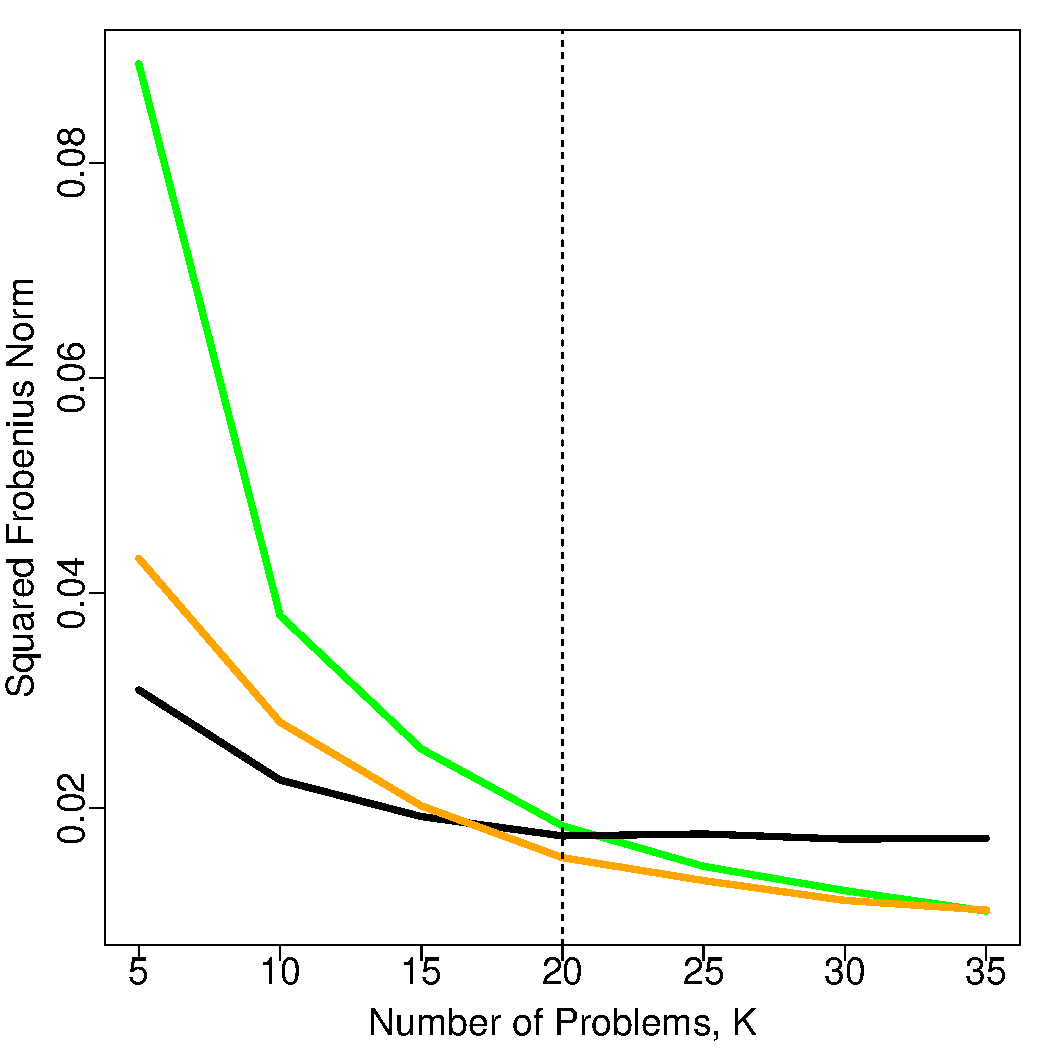
\includegraphics[width=\textwidth]{simResSigma.pdf}
                \caption{Estimation accuracy of $\bSigma$}
                \label{Sigma}
        \end{subfigure}%
        \begin{subfigure}{0.5\textwidth}
                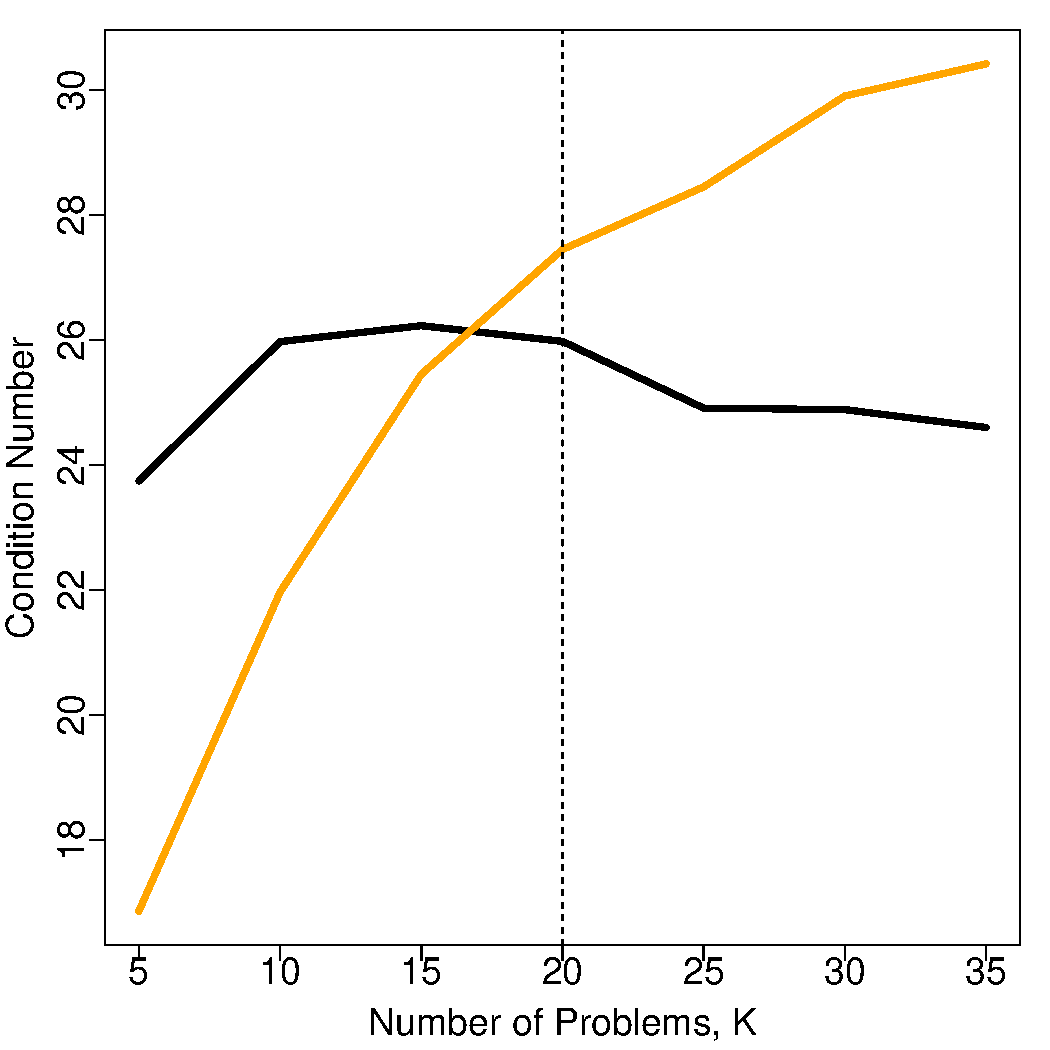
\includegraphics[width=\textwidth]{simResCond.pdf}
                \caption{Average condition numbers of the estimates}
                                \label{SigmaInv}
        \end{subfigure}
        \caption{Estimation of the information structure and the average  condition numbers of the estimates. Both are important for accurate prediction of $Y_k$. The vertical dashed lines represents the number of forecasters fixed at $N = 20$.}
        \label{SigmaEstimation}
\end{figure}


Recall  that accurate revealed aggregation stems both from a precise estimate of $\bSigma$ and a low condition number. This allows different strategies for achieving good accuracy. In fact, it turns out that the two selection procedures discussed in Section \ref{condSelection} make slightly different tradeoffs. This is illustrated in  Figure \ref{SigmaEstimation} that varies $K$ between $5$ and $35$ but keeps $N$ fixed at $20$. More specifically,  Figure \ref{Sigma} examines how $\bSigma_{cov}$,  $\bSigma_{out}$, and $\SS_Z$ capture the true $\bSigma$. 
Even though all estimators become more accurate as $K$ grows, $\bSigma_{out}$ and $\SS_Z$ improve at a higher rate than $\bSigma_{cov}$.  In fact, if $K > N$, $\SS_Z$ and $\bSigma_{out}$ perform better than $\bSigma_{cov}$. On the other hand, if $K < N$, $\bSigma_{cov}$ is more accurate than the other two. Figure \ref{SigmaInv}  presents the corresponding (average) condition numbers of these estimates. For the sake of keeping the scale manageable, $\cond(\SS_Z)$ has been omitted. Notice that $\cond(\bSigma_{out})$ increases while $\cond(\bSigma_{cov})$ generally decreases as $K$ grows larger. In fact, when $K > N$,  $\cond(\bSigma_{cov})$ is smaller than $\cond(\bSigma_{out})$. From the prediction perspective, this makes conditional-validation more forgiving towards error in the estimated $\bSigma$. Therefore, while $\bSigma_{cov}$ incorporates the actual prediction process and looks for a fine balance between a precise estimate of $\bSigma$ and a low condition number, $\bSigma_{out}$ is unaware of the details of revealed aggregation and hence simply focuses on estimating $\bSigma$ as accurately as possible. 



%Therefore an error in $\mathcal{P}_{LSE}(\cdot : \kappa_{out})$ causes a larger error in prediction.   
%  the average Frobenius norms  in estimating both $\bSigma$ and $\bSigma^{-1}$, respectively. Even though all estimators capture $\bSigma$ more accurately as $K$ grows, $\mathcal{P}_{LSE}(\cdot : \kappa_{out})$ and $\SS_Z$ improve at a higher rate than $\mathcal{P}_{LSE}(\cdot : \kappa_{cov})$.However, as was mentioned earlier, conditional validation was not designed for estimating $\bSigma$ but for predicting $Z_S$, which also requires an accurate estimate of $\bSigma^{-1}$. As can be seen in Figure  \ref{SigmaInv}, the generalized inverse of $\SS_Z$ is a poor estimate of $\bSigma^{-1}$, especially when $K$ is close to $N$. In the contrary, $\mathcal{P}_{LSE}(\cdot : \kappa_{cv})$ captures $\bSigma^{-1}$ accurately and improves as $K$ increases. 

%\begin{figure}[t!]
%\centering
%\hspace*{0em} 	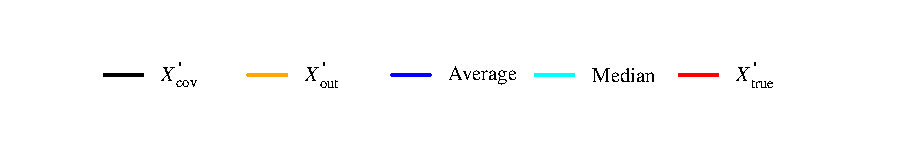
\includegraphics{legendSim2.pdf} % requires the graphicx package
%\vspace{-3.5em}
%
%                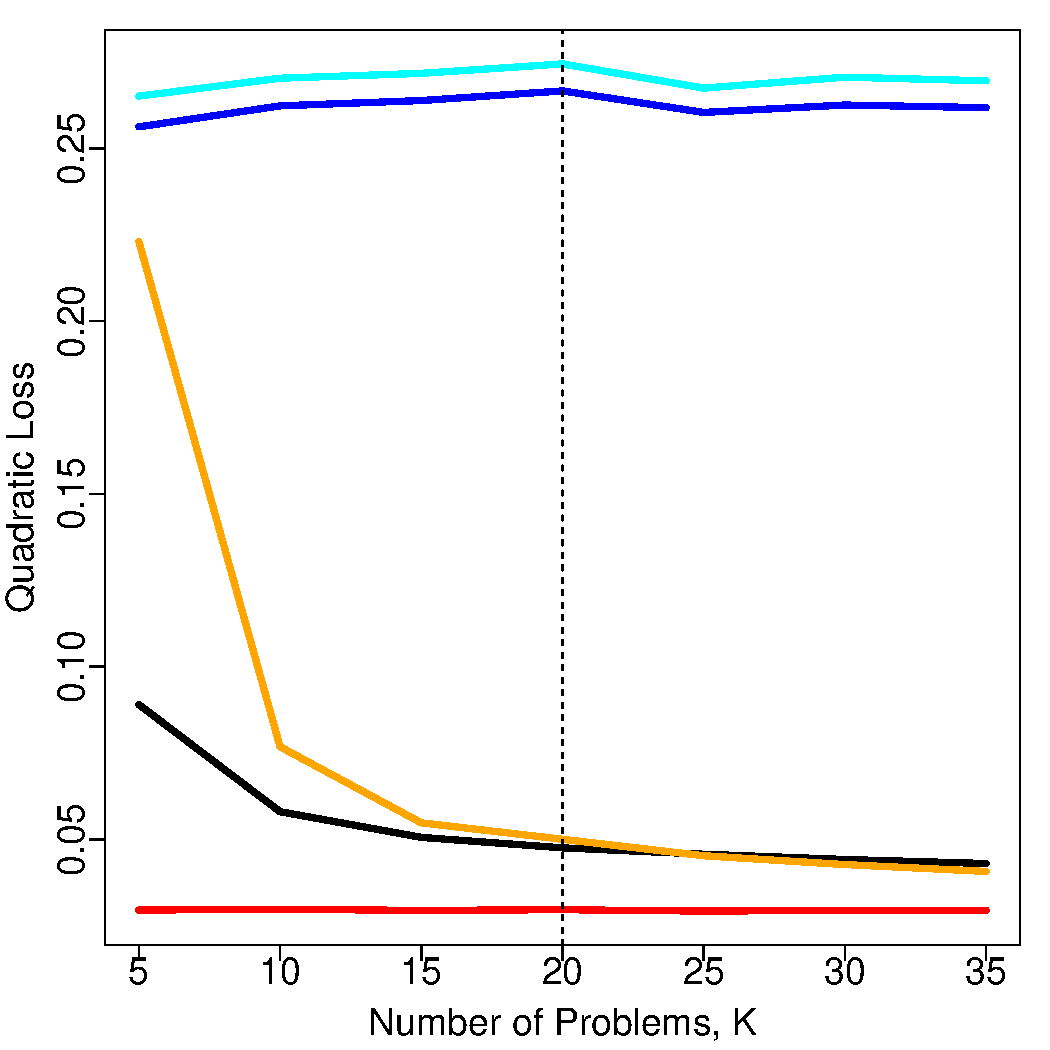
\includegraphics[width=0.5\textwidth]{simResX.pdf}
%        \caption{The accuracy to predict $Y_k$. The vertical line represents the number of forecasters, $N$, that has been fixed to $20$.}
%        \label{ZsEstimation}
%\end{figure}

\begin{figure}[t!]
\vspace{-2em}
\centering
%\vspace{-2em}
\hspace*{1em} 	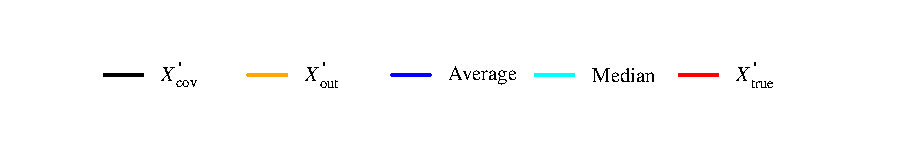
\includegraphics{legendSim2.pdf} % requires the graphicx package
\vspace{-4 em}

    	\captionsetup[subfigure]{width=0.98\textwidth }
    \begin{subfigure}{0.5\textwidth}
                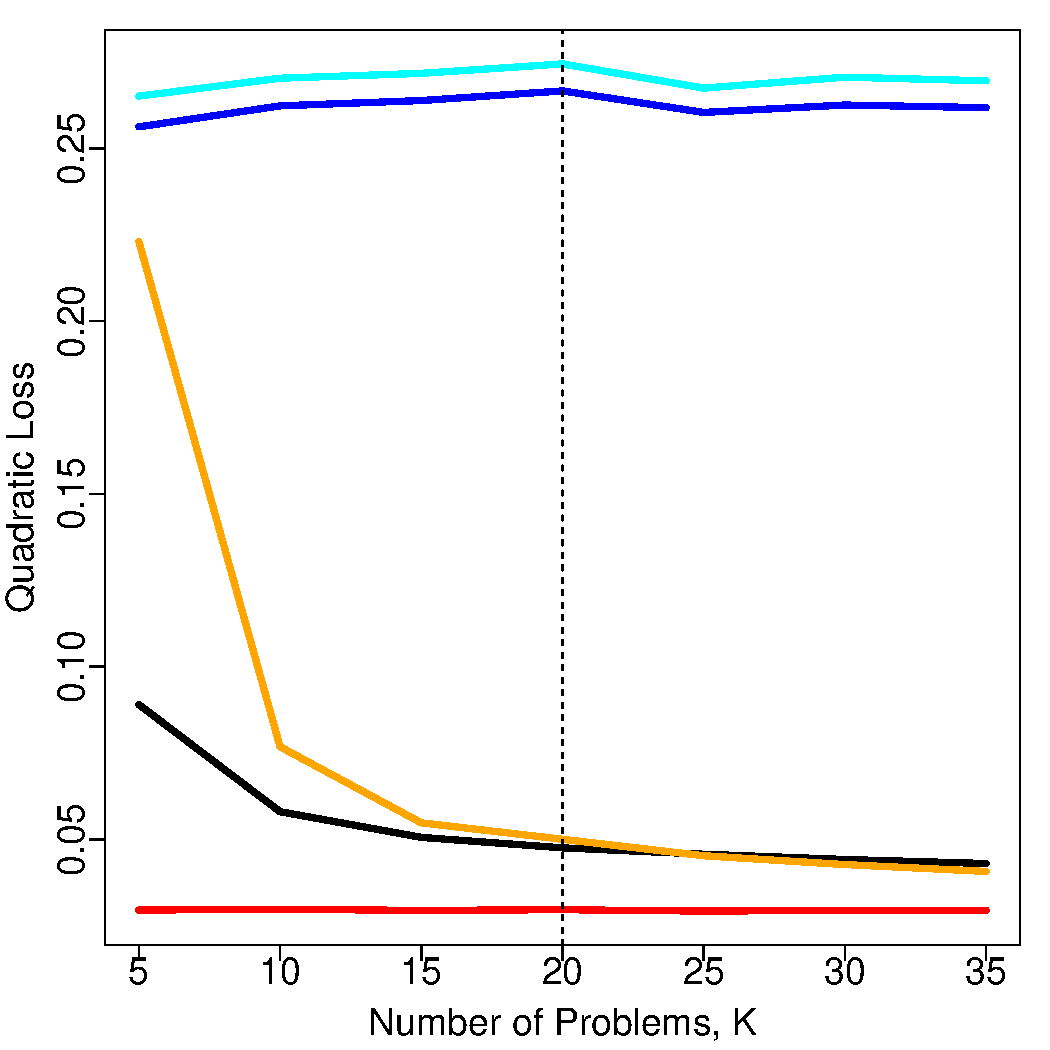
\includegraphics[width=\textwidth]{simResX.pdf}
                \subcaption{Prediction accuracy under different $K$ but fixed $N = 20$.}
                \label{Nfixed}
        \end{subfigure}%
        \begin{subfigure}{0.5\textwidth}
                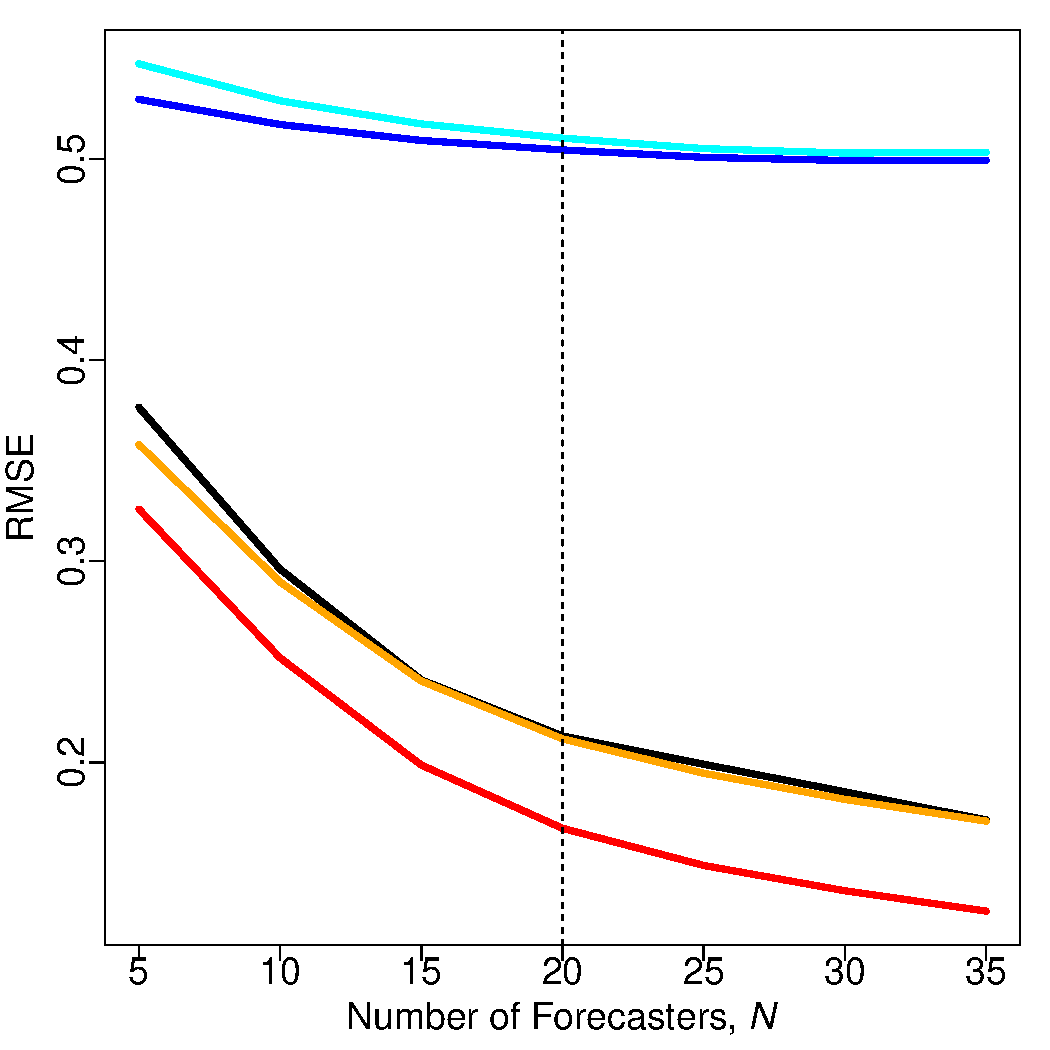
\includegraphics[width=\textwidth]{simResXN.pdf}
                \subcaption{Prediction accuracy under different $N$ but fixed $K = 20$.}
                                \label{Kfixed}
        \end{subfigure}
         \caption{The accuracy to predict $Y_k$ under different values of $N$ and $K$. The aggregator $X_{true}''$ assumes knowledge of the true information matrix and hence represents optimal accuracy.}
        \label{XEstimation}
\end{figure}

%\marginpar{Check smoothing of results}
%\marginpar{explain that first improves sigma then lower condition number}
%\marginpar{May be worth saying here that CV is good if K is large but COV is better if N is large}



These two strategies lead to slightly different predictive behavior as is illustrated in Figure \ref{XEstimation}. This plot shows the root-mean-squared-errors (RMSE) of the competing aggregators in predicting $Y_k$. Figure \ref{Nfixed} varies $K$ but fixes $N = 20$.  Figure \ref{Kfixed}, on the other hand,  varies $N$ but fixes $K = 20$. Given that $Y_k = Z_{Yk} \sim \mathcal{N}(0,1)$, the RMSE of the prior mean $\E[\sqrt{(Y_k-0)^2}] = \E[|Y_k|] = \sqrt{2/\pi} \approx 0.8$ can be considered as the upper bound in prediction error. On the other end, the aggregator $X_{true}''$ is optimal and hence provides the corresponding lower bound. The revealed aggregator $X''$ with $\SS_Z$ typically received a loss much larger than $0.8$ and is therefore not included in the figure. Overall, the average and median perform very similarly, with RMSE around $0.5$. They both show slight improvement as $N$ increases. In all cases, however, their RMSE is uniformly well above that of the revealed aggregators, suggesting that measurement-error aggregators are a poor choice when forecasts truly arise from a partial information model. The revealed aggregators $X_{cov}''$ and $X_{out}''$ perform very similarly when $K \geq 15$. They collect information and appear to improve at the optimal rate as $N$ increases. This can be seen in the way the performance gap from $X_{true}$ to  $X_{out}''$ and $X_{cov}''$ remains approximately constant as $N$ increases. The gap, however, decreases as $K$ grows larger.  When $K$ is small, say less than $15$, conditional validation is more robust and clearly yields better results. Given that conditional validation is also computationally much less demanding, only $X_{cov}''$ is considered in the following section that applies the Gaussian model to real-world forecasting data. 
  
 


%\marginpar{The averaging aggregators do not collect information, they estimate some hidden parameter instead. This is very different and strange.}


%\subsection{Simulation Study: Correctly Specified Model}
%Before the forecasts can be aggregated, it is necessary to estimate the information overlap structure. Ideally this structure would be estimated within each separate prediction problem. Unfortunately, the information structure consists of $\binom{N+1}{2}$ variables, and each problem is associated with only $N$ forecasts. Therefore, to make this estimation feasible, we assume that  the overlap structure does not change across prediction problems. Under this assumption,  all $K$ sets of forecasts can be used to estimate the overlap structure. Given that this assumption is unlikely to hold in practice, it is necessary to understand how robust the revealed aggregator is to cross-problem variation in the information structure.
%
%
%This can be examined by applying the aggregators to $K$ pairs of forecasts all drawn from the Gaussian partial information model but with different overlap structures. More specifically, the simulation first draws
%\begin{align*}
%\delta_1, \delta_2 &\sim \mathcal{U}(0,1)\\
%\rho_{12} | \delta_1, \delta_2 &\sim \mathcal{U}[\max(0,\delta_1+ \delta_2-1), \min(\delta_1, \delta_2)]
%\end{align*}
%% $\delta_1$ and $\delta_2$ uniformly at random from the interval $[0,1]$. Next the overlap parameter $\rho_{12}$ is  drawn uniformly at random from the interval $[\max(0,\delta_1+ \delta_2-1), \min(\delta_1, \delta_2)]$. 
%This ensures that the resulting overlap structure is coherent. Next two binary (column) vectors, $\boldsymbol{v}_1$ and $\boldsymbol{v}_2$, of length $L$ are constructed such that $\boldsymbol{v}_1'\boldsymbol{v}_1/L = \delta_1$, $\boldsymbol{v}_2'\boldsymbol{v}_2/L = \delta_2$, and $\boldsymbol{v}_1'\boldsymbol{v}_2/L = \rho_{12}$. These vectors represent discrete approximations of the experts' basic information. The expert, however, may know more (or less) than this about any individual problem. Therefore the overlap structure for the $k$th problem is given by $\boldsymbol{v}_{1,k}$ and $\boldsymbol{v}_{2,k}$ that are perturbed versions of $\boldsymbol{v}_1$ and $\boldsymbol{v}_2$. More specifically, for $j = 1, 2$ the vector $\boldsymbol{v}_{j,k}$ is constructed by randomly either increasing or decreasing the number of ones in $\boldsymbol{v}_j$ such that 
%%
%%by a percentage amount drawn uniformly from $[0, \Delta]$ for $j = 1,2$. Therefore 
%the largest possible difference between $\boldsymbol{v}_{j,k}'\boldsymbol{v}_{j,k}/L = \delta_{j,k}$ and $\delta_j$  is $\Delta/2$. Consequently, the maximum difference in the expert's amount of information between any two problems is $\Delta$. This provides the means for a broad yet realistic variation across problems.
%
%
%Figure \ref{Perturbation} shows the Brier scores under different levels of perturbation $\Delta$. In each case the simulation ran for a total of 10,000 iterations. During every such iteration the experts participated in $K = 30$ problems. Figure \ref{pert1} shows that the revealed aggregator $p''$ outperforms $\probit(\alpha_{opt})$ by a noticeable margin when there is no perturbation, i.e. $\Delta = 0.0$. This performance gap, however, closes as $\Delta$ approaches $0.2$. Figure \ref{pert2} shows the Brier scores when $\Delta = 0.2$. At this point the amount of information can change by $0.2$ from one problem to another, and $p''$ performs similarly to $\probit(\alpha_{opt})$. After this point $p''$ loses to the $\probit(\alpha_{opt})$ but not by too much. In fact, even when the amount of information can change by $1.0$ from one problem to another, $p''$ loses only by $0.002$. At the same time $p''$ outperforms $\probit$ by $0.005$. If the number of problems $K$ is increased from $30$ to $50$ or $100$, the value of $\Delta$ at which the performances of $p''$ and $\probit(\alpha_{opt})$ meet increases from $0.2$ to around $0.35$ and $0.45$, respectively. Therefore $p''$ is less sensitive to information variation under larger values of $K$. For the sake of brevity, these results are not presented here separately. 
% 
%This seemingly good robustness can be understood as follows: $p''$ uses the forecasts across many problems to estimate how the experts' information sets generally relate to each other. In our simulation, this relationship is defined by  $\delta_1$, $\delta_2$, and $\rho_{12}$. This information is enough for the revealed aggregator to achieve good performance on most of the problems. As $K$ increases, the revealed aggregator $p''$ can estimate the general information overlap with improved accuracy and hence present even higher robustness. 

%\marginpar{somewhere should be a discussion of when this method can be expected to work well.}

\section{Applications}
\subsection{Probability Forecasts of Binary Outcomes}
\label{binaryReal}
\subsubsection{Dataset}
%Probability forecasting is the science of giving probability estimates for future events. Typically more than one different forecast is available on the same event. Instead of trying to guess which prediction is the most accurate, the predictions should be combined into a single consensus forecast \citep{armstrong2}. The problem of aggregating probability forecasts appears in many facets of real-world applications, 
%including weather forecasting, medical diagnosis, estimation of credit default, and sports betting. 
%%including weather forecasting  \citep{murphy1977reliability}, medical diagnosis  \citep{pepe2003statistical}, estimation of credit default
%%\citep{kramer2006evaluating}, and sports betting \citep{dowie1976efficiency}.
% This section, however, focuses on predicting global events that are of particular interest to the Intelligence Advanced Research Projects Activity (IARPA). Since 2011, IARPA has posed prediction problems as a part of its ACE forecasting tournament. Among the participating teams, the Good Judgment Project (GJP) (\citealt{ungar2012good, mellers2014psychological}) has emerged as the clear winner. The GJP has recruited
%thousands of forecasters to estimate 
%probabilities of the events specified by IARPA.  The forecasters are told that their predictions
%  are assessed using the Brier score, i.e. the quadratic distance between the forecasts and the event indicator.  
%In addition to receiving \$150 for
%meeting minimum participation requirements that do not depend on
%prediction accuracy, the forecasters receive status rewards for good
%performance via leader-boards displaying Brier scores for the top 20
%forecasters. Note that, depending on the details of the reward structure, such a competition for rank may  eliminate the truth-revelation property of proper scoring rules (see, e.g., \citealt{lichtendahl2007probability}).
%The
%super-forecasters work in groups to make highly accurate predictions
%on the same events as the rest of the forecasters.

%\marginpar{this is not a case-study or through analysis of the data but an illustration of the framework}
% 
%\textit{Data.} 
%Since 2011 the Good Judgment Project (GJP) has recruited thousands of forecasters to make probability estimates on different geopolitical events. 
During the second year of the Good Judgment Project (GJP) the forecasters made probability estimates for $78$ events, each with two possible outcomes. One of these events was illustrated in Figure \ref{Example_prob}. %Since 2011 t%Before the forecasts can be aggregated, however, several practical matters must be discussed. First, 
Each prediction problem had a timeframe, defined as the number of days between the first day of forecasting and the anticipated resolution day. 
% during which the forecasters make and update their predictions. 
%To illustrate, two of
%the questions were: The predictions made for these two events are shown in Figure \ref{Examples}.
% The prediction problem closes and no more forecasts are allowed once the corresponding event resolves. 
These timeframes varied largely among problems, ranging from 12 days to 519 days with a mean of 185.4 days.
% 
%  For instance, the events in Figures \ref{Example1} and \ref{Example2} have timeframes of 154 and 52 days, respectively. 
During each timeframe the forecasters were allowed to update their predictions as frequently as they liked.  The forecasters knew that their estimates would be assessed for accuracy using the quadratic loss. 
%Brier scores, i.e., the squared distance between the probability forecast and the event indicator that equals $1.0$ or $0.0$ depending on whether the event happened or not, respectively. 
This is a revealing loss function that incentivized the forecasters to report their true beliefs instead of attempting to game the system. In addition to receiving \$150 for meeting minimum participation requirements that did not depend on prediction accuracy, the forecasters received status rewards for their performance via leader-boards displaying the losses for the best $20$ forecasters. Depending on the details of the reward structure, such a competition for rank may eliminate the truth-revelation property of revealing loss functions (see, e.g., \citealt{lichtendahl2007probability}).


%This data raises several issues: First, recall that the partial information framework is designed for noise-reduction. Therefore the forecasts are assumed to be conditionally unbiased, i.e., \textit{calibrated}, as this condition is more often called in the probability forecasting literature. Unfortunately, human experts are generally known to lack calibration. Simple calibration measures suggest that this is also the case with the GJP forecasters. Even though the level of calibration can be somewhat improved via pre-processing mechanisms, such as Platt scaling \citep{platt1999probabilistic} or Isotonic regression \citep{zadrozny2001obtaining}, these techniques require a training set with known outcomes and are hence outside the scope of this paper. 

%The results, however, suggest that the revealed aggregator remains robust and is able out-perform competing aggregators even when the forecasts are not extremely well-calibrated. 

This data collection raises several issues: First, given that the current paper does not focus on modeling dynamic data, only forecasts made within some common time interval should be considered.  The final outcome is typically the most uncertain in the beginning but becomes fully certain by the resolution date. 
%Therefore the goal is to choose some mid-interval during which predicting the correct outcome is neither trivial nor extremely difficult because in both of these cases the competing aggregators are unlikely to present meaningful differences.
 Second, not all forecasters made predictions for all the events. Furthermore, the forecasters generally updated their forecasts infrequently, resulting into a very sparse dataset. Such high sparsity can cause problems in  computing the initial unconstrained estimator $\SS$. 
%Under a large number of missing observations, one option is to simply use all the complete pairs of observations.  This requires any two forecasters to make predictions on at least two common problems. 
Evaluating different techniques to handle missing values, however, is well outside the scope of this paper. Therefore, to somewhat alleviate the effect of missing values, only the hundred most active forecasters are considered. This makes sufficient overlap highly likely but, unfortunately, still not guaranteed. 


% Requires the booktabs if the memoir class is not being used
\begin{table}[t!]
   \centering
   \caption{Summary of the three time intervals analyzed. Each scenario considers the forecasters' most recent forecasts within the given time interval. The value in the parentheses represent the number of events occurred. The final column shows the percent of missing forecasts. }
   \begin{tabular}{l ccc } % Column formatting, @{} suppresses leading/trailing space
   \hline\hline
      Scenario      & Time Interval & \# of Events & Missing (\%)  \\\hline
      High Uncertainty (HU)        & $90-120$     & $49$ $(10)$ & $51$\\ 
      Medium Uncertainty (MU)       & $60-90$  &  $56$ $(14)$  & $46$ \\
      Low Uncertainty (LU) &  $30-60$ & $60$ $(13)$ & $42$\\ \hline
   \end{tabular}
   \label{scenarios}
\end{table}

All these considerations lead to a parallel analysis of three scenarios: High Uncertainty (HU), Medium Uncertainty (MU), and Low Uncertainty (LU). Important differences are summarized in Table \ref{scenarios}. Each scenario considers the forecasters' most recent prediction within a different time interval.  For instance, LU only includes each forecaster's most recent forecast during $30-60$ days before the anticipated resolution day. The resulting dataset has $60$ events of which $13$ occurred. In the corresponding $60 \times 100$ table of forecasts, around 42 \% of the values are missing. The other two scenarios are defined similarly. 

%Notice that the amount of data increases monotonically from HU to LU. Therefore the relative advantage of revealed aggregation can be expected to be smallest under HU and largest under LU. 


% \begin{enumerate}[a)]
%\item \textit{Lower Uncertainty (LU):} Consider each forecaster's most recent forecast during $30-60$ days before the anticipated resolution day. The resulting dataset has $60$ events of which $13$ occurred. There are $841$ forecasters attending, on average, $11.3$ problems, with a range of $1$ to $55$ problems. The top $100$ most active forecasters attended, on average, $34.9$ problems, with a range of $25$ to $55$ problems. In the resulting $60 \times 100$ data table, around 42\% of the values are missing. 
% 
%\item \textit{Higher Uncertainty (HU):} Consider each forecaster's most recent forecast during  $90-120$ days before the anticipated resolution day. The resulting dataset has $49$ events of which $10$ occurred. There are $732$ forecasters attending, on average, $7.7$ problems, with a range of $1$ to $46$ problems.  The top $100$ most active forecasters attended, on average, $24.0$ problems, with a range of $14$ to $46$ problems. In the resulting $49 \times 100$ data table, around 51\% of the values are missing. 
% \end{enumerate}
 
%Another study looking at the $60-90$ days before the anticipated resolution day was also conducted. The results, however, were qualitatively very similar to the results presented in the following sections. Therefore, to minimize redundancy, this middle scenario was omitted from the paper.  




%``Will Zimbabwe commence a presidential election before 1 January 2013?". This question became available to the forecasters on 21 February 2012. Predictions were allowed until the event resolved; that is, until 1 January 2013 or the day Zimbabwe commences a presidential election, depending which one comes first. Given that Zimbabwe did not commence  the election before 1 January 2013, the final day of forecasts was 30 December 2012, giving a timeframe of  313 days of active forecasting. 

%The focus of this paper, however, is not on such dynamic data. Instead, the goal is to model 
%Overall, the number of days left before the resolution date is a strong indicator of the level of uncertainty in the event. This uncertainty then vanishes as the resolution data approaches. To standardize uncertainty to a non-trivial level without discarding too much data,  

% IFP is 1094

%\marginpar{the distribution of lens is very right skewed with most problems having a len of about median is 71}

%\marginpar{These  are binary problems.}
%
% As was mentioned in Section \ref{context}, the partial information framework is designed for noise reduction. Therefore the forecasts are assumed to be conditionally unbiased. A conditionally unbiased forecaster making probability estimates is typically called \textit{calibrated} in the forecasting literature. Given that forecasters are generally not well-calibrated, data transformations for improving calibration have been developed. Probably the most well-known such technique is Platt scaling that transform the forecasts with a sigmoidal function \citep{platt1999probabilistic}. More specifically, consider $K$ events $A_1, \dots, A_K$ and forecaster $i$'s corresponding probability estimates $p_{1i}, \dots, p_{Ki}$. Let $K_+$ and $K_-$ be the number of events that happened and did not happen, respectively. Platt scaling then finds
% \begin{align*}
%\argmin_{A_i,B_i} \left\{ - \sum_{k=1}^K Y_k \log(S(p_{ki})) + (1-Y_k)\log(1-S(p_{ki})) \right\},
% \end{align*}
% where $S(p) = 1/(1+\exp(A_ip + B_i))$ and $Y_k$ is equal to $(K_++1)/(K_+ + 2)$ or $1/(K_- + 2)$ depending on whether $A_k$ happened or not, respectively. This, of course, requires  the outcomes of the events. Therefore the calibration parameters $A_i$ and $B_i$ are learned based on the first-year problems. These values are then used to calibrated the second-year forecasts. To evaluate sensitivity to changes in calibration, aggregation is applied to the second-year forecast both before and after calibration. 
% 
%Not all the GJP forecasters made predictions for all the events, making the data fairly sparse.
%% Given that learning the calibration parameters based on a few events and probability estimates can lead to drastic overfitting, only forecasters who participated in at least half of the first-year problems were considered.  
%% 
%The Gaussian model can be applied as long as an unconstrained estimator $\SS_Z$ is available. Under a large number of missing observations, one option is to simply use all the complete pairs of observations to estimate the corresponding covariance.  This requires any two forecasters to make predictions on at least two common problems. However, given that evaluating different techniques to handle missing values is well outside the scope of this paper,  sufficient overlap is guaranteed by
%%This can be challenging from the partial information perspective because the information overlap can be estimated between two forecasters only if they both made predictions on a number of common problems. 
%considering only the hundred most active forecasters. The number of problems participated by these forecasters ranged from $30$ to $47$, with an average of $38.55$ problems. Recall that the forecasters were allowed to update their forecasts until the event resolved. To choose one prediction per forecaster, this paper analyzes two different setups: the \textit{higher uncertainty} (HU) setup considers only the forecaster's first prediction while the \textit{lower uncertainty} (LU) setup considers only the forecaster's last prediction. 
%%\begin{enumerate}[a)]
%%\item\textit{Higher Uncertainty:}  consider only the forecaster's first prediction, and
%%\item\textit{Lower Uncertainty:}  consider only the forecaster's last prediction.
%%\end{enumerate} 
%The forecasts under HU are generally less accurate than the forecasts under LU because they are made earlier when the event presents relatively higher level of uncertainty. 
% 
 
 
 







%This subsection focuses on the super-forecasters in the second year of the tournament. Given that these forecasters were
%elected to the group of super-forecasters based on the first year, 
%%Our evaluation, however, only uses forecasts that were made
%%during the second year. 
% their forecasts are
%likely, but not guaranteed, to be relatively good. The group involves 44 super-forecasters collectively making predictions about  123 events, of which 23 occurred. 
% For instance, some of
%the questions were: ``Will France withdraw at least 500 troops from Mali before 10 April 2013?", and ``Will a banking union be approved in the EU council before 1 March 2013?". 
%%(see the Appendix in \citealt{satopaa} for more descriptions).  
%%The forecasters were allowed to update their predictions as long as the
%%questions remained active. 
%%Some questions were active longer than the
%%others. More specifically, the number of active days ranged from 3 to 284 days,
%%with a mean of 96 days. The super-forecasters tended to update their predictions quite frequently. 
%%The number of active days ranged from 3 to 284 days, with a mean of 96 days. 
%%In this paper, however, only the most recent prediction made within the first three days of each problem is considered.  
%%In the resulting
%%dataset,
%Not every super-forecaster made predictions about every event. In fact, 

\subsubsection{Model Specification and Aggregation}
%\vspace{2em}
%\noindent
%\textit{Model.} 
The fact that  $Y_k \in \{0,1\}$ is binary and lies on the boundary of the support of the forecasts $X_{jk} \in [0,1]$ makes the model instance slightly more involved. This instance resembles in many ways the latent variable version of a standard probit model. 
\begin{quote}
\textbf{Model Instance.} Represent the $k$th event with $Y_k \in \{0,1\}$ for $k = 1, \dots, K$. These outcomes link to the Gaussian information pool via the following function:
\begin{align*}
Y_k &= g(Z_{Yk}) = \begin{cases}
1 & \text{ if } Z_{Yk} > t_k\\
0 & \text{ otherwise},\\
\end{cases}
\end{align*}
where $t_k \in \R$ is some threshold value. Therefore the link function $g(\cdot)$ is simply the indicator function $\one_{A_k}$ of the event $A_k = \{Z_{Yk} > t_k\}$. The prior probability of the $k$th event is $\P(Y_k = 1) = \Phi(-t_k)$, where $\Phi(\cdot)$ is the CDF of a standard Gaussian distribution. Given that the thresholds are allowed to vary among the events, each event has its own prior. 
%Overall, the events are quite different. Therefore it is important to allowing the threshold $t_k$ to change across problems. 
The corresponding probability forecasts $X_{jk} \in [0,1]$ are
\begin{align*}
X_{jk} &= \E[Y_k | Z_{jk}] = \Phi\left( \frac{Z_{jk} - t_k}{\sqrt{1-\delta_j}}\right).
\end{align*}
In a similar manner, 
% if $\Z_k = (Z_{B_1, k}, \dots, Z_{B_N, k})'$ collects the forecasters' information variables, then 
 the revealed aggregator $X_k'' \in [0,1]$ for event $k$ is
\begin{align}
X_{k}'' &= \E[Y_k | \Z_k] = \Phi\left( \frac{\diag(\bSigma)'\bSigma^{-1}\Z_k - t_k}{\sqrt{1-\diag(\bSigma)'\bSigma^{-1}\diag(\bSigma)}}\right). \label{RevAgg}
\end{align}
%\vspace{2em}
%\noindent
%\textit{Estimation.} 
\end{quote}

%\marginpar{this largely resembles the probit model and hidden variables. Should mention this. Makes it seem clearer.}

%\marginpar{We need to explain somewhere how we handle sparsity: gaussian dropping some terms is still gausisan with the given covariance sub matrix}

%\marginpar{it may be worth discussing the difference between the initial estimate of tk and the final precision weighted one.}

All the parameters of this model can be estimated from the data. The first step is to specify a version of the  unconstrained estimate $\SS$. If the $t_k$'s do not change much, a reasonable and simple estimate is obtained  by transforming the sample covariance matrix  $\SS_P$ of the probit scores $P_{jk} := \Phi^{-1}(X_{jk})$. More specifically,  if $\D := \Diag( \dd ) \Diag(\one + \dd)^{-1}$, where $\dd = \diag(\SS_P)$, then an unconstrained estimator of $\bSigma$ is given by $\SS = (\I_N-\D)^{1/2} \SS_P (\I_N-\D)^{1/2}$. Recall that the GJP data holds many missing values. This is handled by estimating each pairwise covariance in $\SS_P$ separately based on all the events for which both forecasters made predictions. 
%If the predictions are missing at random, the resulting $\SS_P$ is an unbiased estimator of $\Cov(\PP)$. 
Next, compute $\bSigma_{cov}$, where $\kappa_{cov}$ is chosen over a grid of $100$ candidate values between $10$ and $1,000$. 
%Once the final estimate of $\bSigma$ has been found,
The threshold $t_k$ can be estimated by letting $\PP_k = (P_{1k}, \dots, P_{Nk})'$, observing that $-\Diag(\one-\diag(\bSigma))^{1/2}\PP_{k} \sim \mathcal{N}_N(t_k \one_N, \bSigma)$,
%With this estimate of $\bSigma$, the thresholds $t_k$ can be estimated.
% It is possible  $t_k$ is set by the prior $\P(A_k)$; that is, if $\P(A_k) = q_k \in [0,1]$, then $t_k = \Phi^{-1}(1-q_k)$. Alternatively, the value of $t_k$ can be estimated from the forecasts by 
% 
% observing that $P_{jk} := -\Phi^{-1}(X_{jk})\sqrt{1-\delta_j} \sim \mathcal{N}(t_k, \delta_j)$. 
and finally computing the precision-weighted average: 
\begin{align*}
%\hat{t}_k &= -\frac{\sum_{j=1}^N \sqrt{1-\hat{\delta}_j}P_{jk}/\hat{\delta}_j}{\sum_{j=1}^N 1/\hat{\delta}_j},
\hat{t}_k &= -\frac{\PP_{k}' \Diag(\one-\diag(\bSigma_{cov}))^{1/2} \bSigma_{cov}^{-1} \one}{\one' \bSigma_{cov}^{-1} \one}.
\end{align*}
 If $\PP_k$ has missing values, the corresponding rows and columns of $\bSigma_{cov}$ are dropped. Intuitively, this estimator gives more weight to the forecasters with very little information. Plug these estimates in (\ref{RevAgg}) to get the revealed aggregator  $X_{cov}''$. 


%\vspace{2em}
%\noindent
%\textit{Analysis.} 
This aggregator is benchmarked against the state-of-the-art measurement-error aggregators, namely the average probability, median probability, average probit-score, and average log-odds. To avoid infinite log-odds
and probit scores, extreme forecasts $X_{jk} = 0$ and $1$ were
censored to $X_{jk} = 0.001$ and $0.999$, respectively. The results remain insensitive to the exact choice of censoring as long as this is done in a reasonable manner to keep the extreme probabilities from becoming highly influential in the logit- or probit-space. Similarly to before, the accuracy of the aggregates is measured with the RMSE.
% $X_k$ is measured with the mean Brier score (BS) defined as quadratic loss between the aggregate and the event indicator:
%%Consider $K$
%%events and collect all $N_k$ probability forecasts for event $A_k$ into a vector $\boldsymbol{p}_k \in [0,1]^{N_k}$. Then, BS for aggregator $\text{Agg}:[0,1]^{N_k} \to [0,1]$ is 
% \begin{align*}
%\text{BS} &= \frac{1}{K} \sum_{k=1}^K \left(X_k- \one_{A_k}\right)^2.
% \end{align*}
%This score takes values within the unit interval with lower values suggesting better accuracy.
 Instead of considering all the forecasts at once, the aggregators are evaluated under different $N$ via repeated subsampling of the $100$ most active forecasters; that is, choose $N$ forecasters uniformly at random, aggregate their forecasts, and compute the RMSE. This is repeated 1,000 times with $N = 5, 10, \dots, 50$ forecasters. In the rare occasion where no pairwise overlap is available between one or more pairs of the selected forecasters, the subsampling is repeated until all pairs have at least one problem in common. 
%The simulation study is performed separately for the HU and LU setups. 



\begin{figure}[t!]
\vspace{-2em}
\centering
\hspace*{1em} 	
\includegraphics[width=\textwidth]{legendReal.pdf} % requires the graphicx package
\vspace{-4em}

        \centering
        \begin{subfigure}{0.32\textwidth}
                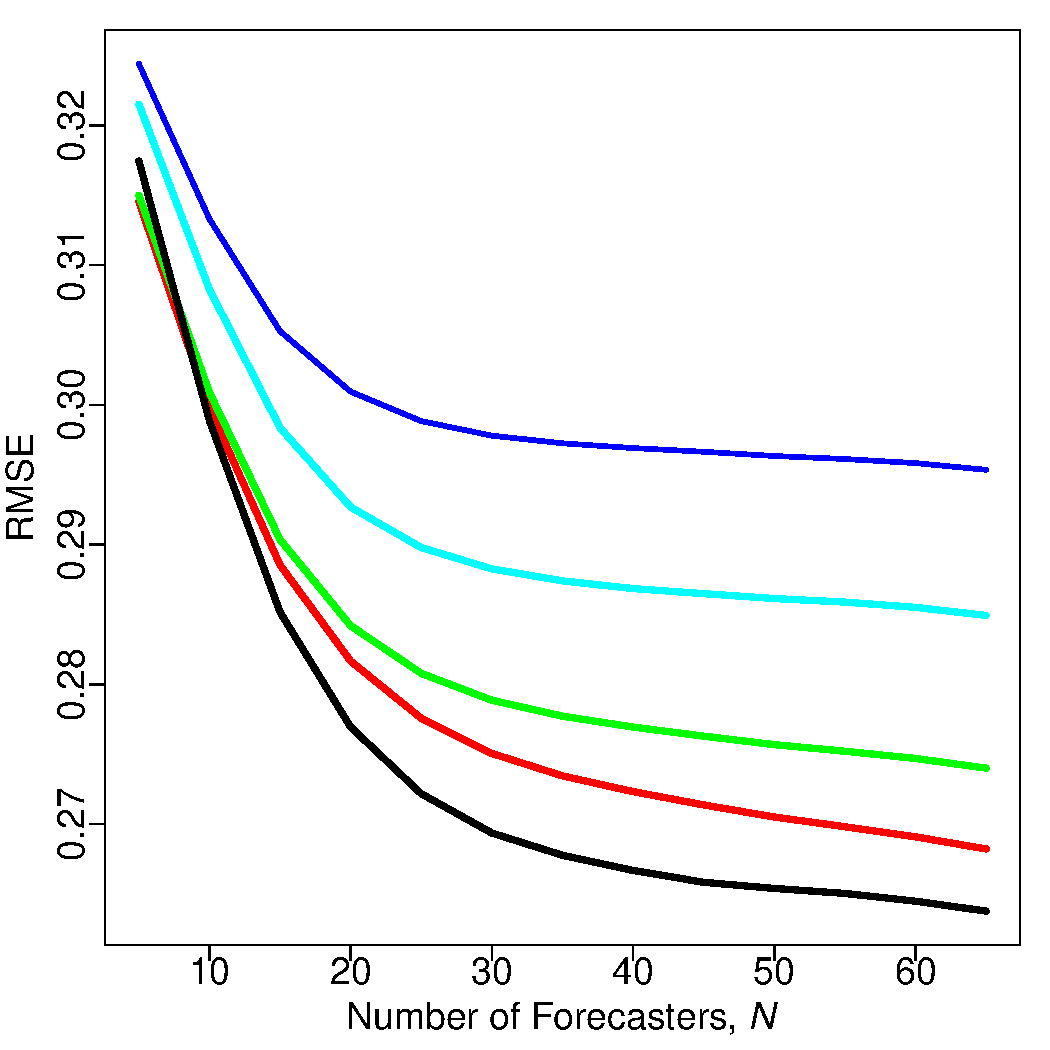
\includegraphics[width=\textwidth]{realHU}
                \caption{High Uncertainty (HU)}
                                \label{highUnc}
        \end{subfigure}
        \begin{subfigure}{0.32\textwidth}
                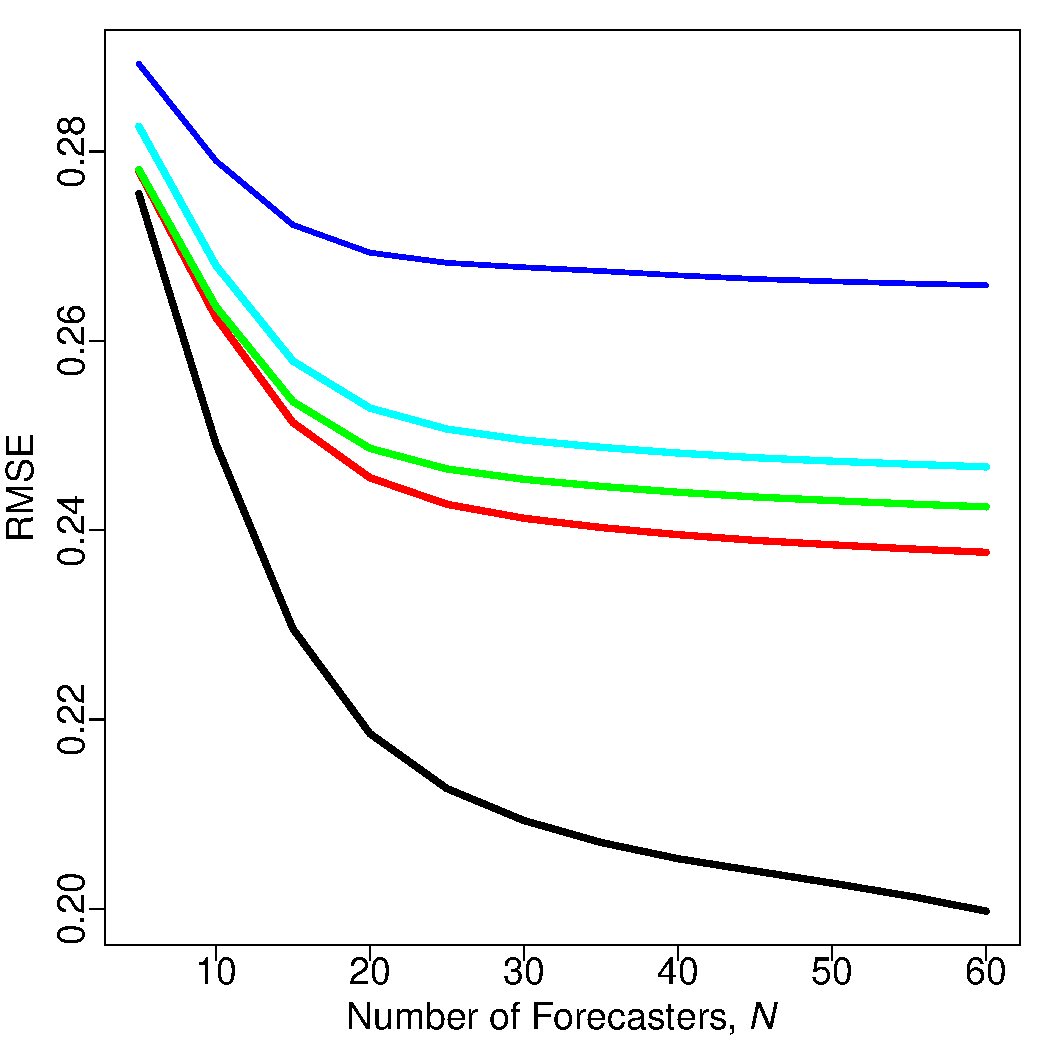
\includegraphics[width=\textwidth]{realMU}
                \caption{Medium Uncertainty (MU)}
                                \label{medUnc}
        \end{subfigure}
        \begin{subfigure}{0.32\textwidth}
                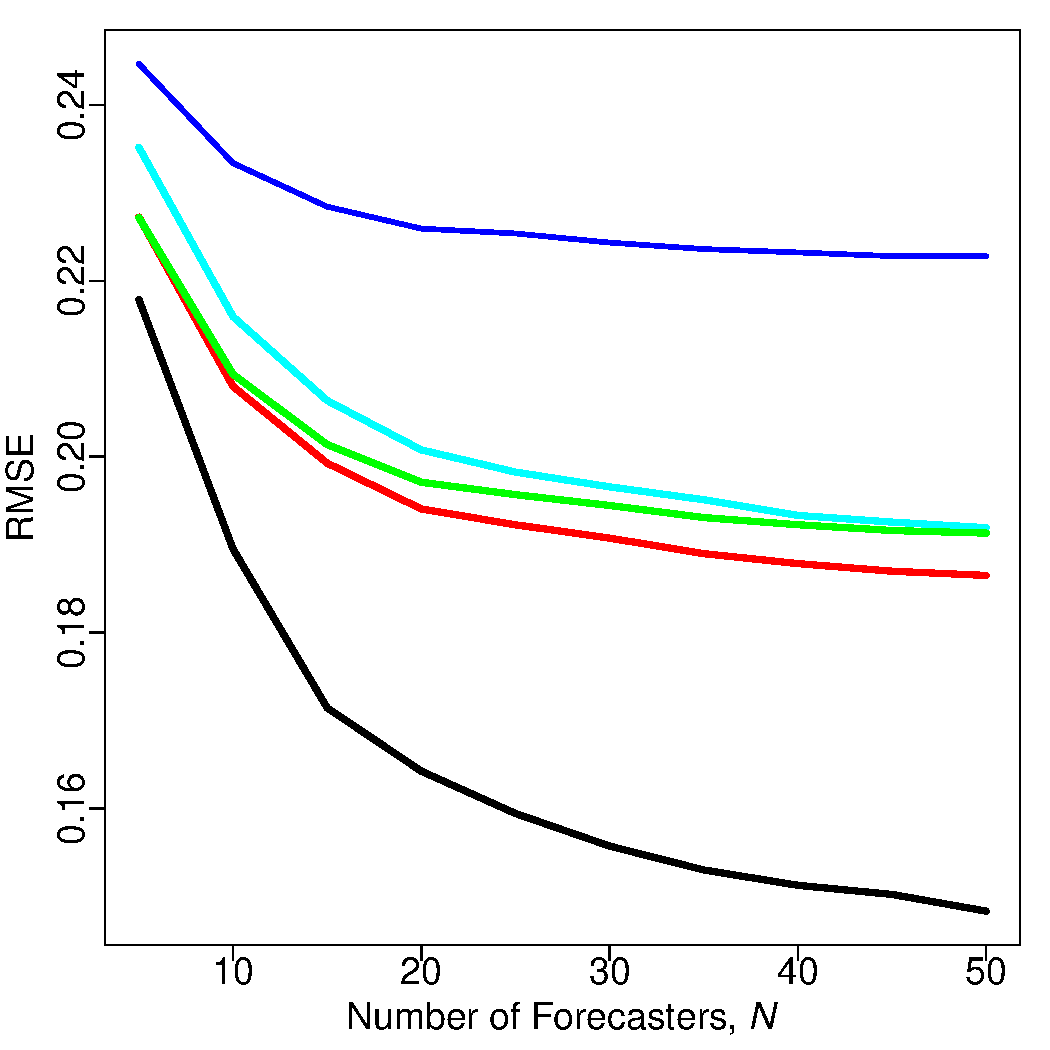
\includegraphics[width=\textwidth]{realLU}
                \caption{Low Uncertainty (LU)}
                                \label{lowUnc}
        \end{subfigure}             
        
        \caption{Average prediction accuracy over the 1,000 sub-samplings of the forecasters. See Table \ref{scenarios} for descriptions of the different scenarios.}
        \label{simReal}
\end{figure}


Figure \ref{simReal} shows the average RMSE's under the three scenarios described in Table \ref{scenarios}. Notice that the scores become uniformly worse from HU to LU. This reflects the decreasing level of uncertainty. 
%All scenarios, however, tell a similar story about the relative accuracies of the competing aggregators. First,
In all the figures the measurement-error aggregators rank in the typical order (from worst to best): average probability, median probability, average probit, and average log-odds. Despite the level of uncertainty, the revealed aggregator $X_{cov}''$ outperforms the averaging aggregators as long as $K \geq 10$. 
%This provides evidence in favor of information diversity being the more important source of forecast heterogeneity. 
The relative advantage, however, increases from HU to LU. This trend can be explained by several reasons: First, as can be seen in Table \ref{scenarios}, the amount of data increases from HU to LU. This yields a better estimate of $\bSigma$ and hence more accurate revealed aggregation. Second, under HU the events are still inherently very uncertain. Consequently, the forecasters are unlikely to hold much useful information as a group. Under such low information diversity, measurement-error aggregators generally perform relatively well (\citealt{satopaamodeling}).  In the contrary, under MU  the events have lost a part of their inherent uncertainty, allowing some forecasters to possess useful private information. These individuals are then prioritized by $X_{cov}''$ while the averaging-aggregators continue treating all forecasts equally. Third, the forecasters can be expected to show better calibration under MU and LU than under HU. Therefore the model assumptions are more likely to hold under MU and LU. 
%  $X_{cov}''$ is able to collect information more efficiently than the measurement error aggregators. Consequently, its performance advantage grows as $N$ increases. 
%Overall, the extent to which $X_{cov}''$ outperforms the measurement-error aggregators 
% model of forecast heterogeneity than measurement error. 


% practical evidence in favor of information diversity as the dominating source of heterogeneity. 

%Consequently,  $\mathcal{P}_{LSE}(\cdot : \kappa_{out})$  achieves the best score for  $N \geq 15$, with the performance advantage growing in $N$. Fourth, even though $\mathcal{P}_{LSE}(\cdot : \kappa_{out})$ outperforms $\mathcal{P}_{LSE}(\cdot : \kappa_{in})$ for small $N$, this advantage diminishes as $N$ grows. In fact, for $N \geq 30$,  $\mathcal{P}_{LSE}(\cdot : \kappa_{in})$ outperforms $\mathcal{P}_{LSE}(\cdot : \kappa_{out})$. This suggests the use of the computationally less demanding $\mathcal{P}_{LSE}(\cdot : \kappa_{out})$ under large $N$. 




 
%
%For a more detailed performance analysis, it decomposes into three additive components: reliability (REL),
%resolution (RES), and uncertainty (UNC). This assumes
%that the aggregate forecast $g(\boldsymbol{p}_k)$ for all $k$ can only take discrete values $f_j \in
%[0,1]$ with $j = 1, \dots, J$. Let $n_j$ be the number of times $f_j$
%occurs, and denote the empirical frequency of the corresponding events
%with $o_j$.  Let $\bar{o}$ be the overall empirical frequency of
%occurrence, i.e., $\bar{o} = \frac{1}{K} \sum_{k=1}^K  \one_{A_k}$. Then,
% \begin{align*}
%\text{BS} &= \text{REL} - \text{RES} + \text{UNC}\\
%&= \frac{1}{K} \sum_{j=1}^J n_j (f_j - o_j)^2 - \frac{1}{K} \sum_{j=1}^J n_j (o_j - \bar{o})^2 + \bar{o}(1-\bar{o}).
% \end{align*}
% Confident aggregators exhibit high RES.
%%High RES indicates a confident aggregator.
%%and hence very different from to the naive forecast $\bar{o}$. 
%The corresponding forecasts are likely to be very close to $0$ and $1$, which is more useful to the decision-maker than the naive forecast $\bar{o}$ as long as the forecasts are also accurate, i.e., calibrated. In the decomposition, good calibration presents itself as low REL. Therefore both improved calibration and higher confidence yield a lower BS. Any such improvements should be interpreted relative to UNC that equals the BS for $\bar{o}$, i.e., the best aggregate that does not use the forecasters' predictions.
%



%\marginpar{Explain why this dataset is actually not very appropriate for our model: assuming a constant information structure is not a very plausible. The problems are quite different. }



 
 


%\marginpar{Make two separate sections: a) random sampling of experts and aggregation, b) explain that "where would this diversity come from: well, we have some prior knowledge of information overlap such as groups, supers etc. Let's look at a instance where this is particularly clear.}

%\marginpar{discuss estimating Estimating $t$ or $\P(A)$; the problem is that this parameter only exists under binary estimation problems.}
%
%\marginpar{Discuss poor calibration}





\subsubsection{Information Diversity}
%The averaging-like aggregators can be expected to work well when the forecasters have very similar information sets \citep{satopaamodeling}. 

This subsection examines how closely the estimated $\bSigma$ reflects prior knowledge about the forecasters' information structure. 
%The extent to which the revealed aggregator outperforms the averaging-aggregators, however, suggests that the GJP forecasters use very different information sets. This is not surprising because the individuals generally have different  interests and background knowledge.
%More specifically, some sources of information diversity were controlled.
 In particular, the GJP assigned the forecasters to make predictions either in isolation or in teams. Furthermore, after the first year of the tournament, the top 1\% forecasters were elected to the elite group of ``super-forecasters''. These super-forecasters then worked in exclusive teams to make highly accurate predictions on the same events as the rest of the forecasters. Many of these characteristics directly suggest a level of information overlap. For instance, super-forecasters can be expected to have the highest $\delta_j$'s and forecasters in the same team should have a relatively high $\rho_{ij}$. 

%the extent to which our prior knowledge on information overlap coincides with the estimated $\bSigma$. 


\begin{figure}[t!]
        \centering
        \begin{subfigure}[b]{0.495\textwidth}
                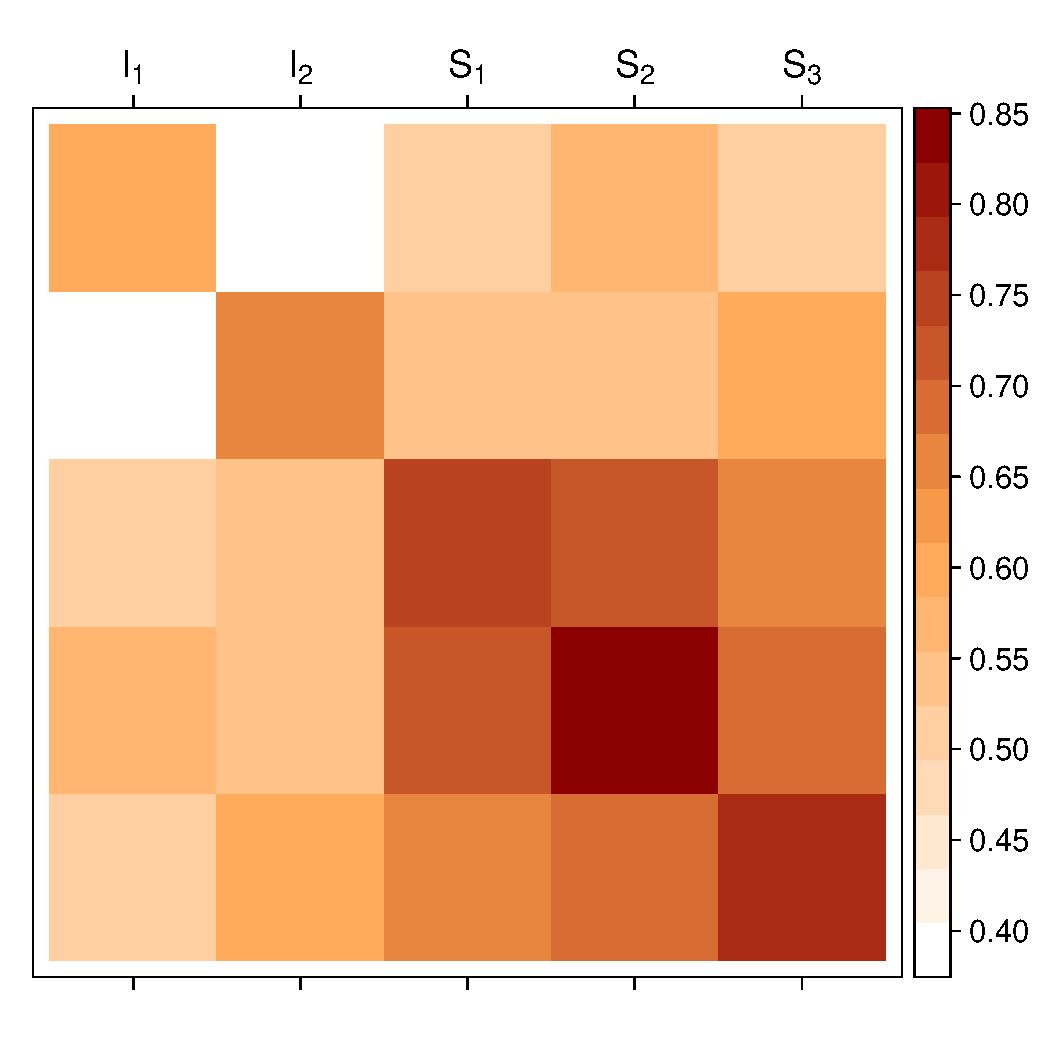
\includegraphics[width=\textwidth]{leftInfoPlot.pdf}
                \caption{The five most active forecasters}
                \label{top5}
        \end{subfigure}%
        %\begin{subfigure}{0.455\textwidth}
        \begin{subfigure}[b]{0.495\textwidth}
        \hspace*{-11em} 	
\includegraphics{legendSigmaAll.pdf} % requires the graphicx package
\vspace{-4.5em}

                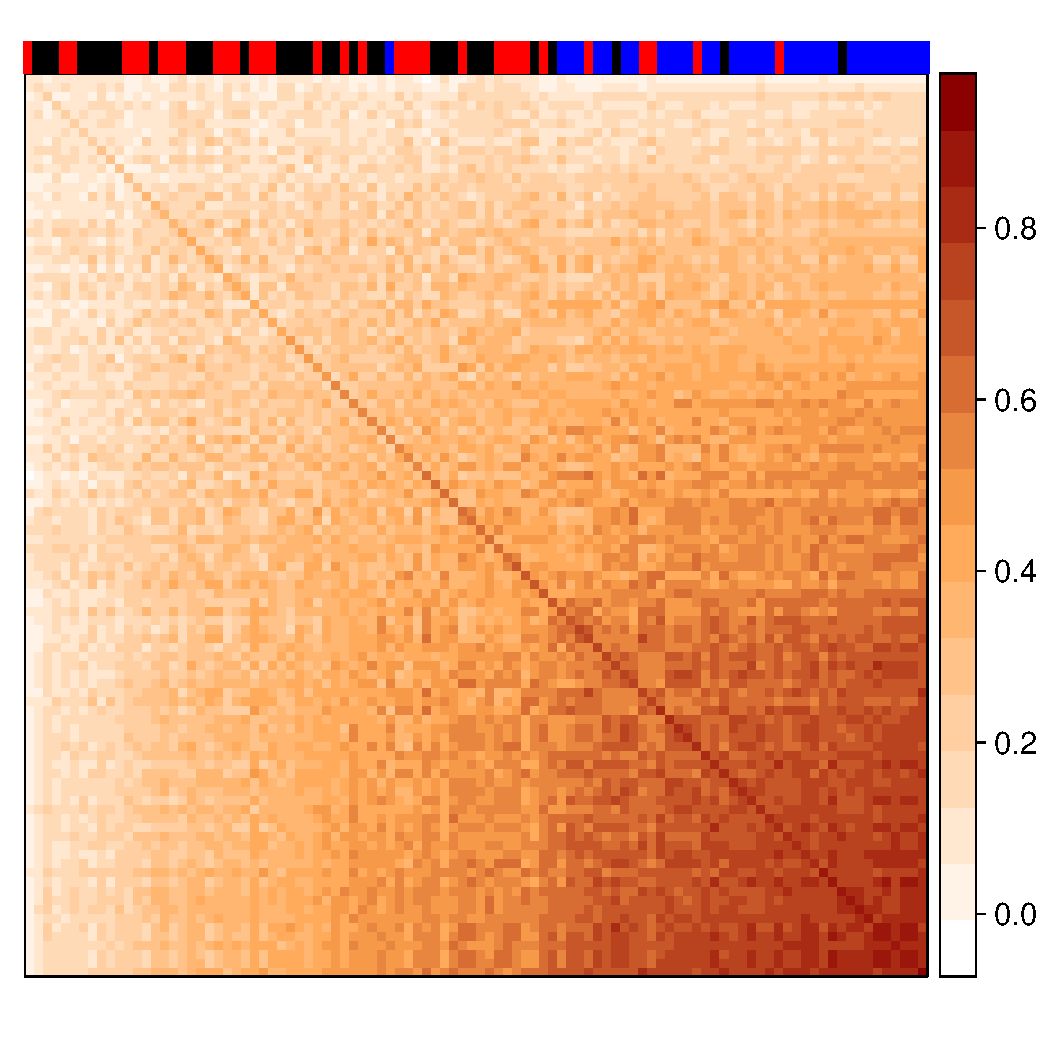
\includegraphics[width=0.95\textwidth]{rightInfoPlot.pdf}
%	\vspace{0.8em}
            \caption{All 100 forecasters}
                                \label{top100}
        \end{subfigure}

       
        \caption{The estimated information structure $\bSigma$ under the LU scenario. Each forecaster worked either in isolation, in a non-super-forecaster team, or in a super-forecaster team. The super-forecasters generally have more information than the forecasters working in isolation.}
        \label{SynthPlot}
\end{figure}

%% 4470 and 1119 and  2763, 5265, and 4916

For the sake of brevity, only the LU scenario is analyzed as this is where $X_{cov}''$ presented the highest relative improvement. 
The associated 100 forecasters involve 36 individuals predicting in isolation, 33 forecasting team-members (across 24 teams), and 31 super-forecasters (across 5 teams).  Figure \ref{top5} displays $\bSigma_{cov}$ for the five most active forecasters, involving two forecasters working in isolation (Iso. A and B) and three super-forecasters (Sup. A, B, and C). Only the super-forecasters A and B are in the same team and hence have a relatively high information overlap. Overall, the three super-forecasters are more informed than the non-super-forecasters. Such a high level of information unavoidably leads to higher information overlap with the rest of the forecasters. 
%In the contrary, the non-super-forecasters' information sets are smaller and hence  can fit inside the unit interval with a smaller overlap. 



This pattern generalizes to the entire group of forecasters. To illustrate, Figure  \ref{top100} displays $\bSigma_{cov}$ for all the 100 forecasters. The information structure has been ordered with respect to the diagonal such that the more informed forecasters appear on the right. Furthermore, a colored rug has been appended on the top. This rug shows whether each forecaster worked in isolation, in a non-super-forecaster team, or in a super-forecaster team. Observe that the super-forecasters are mostly situated on the right among the most informed forecasters. The average estimated $\delta_j$ among the super-forecaster is $0.80$.  On the other hand, the average estimated $\delta_j$ among the individuals working isolation or in non-super-forecaster teams are $0.47$ and $0.50$, respectively. Therefore working in a team makes the forecasters' predictions, on average, slightly more informed. In general, a plot like the one in Figure  \ref{top100} is useful for assessing the level of information diversity among the forecasters: the further away the the observed plot is from a monochromatic plot, the higher the information diversity. Therefore the colorful Figure  \ref{top100} suggests that the GJP forecasters have high information diversity. 


%\marginpar{This figure shows high information diversity. The further away it is from a single colored levelplto the higher diversity is.}


\subsection{Point Forecasts of Continuous Outcomes}
\label{continuousReal}
\subsubsection{Dataset}
\citet{moore2008use} hired $415$ undergraduates from Carnegie Mellon University to guess the weights of $20$ people based on a series of pictures. These forecasts were illustrated in Figure \ref{Example_point}. The target people were between 7 and 62 years old and had weights ranging from $61$ to $230$ pounds, with a mean of $157.6$ pounds. All the students were shown the same pictures and hence given the exact same information. 
%They were, however, likely to pick up on difference cues.
% and hence report heterogeneous estimates. 
Therefore any information diversity arises purely from the participants' decisions to use different subsets of the same information. 
%This provides an 
Consequently, information diversity is likely to be low compared to Section \ref{binaryReal} where diversity also stemmed from differences in the information available to the forecasters.

% The partial information framework, however, explains forecast heterogeneity with used information. Therefore 

Unlike in Section  \ref{binaryReal}, the Gaussian model can be applied almost directly to the data. 
%Similarly to Section \ref{binaryReal} the students' guesses were not debiased beforehand. T
Only the effect of extreme values was reduced via a $90$\% Winsorization \citep{hastings1947low}. This handled some obvious outliers. For instance, the dataset contains a few estimates above $1000$ pounds and some as low as $10$ pounds.  Winsorization generally improved the performance of all the competing aggregators.



%Nonetheless, the partial information model should be able to capture differences in the used information and utilize this to gain advantage over standard measurement-error aggregators. 

%Consequently, the relative advantage of the partial information model cannot be expected to be as dramatic. 


\subsubsection{Model Specification and Aggregation}
\begin{quote}
\textbf{Model Instance.} Suppose $Y_k$ and $X_{jk}$ are real-valued. If the proper non-informative prior distribution of $Y_k$ is $ \mathcal{N}(\mu_{0k}, \sigma_0^2)$, then $Y_k = g(Z_{Yk}) = Z_{Yk}\sigma_0 + \mu_{0k}$. Consequently, $X_{jk} = Z_{jk}\sigma_0 + \mu_{0k}$ for all $j = 1, \dots, N$. Therefore $X_j \sim \mathcal{N}(\mu_{0k}, \sigma_j^2)$ for some $\sigma_j^2 \leq \sigma_0^2$.  
%
%The individual forecasts $X_{jk} \sim \mathcal{N}(\mu_{0k}, \sigma_j^2)$, where $\sigma_0^2 \geq \sigma_j^2$ for all $j = 1, \dots, N$. 
%Furthermore, by item \ref{first}) of Proposition \ref{covstr}, the mean of the forecasts $\mu_j = \mu_0$.
% because the forecasts are assumed to be conditionally unbiased; that is, $\E[Y|X_j] = X_j$. This follows specifically from the conditional distribution $Y | X_j \sim \mathcal{N}(\mu_0 + (X_j - \mu_j), \sigma^2_0 - \sigma^2_j)$. Hence $\E[Y | X_j] = \mu_0 + (X_j - \mu_j)$, which is equal to $X_j$ if and only if $\mu_0 = \mu_j$. 
%  The observables link to the information variables by $Z_{Yk} = (Y_k - \mu_{0k})/\sigma_0 \sim \mathcal{N}(0,1)$ and $Z_{jk} = \left(X_{jk} - \mu_{0k}\right)/\sigma_0 \sim \mathcal{N}(0, \delta_j)$, where $\delta_j = \sigma_j^2/\sigma_0^2 \in [0,1]$. 
  If $\Z_k = \left(Z_{1k}, \dots, Z_{Nk}\right)'$, then the revealed aggregator for the $k$th problem is 
\begin{align}
X_k'' =  \E\left[Y_k | \Z_k\right] &= \diag(\bSigma)' \bSigma^{-1} \Z_k \sigma_0 + \mu_{0k}. \label{revPoint}
\end{align}
\end{quote}
Under this model the prior distribution of $Y_k$ is specified by $\mu_{0k}$ and $\sigma_0^2$. Given that $\E[X_{jk}] = \mu_{0k}$ for all $j = 1, \dots, N$, the sample average $\hat{\mu}_{0k} = \sum_{j=1}^N X_{jk}/N$ provides an initial estimate of $\mu_{0k}$. Theoretically the revealed aggregator (\ref{revPoint}) does not depend on $\sigma_0^2$; that is, the conditional mean is completely defined by how much the forecasters know relative to each other -- not by how much they know in absolute terms. Therefore any choice of $\sigma_0^2$ should lead to the same aggregates. Unfortunately, the projection procedure discussed in Section \ref{estimator} is sensitive to this choice. The value of $\sigma_0^2$, however, can be estimated by assuming a distribution for the $\sigma_j^2$'s. More specifically, let $\sigma_j^2$ be i.i.d. on the interval $[0,\sigma_0^2]$ and use the resulting likelihood to estimate $\sigma_0^2$. For instance, a non-informative choice is to assume $\sigma_j^2 \stackrel{i.i.d.}{\sim} \mathcal{U}(0,\sigma_0^2)$, which leads to the maximum likelihood estimator $\max\{\sigma_j^2\}$. This has a downward bias that can be corrected by a multiplicative factor of $(N+1)/N$. Therefore, replacing $\sigma_j^2$ with the sample variance  $s_j = \sum_{k=1}^K (X_{jk}-\hat{\mu}_{0k})^2/(K-1)$ gives the final estimate $\hat{\sigma}_0^2 = (N+1)/N\max\{s_j\}$. Using these estimates, the $X_{jk}$'s can be transformed into the $Z_{jk}$'s whose sample covariance matrix $\SS_Z$ provides the unconstrained estimator for the projection algorithm.  The value of $\kappa_{cov}$ is chosen over a grid of $10$ values between $10$ and $10,000$. Once $\bSigma_{cov}$ has been found, the prior means are updated with the precision-weighted averages $\hat{\mu}_{0k} = (\X_{k}' \bSigma_{cov}^{-1} \one)/(\one' \bSigma_{cov}^{-1} \one)$. In the end, all these estimates are plugged in (\ref{revPoint}) to get the revealed aggregator $X_{cov}''$.

\begin{figure}[t!]
\captionsetup{width=0.48\textwidth}
\vspace{-2em}
        \centering
        \begin{minipage}[b]{0.495\textwidth}
	\hspace*{1em} 	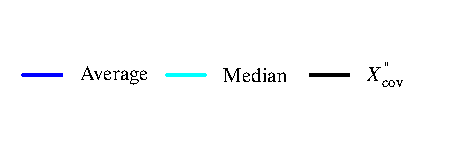
\includegraphics[width=\textwidth]{legendPoints.pdf} % requires the graphicx package
	\vspace{-5em}

                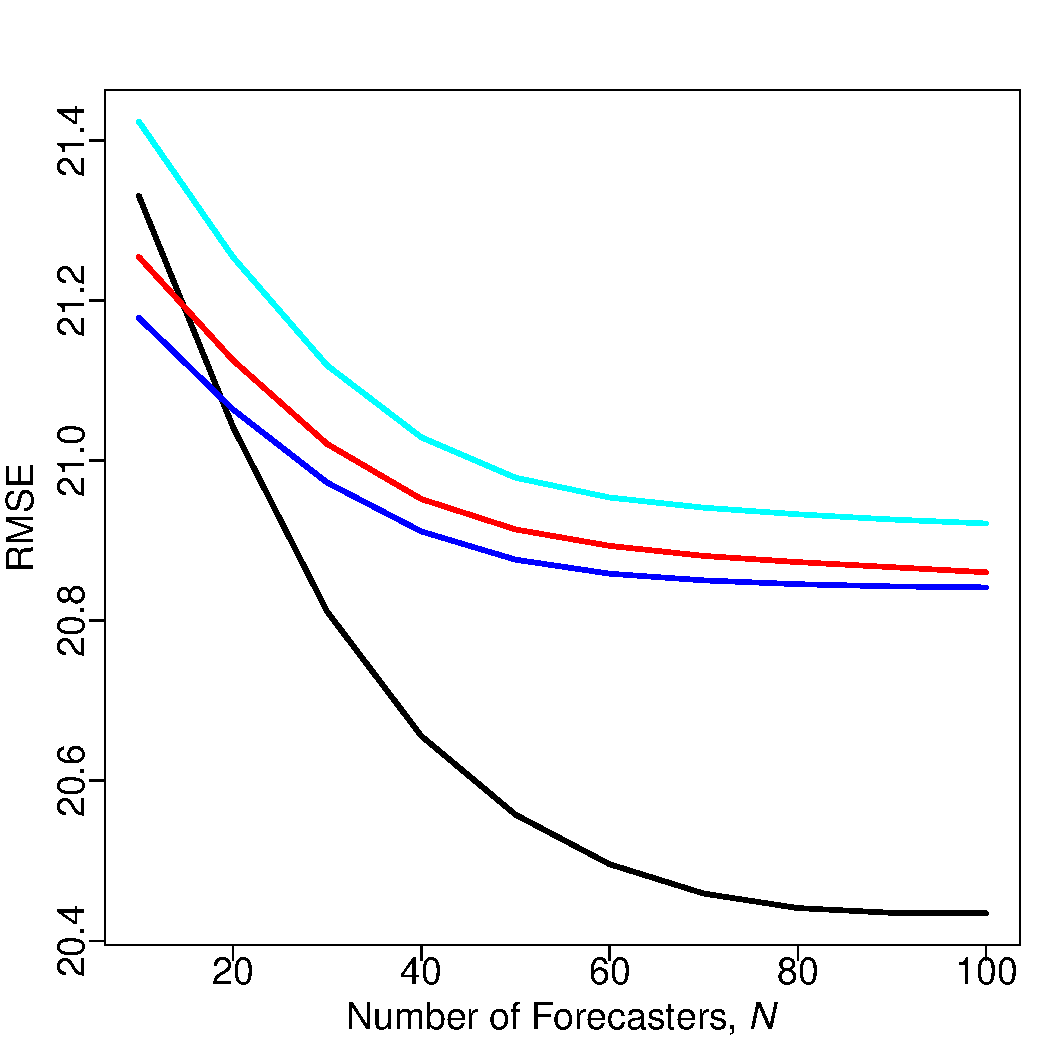
\includegraphics[width=\textwidth]{PointEstimates.pdf}
                \caption{Accuracy of the competing aggregators}
                \label{pointsAcc}
        \end{minipage}%
        %\begin{subfigure}{0.455\textwidth}
        \begin{minipage}[b]{0.495\textwidth}
                 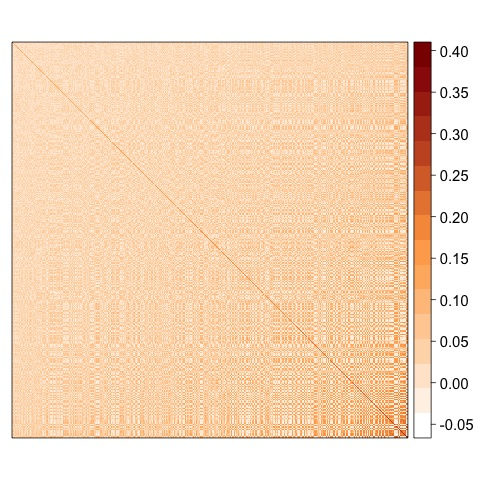
\includegraphics[width=\textwidth]{InfoPlotPoints.jpg}
%	\vspace{0.8em}
            \caption{Information diversity among the 416 participants}
                                \label{ID416}
        \end{minipage}
\end{figure}

\marginpar{This is over a grid of 100 values}

\marginpar{Maybe we should mention that performs poorly under small N because this does not allow tk to be estimated accurately.}

This aggregator is compared against the average and median estimates. Overall accuracy is measured with the RMSE averaged over $10,000$ sub-samplings of the $416$ participants. That is, each iteration chooses $N$ participants uniformly at random, aggregates their forecasts, and computes the RMSE. The size of the sub-samples is varied between $10$ and $100$ with increments of $10$. These scores are presented in Figure \ref{pointsAcc}. Similarly to the synthetic point forecasts in Section \ref{simulation}, the average outperforms the median across all $N$. The revealed aggregator $X_{cov}''$ is the most accurate once $N > 10$. Furthermore, it collects information more efficiently and hence increases the performance advantage as $N$ becomes larger. 

\marginpar{This needs to be said differently; the difference is after all quite impressive.}

Overall, however, the advantage is not as dramatic as in Section \ref{binaryReal}. This is explained by Figure \ref{ID416} that shows $\bSigma_{cov}$ for all the 416 forecasters. The structure has been ordered such that the most knowledgeable forecasters are on the right. This plot is much more monochromatic than the one presented earlier in Figure \ref{top100}, suggesting that information diversity among the 416 students is indeed relatively lower. When information diversity is low, averaging aggregators, such as the simple average, tend to perform relatively well \citep{satopaamodeling}. 

%\marginpar{Try with all 416. See what the results look like}

% As mentioned earlier, the revealed aggregator is not affected by this choice. To make this specific, suppose that $\varepsilon \sigma_0^2$ for some $\varepsilon > 0$ was used instead of $\sigma_0^2$. Then, $\Z \sim \mathcal{N}_N(\boldsymbol{0}, \bSigma/\varepsilon)$ and, by simple cancellation, $X''$ becomes exactly as in (\ref{revPoint}). Of course, for the sake of estimation, some $\sigma_0^2$ must be chosen.






\section{Discussion}
\label{discussion}


\section{Appendix A}
%
%\section{Linking Information and Observations}
%\label{outcomes}
%\marginpar{MAYBE MOVE THIS and explain how to link with the actual data examples.}
%\marginpar{Do not erase but move to appendix.}
%
%This section illustrates the versatility of the Gaussian model by applying it to different types of target quantities. The discussion begins with an easier setup and gets more involved towards the end of the section. In each case, the formulation begins with a careful construction of a known one-to-one mapping between the forecasts and the information variables. This ensures identifiability of the resulting partial information model.
%
%%\subsection{Probability Estimates for Binary Outcomes}
%%Let $A$ denote some future event with two possible outcomes. Suppose the forecasters provide probability forecasts for this event. That is, if $p_i \in [0,1]$ is the probability forecast given by forecaster $i$, then $X_i = p_i$ and $Y = \one_A$. The outcome is linked to the information pool by setting $A = \{Z_S > 0\}$, which suggest a non-informative prior probability of $\P(A) = 1/2$. This can be easily changed to any probability by choosing a different half-space. As this paper is not focused on any particular event, the current choice, however, is the most natural starting point. The forecasts link to the information pool by
%%\begin{align*}
%%p_i &= \P\left(A | \mathcal{F}_{i}\right) = \P\left(Z_S > 0 | Z_{B_i}\right) = \Phi\left( \frac{Z_{B_i}}{\sqrt{1-\delta_i}}\right),
%%\end{align*}
%%where $\Phi(\cdot)$ denotes the CDF of a standard Gaussian distribution. This forecast has a very intuitive marginal distribution. In particular, a forecaster with no information ``withdraws'' from the problem by predicting a non-informative probability $1/2$ while a forecaster with full information always predicts the correct outcome with absolute certainty. 
%%The revealed aggregator is
%%\begin{align*}
%%p'' & =  \P\left(A  | \F''\right) =  \P\left(Z_{S} > 0 | \boldsymbol{Z}\right) = \Phi\left( \frac{{\bf\Sigma}_{12} {\bf\Sigma}_{22}^{-1} \boldsymbol{Z}}
%%   {\sqrt{1 - {\bf\Sigma}_{12} {\bf\Sigma}_{22}^{-1} {\bf\Sigma}_{21}}}\right) 
%%%\label{GeneralAggregator} \,
%%\end{align*}
%
%\subsection{Point Estimates for Continuous Outcomes}
%Suppose that the quantity of interest $Y$ and the predictions $X_j$ are real-valued. Denote the proper non-informative prior distribution with $Y \sim \mathcal{N}(\mu_0, \sigma_0^2)$. The individual forecasts $X_j \sim \mathcal{N}(\mu_j, \sigma_j^2)$, where $\sigma_0^2 \geq \sigma_i^2$; otherwise some forecast is considered less informative than the commonly agreed non-informative prior. Furthermore, the mean of the forecasts $\mu_j = \mu_0$ because the forecasts are assumed to be conditionally unbiased; that is, $\E[Y|X_j] = X_j$. This follows specifically from the conditional distribution $Y | X_j \sim \mathcal{N}(\mu_0 + (X_j - \mu_j), \sigma^2_0 - \sigma^2_j)$. Hence $\E[Y | X_j] = \mu_0 + (X_j - \mu_j)$, which is equal to $X_j$ if and only if $\mu_0 = \mu_j$.  The observables link to the information pool by $Z_S = (Y - \mu_0)/\sigma_0 \sim \mathcal{N}(0,1)$ and $Z_{B_j} = \left(X_j - \mu_0\right)/\sigma_0 \sim \mathcal{N}(0, \delta_j)$, where $\delta_j = \sigma_j^2/\sigma_0^2 \in [0,1]$. If $\Z = \left(Z_{B_1}, \dots, Z_{B_N}\right)'$, then the revealed aggregator is
%\begin{align*}
%X'' =  \E\left(Y  | \F''\right) =  \E\left(Y | \X\right) &= {\bf\Sigma}_{12} {\bf\Sigma}_{22}^{-1} \Z \sigma_0 + \mu_0
%%&= {\bf\Sigma}_{12} {\bf\Sigma}_{22}^{-1} (\boldsymbol{Y} - \mu_S\one) + \mu_S
%%&= {\bf\Sigma}_{12} {\bf\Sigma}_{22}^{-1}\boldsymbol{Y} +\mu_s(1- {\bf\Sigma}_{12} {\bf\Sigma}_{22}^{-1}\one)\\
%\end{align*}
%The current paper applies this model first to simulated data in Section \ref{simulation} and then later on to real-world forecasting data in Section \ref{continuousReal}. 
%
%
%
%
%\subsection{Probability Estimates for  Continuous Outcomes}
%\label{continuous}
%This section assumes that the quantity of interest $Y$ is real-valued, and that the forecasts are in the form of Gaussian distributions. Such a scenario is typical in Bayesian statistics, where multiple researchers working together assign a separate prior distribution on some parameter. The task is then to aggregate these prior distribution in some manner before the posterior distribution can be computed and the statistical analysis carried out. 
%
%%\textcolor{red}{could pick out the most non-informative as the prior}\\
%%\textcolor{red}{how about scaling}\\
%%\textcolor{red}{check informative prior online}
%
%Similarly to the previous subsection, denote the proper non-informative prior with $Y \sim \mathcal{N}(\mu_0, \sigma_0^2)$. The outcome is linked to the information pool by $X_S = (Y-\mu_0)/\sigma_0 \sim \mathcal{N}(0, 1)$. forecaster $j$ reports $\mathcal{N}\left(\mu_j, \sigma^2_j\right)$, where $\sigma_0^2 \geq \sigma_j^2$; otherwise some forecaster is less informated than the commonly agreed non-informative prior. The predictions then link to the information pool via
%\begin{align*}
%Z_{B_j} &= \frac{\mu_j - \mu_0}{\sigma_0} && \text{ and } && \delta_j = 1-\frac{\sigma_j^2}{\sigma_0^2}.
%\end{align*}
% If $\Z = \left(Z_{B_1}, \dots, Z_{B_N}\right)'$, then the revealed aggregator is
%%
%%This restriction illustrates that variance decreases in the amount of information held by the expert. Given that  $\mathcal{N}(\mu_0, \sigma_0^2)$ is the forecast given under no information, the variance of any forecast must be at most $\sigma_0^2$. Now, referring back to (\ref{NExperts}), if $\boldsymbol{X} = (X_{I_1}, X_{I_2},  \dots, X_{I_N})'$ is a column vector of length $N$ and $\Sigma_{22}$ is a coherent overlap structure such that $\Sigma_{22}^{-1}$ exists, then 
%%\begin{align*}
%%X_{S} | \boldsymbol{X} \sim \mathcal{N}\left(\bar{\mu}, \bar{\Sigma}\right), 
%%\end{align*}
%%where
%%\begin{align*}
%%\bar{\mu} &= \mu_1 + \Sigma_{12} \Sigma_{22}^{-1} (\boldsymbol{X} - \boldsymbol{\mu}_2) =  \Sigma_{12} \Sigma_{22}^{-1} \boldsymbol{X} \\
%% \bar{\Sigma}&= \Sigma_{11} - \Sigma_{12} \Sigma_{22}^{-1} \Sigma_{21} =1 - \Sigma_{12} \Sigma_{22}^{-1} \Sigma_{21}  
%%\end{align*}
%%Finally, the aggregate distribution for $Z_S$ is
%\begin{align*}
%Y | \boldsymbol{Z} \sim \mathcal{N}\left(\sigma_0 \bar{\mu} + \mu_0, \sigma_0 \bar{\Sigma}\right),
%\end{align*}
%where $\bar{\mu} =  \diag(\bSigma)' \bSigma^{-1} \boldsymbol{Z}$ and $\bar{\Sigma}=1 - \diag(\bSigma)' \bSigma^{-1} \bSigma_{21}$. Given that $Z_{B_j}$'s and $\delta_j$'s are known to the aggregator, the only unknown quantities are the $\rho_{ij}$'s, namely the information overlap parameters. 
%
%
%
%\subsection{Probability Estimates for Categorical Outcomes}
%
%\begin{figure}[t!]
%   \centering
%   \includegraphics{multinomial} % requires the graphicx package
%   \caption{Illustration of the binary tree that determines the outcome of the event with $M$ possible categorical values.}
%   \label{multinomial}
%\end{figure}
%
%Suppose $Y$ is categorical with $M \geq 2$ potential outcomes $y_1, y_2, \dots, y_M$. The estimate $X_j$ given by forecaster $j$ is a vector of probabilities $\boldsymbol{p}_j = \{p_j^{(1)}, \dots, p_j^{(M-1)}\}  \in \Delta_M$, where $\Delta_M$ is the $M$-dimensional probability simplex. Given that the potential outcomes of $Y$ have no particular ordering to them, the observables must be linked to the information pool symmetrically such that each outcome is positioned identically relative to every other outcome. 
%%This can be formulated in various ways.
%% For instance, the Gaussian process could be extended to a $(M-1)$-dimensional vector with independent coordinates. The $(M-1)$-dimensional space is then partitioned symmetrically into $M$ cones with apexes at the origin. The cone which contains the final value of the Gaussian vector represents the outcome of the event. Another alternative is to consider $M$ independent one-dimensional Gaussian processes and determine the outcome of the event by the maximum (or minimum) of these processes. Even though these approaches may seem reasonable at first, they require solving a system of integral equations in order to map the forecasters' predictions to the information pool. Unfortunately, the integrals involve the Gaussian kernel and must be solved numerically. Therefore, 
%% 
% To construct such a formulation, denote the non-informative prior distribution for $Y$ with $\P(Y = y_m) = q_m$ with $m = 1, \dots, M$.
%%be uniform over the $C$ outcomes; that is, $\P(Y = y_k) = 1/K$ for $k = 1, \dots, K$. 
%Extend the Gaussian process to $M-1$ dimensions:
%\begin{align*}
% \left\{\Z_\B = \left(Z_{B_1}^{(1)}, Z_{B_2}^{(2)},  \dots, Z_{B_{M-1}}^{(M-1)}\right)' \in \mathbb{R}^{M-1} \right\},
% \end{align*}
% where the coordinates are independent Gaussian processes (as defined by the Gaussian Information Pool; see Section \ref{gaussian}) and $\B = (B_1, \dots, B_{M-1}) \subseteq \boldsymbol{S} = [0,1]^{M-1}$. The final value of $Y$ is determined by descending through a binary tree illustrated in Figure \ref{multinomial}. Each leaf node represents a different outcome of $Y$. The $m$th branch down is taken if $Z_{S}^{(m)}$ is higher than  
% \begin{align*}
%t_m &= \begin{cases}
%\Phi^{-1}\left[1-q_m\right] & \text{ if } m = 1\\
%\Phi^{-1}\left[1-\frac{q_m}{\prod_{h=1}^{m-1} (1-q_h)} \right] & \text{ if } m \in \{2, \dots, M-1\}
%\end{cases}
% \end{align*}
% These thresholds follow directly from the prior distribution and the fact that $Z_{S}^{(m)} \stackrel{i.i.d.}{\sim} \mathcal{N}(0,1)$ for $m = 1, \dots, M-1$. 
%%
%% The coordinate $Z_{S_m,m}$ is associated with the node above outcome $y_m$. To make this more precise, define 
%%\begin{align*}
%%q_k &= \begin{cases}
%%\Phi^{-1}\left[(K-1)/K\right] & \text{ if } k = 1\\
%%\Phi^{-1}\left[1-(K-1)^{1-k}K^{k-2} \right] & \text{ if } k \geq 2
%%\end{cases}
%%\end{align*}
%%The path then branches downwards at the $k$th node if the event 
%
%
%forecaster $j$ then makes a probability estimate for $Y$ conditional to observing $\Z_{\B_j}$ for some $\B_j = (B_{1,j}, \dots, B_{M-1,j})  \subseteq \boldsymbol{S}$. First, let $A_m = \left\{ Z_{S}^{(m)} > t_m\right\}$ denote the event of branching downward at the $m$th parent node and define $r_{j,m}$ to be forecaster $j$'s probability estimate for $A_m$. Then, 
%\begin{align}
%r_{j}^{(m)}  := \P\left(A_m | \F_{j}^{(m)}\right) = \Phi\left( \frac{Z_{B_{m,j}}^{(m)} - t_m}{\sqrt{1-\delta_{j}^{(m)}}}\right),\label{branch}
%\end{align}
%where $\delta_{j}^{(m)} = |B_{m,j}|$ represents the amount of information that forecaster $j$ has about outcome $y_m$. These branching probability estimates relate to the actual probability forecasts via the following one-to-one, recursive mapping
%\begin{align}
%\label{categ_aggre}
%p_{j}^{(m)} = \P\left(Y = y_k | \Z_{\B_j} \right) &= \begin{cases}
%r_{j}^{(m)} & \text{ if } m = 1\\
%r_{j}^{(m)} \prod_{h=1}^{m-1}\left(1-r_{j}^{(h)} \right)  & \text{ if } m \in \{2, \dots, M-1\}
%\end{cases}
%\end{align}
%There are two observations worth emphasizing: a) given the prior distribution and the forecaster's level of information, (\ref{branch}) and (\ref{categ_aggre}) establish a simple, one-to-one mapping between the probability forecast $p_{j}^{(m)}$ and the information variable $Z_{S}^{(m)}$; and b) 
%%This establishes a one-to-one, recursive mapping between $\{r_{i,k} : k = 1, \dots, K-1\}$ and $\{p_{i,k} : k = 1, \dots, K-1\}$.  
%%Note that the above model reduces to the binary case when $K = 2$. Similarly to the binary case, 
%the probability forecasters exhibit very intuitive behavior. In particular, $p_{j}^{(m)}$ is marginally uniform over the vertices of the $M$-simplex when $\delta_{j}^{(m)} = 1$ for all $m = 1, \dots, M-1$.  The marginal distribution converges to a point mass at the non-informative prior distribution as $\delta_{j}^{(m)} \to 0$.  This ``point of ignorance" has been acknowledged previously in the literature (see, e.g., \citealt{fox2003partition, see2006between, satopaa}). Therefore a forecaster with no information ``withdraws'' from the problem by predicting a non-informative distribution while a forecaster with full information always predicts the correct outcome with absolute certainty. 
%
%To derive the revealed aggregator, collect the $m$th coordinates of the forecasters' information variables into a vector $\Z^{(m)} = \left(Z_{B_{m,1}}^{(m)}, Z_{B_{m,2}}^{(m)}, \dots, Z_{B_{m,N}}^{(m)} \right)'$. The extended vector  $\left(Z_{S_m}, \Z^{(m)} \right)'$ then follows a $(N+1)$-dimensional (centered) Gaussian distribution with 
%%This specifies the following joint distribution for the random variables in the model:
%%\begin{align*}
%%f\left(\left\{ \Z^{(m)} \right\}_{m=1}^{M-1} \bigg| \left\{ \bSigma^{(m)} \right\}_{m=1}^{M-1}  \right) &= \prod_{m=1}^{M-1} f_{N+1}\left(\Z^{(m)} | \bSigma^{(m)}\right), 
%%\end{align*}
%%where $f_N(\cdot | \bSigma)$ denotes the PDF of an $N$-dimensional multivariate Gaussian with covariance matrix $\bSigma$. 
%a covariance matrix
%\begin{align*}
%\bSigma^{(m)} &=
%\left(\begin{matrix} 
%1& {\bf \Sigma}_{12}^{(m)}\\
%{\bf \Sigma}_{21}^{(m)} & {\bf \Sigma}_{22}^{(m)}\\
% \end{matrix}\right),
%\end{align*}
%where ${\bf \Sigma}_{21}^{(m)} = {{\bf \Sigma}_{12}^{(m)}}' = \diag\left(\bSigma^{(m)}\right)$.
%%The $j$th agent then observes some portion $I_{j,k}$ of the process $X_{S,k}$. Represent this information with $X_{I_{j,k}}$, where $|I_{j,k}| = \delta_{j,k}$. If the information overlap between agents $i$ and $j$ about split $k$ is denoted with $\rho_{ij,k} = |I_{i,k} \cap I_{j,k}|$, then the multivariate Gaussian distribution becomes 
%%\begin{align*}
%%\left(\begin{matrix} \boldsymbol{X}_S \\ \boldsymbol{X}_1\\ \vdots \\ \boldsymbol{X}_{K-1} \end{matrix}\right) &\sim \mathcal{N}_{}\left( 
%% \boldsymbol{0}, 
%%% \left(\begin{matrix} 
%%%\Lambda_{11} & \Lambda_{12}\\
%%%\Lambda_{21} & \Lambda_{22}\\
%%% \end{matrix}\right) 
%%% =
%% \left(\begin{array}{c c c c | c c c c c}
%%  \multicolumn{4}{c|}{\multirow{4}{*}{$I_{K-1}$}} & \Sigma_{12,1}  & &  \multicolumn{2}{c}{\multirow{2}{*}{$\boldsymbol{0}$}}   \\ 
%% & &  & & &  \Sigma_{12,2} && & \\ 
%%   &  &  &  &  \multicolumn{2}{c}{\multirow{2}{*}{$\boldsymbol{0}$}}  & \ddots&  \\ 
%%   &  &  &  &&& &\Sigma_{12,K-1}  \\ \hline
%%\Sigma_{21,1} & &\multicolumn{2}{c|}{\multirow{2}{*}{$\boldsymbol{0}$}}& \Sigma_{22,1} & & \multicolumn{2}{c}{\multirow{2}{*}{$\boldsymbol{0}$}}   \\ 
%% & \Sigma_{21,2} & & &  & \Sigma_{22,2} &&  \\ 
%%\multicolumn{2}{c}{\multirow{2}{*}{$\boldsymbol{0}$}}& \ddots &&\multicolumn{2}{c}{\multirow{2}{*}{$\boldsymbol{0}$}}  & \ddots &  \\ 
%%&&  & \Sigma_{21,K-1} &  &  &&\Sigma_{22,K-1} \\ 
%% \end{array}\right)\right),
%%\end{align*}
%%where
%%\begin{align*}
%%%\Sigma_{21,k} &= \Sigma_{12,k}' = \left(\begin{matrix} \delta_{1,k} \\ \delta_{2,k} \\ \vdots \\ \delta_{N,k} \end{matrix}\right) && 
%%\bSigma_{22,k} =  \left(\begin{matrix}
%%\delta_{1,k} &\rho_{12,k} & \dots & \rho_{1N,k}   \\ 
%% \rho_{21,k} & \delta_{2,k} & \dots & \rho_{2N,k}  \\ 
%% \vdots & \vdots & \ddots & \vdots  \\ 
%% \rho_{N1,k} & \rho_{N2,k} & \dots & \delta_{N,k}\\ 
%% \end{matrix}\right) 
%%\end{align*}
%The covariance matrix $\bSigma^{(m)}$ is akin to the one described in (\ref{NExperts}) and represents the forecasters' information structure associated with the $m$th outcome $y_k$. 
%%Therefore the information structure can vary among different outcomes of $Y$. Of course, different variations are possible. 
%The branching probabilities $r_{j}^{(m)}$ can be then aggregated separately at each parent node. That is, if
%\begin{align*}
%r^{(m)}_{rev} & = \P\left(A_m | {\F}_{rev}^{(m)}\right)   = \Phi\left( \frac{\diag(\bSigma)'^{(m)} {\bSigma^{(m)}}^{-1} \boldsymbol{Z}^{(m)} - t_m}
%   {\sqrt{1 - {\diag(\bSigma)'^{(m)} {\bSigma^{(m)}}^{-1} {\bSigma}_{21}^{(m)}}}}\right),
%%\label{probAggre}
%\end{align*}
%the revealed aggregates $p_{rev}^{(m)}$ are obtained by replacing $r_{j}^{(h)}$ in (\ref{categ_aggre}) with $r^{(m)}_{rev}$. 
%%The form (\ref{probAggre}) has an interesting interpretation: Given the forecasters' information, the numerator is the best point estimate of $Z_{S}^{(m)}$. This is then extremized, i.e., transformed away from $t_m$ depending on how much the entire group of forecasters know. Their amount of information is estimated with ${\diag(\bSigma)'^{(m)} {\bSigma^{(m)}}^{-1} {\bSigma}_{21}^{(m)}} \in [0,1]$. Therefore, the more they know, the further away the point estimate is transformed from $t_m$ and then closer the probability $r^{(m)}_{rev}$ is to zero or one. Extremization has been widely studied in literature. 
%Observe that if $M = 2$, the subindex $m$ can be dropped, simplifying the expressions largely. Such a binary outcome is definitely the most common sub-case encountered in practice. See \cite{satopaamodeling} for a detailed discussion of the Gaussian model under binary outcomes. This aggregator is re-visited in Section \ref{binaryReal} that applies it to a set of real-world forecasts on different geopolitical events. 
%
%\marginpar{It is not good to change the notation of the revealed aggregator}
%
%
%%\marginpar{Talk about the interpretation of the aggregation formula: denim and numerator. Automatic extremization.}
%%
%%\marginpar{Reference the other paper for the C=2 case}
%
%
%%\marginpar{ add the revealed aggregator}
%
%%If the experts' information sets are non-overlapping, the information structures $\left\{\Sigma_{22, k}\right\}_{k=1}^K$ are diagonal and the experts' forecasts are independent. By assuming independent forecasts and conditioning on a particular outcome $\boldsymbol{X}_S = \boldsymbol{x}$ reveals that the conditional covariance of any two experts' information is $\text{cov}(X_{I_{i,k}, k}, X_{I_{j,k}, k} | \boldsymbol{X}_S = \boldsymbol{x}) = -\delta_{i,k}\delta_{j,k} \leq 0$. The mapping from $\left\{X_{I_{j,k}, k}\right\}_{k=1}^K$ to $\left\{p_{j, k}\right\}_{k=1}^K$ sustains the negative covariance. Therefore, as long as  both experts' hold some information, i.e. $\delta_{i,k}, \delta_{j,k} > 0$, any two independent forecasts are negatively correlated conditional the outcome of the event. This is one of the core statistical properties of independent interpreted estimates (\cite{hong2009interpreted}).
%

%\subsection{Probability model of information}

%\marginpar{This is not correct; much work needed.}
%
%forecaster $i$ with no information reports a non-informative prediction given by the prior expectation; that is, if $\mathcal{F}_i =\{\emptyset, \Omega\}$, then $X_i = \E(Y)$. On the other hand, if forecaster $i$ uses all the information,  $X_i$ is a point mass at the correct value of $Y$; that is, if $\mathcal{F}_i = \mathcal{F}$, then $X_i = \E(Y|\mathcal{F}) = Y$.  These logical extremes characterize the forecasters' behavior at different levels of information, and the distance to the non-informative forecast facilitates estimation of the forecaster's amount of information. 
%
%Estimation of the latter quantity, on the other hand, relies on the correlation of the forecasts. To make this more specific, recall that two $\sigma$-algebras $\mathcal{F}_i$ and  $\mathcal{F}_j$ are called independent if for all $B \in \mathcal{F}_i$ and $C \in \mathcal{F}_j$ the events $B$ and $C$ are independent, i.e. $\P(B \cap C) = \P(B) \P(C)$. In other words, $\mathcal{F}_i$ does not provide any additional information about $\mathcal{F}_j$, and \textit{vice versa}. Therefore independent $\sigma$-fields can be considered \textit{informationally disjoint}. Given that $X_j$ is measurable with respect to $\mathcal{F}_j$,  forecasts based on informationally disjoint sets are independent and hence uncorrelated. At the other extreme, if $\mathcal{F}_i = \mathcal{F}_j$, the forecasts $X_i$ and $X_j$ are the same and have a perfect positive correlation.  Therefore it is reasonable to assume that the correlation between any two forecasts increases in size of the forecasters' information overlap. 

\subsection{Proof of Proposition \ref{covstr}}

\begin{proof} 
Denote the common marginal mean with $\mu = \E[X_j]$ for all $j = 1, \dots, N$. Each item is then proved as follows.
\begin{enumerate}[i)]
\item Given that $\E[Y | X_j]  = X_j$, the law of iterated expectation gives $\E[\E[Y | X_j]]  = \E[Y] = \E[X_j]$ for all $j = 1, \dots, N$. 
\item This follows from direct computation:
\begin{align*}
\Cov(X_j, X_i) &= \E[(X_j - \mu)(X_i - \mu)]\\
&= \E[X_jX_i] - \mu^2\\
&= \E[\E[X_j|X_i]X_i] - \mu^2\\
&= \E[\E[\E[Y|X_j]|X_i]X_i] - \mu^2\\
&= \E[\E[Y|X_i]X_i] - \mu^2\\
&= \E[X_i^2] - \mu^2\\
&= \Var(X_i)
\end{align*}
\item This follows from item ii) and an application of the Cauchy-Schwarz inequality:
\begin{align*}
\Var(X_i) &= \Cov(X_i, X_j)\\
&= \E[(X_i - \mu)(X_j - \mu)]\\
&\leq \E[(X_i - \mu)^2]^{1/2}\E[(X_j - \mu)^2]^{1/2}\\
&= \sqrt{\Var(X_i) \Var(X_j)},
\end{align*}
which then provides $\Var(X_i) \leq \Var(X_j)$. This inequality is tight because $X_i = X_j$ for $\F_i = \F_j$. 

\end{enumerate}
\end{proof}


%\subsection{Proof of Proposition \ref{synth}}
%\begin{proof}
%%It is helpful to first establish membership in what is typically known as the correlation polytope $\COR_N :=  \conv\left\{
%%\boldsymbol{x}\boldsymbol{x}' : \boldsymbol{x} \in
%%\{0,1\}^N\right\}$. 
%Begin by approximating the full information with a finite set of $L$ elements. Describe the $j$th forecaster's information with a binary vector $\v_j$ whose $L$ entries indicate which elements of the full information the forecaster knows. Suppose this vector is constructed by making $L$ independent draws from a Bernoulli distribution with success probability $\delta_j \in [0,1]$. Let $\v_0 = \one$ be of a vector of $L$ ones. If $\V$ is a $(N+1) \times L$ matrix with the $k$th row equal to $\v_{k-1}/\sqrt{L}$, the corresponding Gramian matrix $\V \V' $ is always in $ \mathcal{S}_{+}^{N+1}$. Given that $\mathcal{S}_{+}^{N+1}$ is a convex set, the expectation of  $\V \V' $ is also in $\mathcal{S}_{+}^{N+1}$. The diagonal and off-diagonal elements of this expectation are the desired $\E[\v_j' \v_j/L] = \delta_j$ and $\E[\v_i' \v_j/L] = \delta_i \delta_j$, respectively.  
%%Finally, \cite{laurent1997connections} showed that all $\bSigma \in \COR_N$ satisfy $h(\bSigma) \in \mathcal{S}_{+}^{N+1}$. 
%\end{proof}


\subsection{Finding $\mu^*$ for $\mathcal{P}_{sd}(\cdot : \kappa)$} 
 \begin{algorithm}[t!]
\caption{This procedure solves (\ref{globalMu}) efficiently using the structure of the problem and binary-search.} 
\label{projSD_algo}
\begin{algorithmic}[1]
\Require $\kappa \geq 1$ and sample eigenvalues in ascending order $\l_1 \leq l_2 \leq \dots \leq l_{N+1}$.
\Procedure{binary-search optimization}{}
\State Initialize $D \leftarrow \max\{l_1,0\}$ and  $U \leftarrow l_{N+1}/\kappa$.
\State $\mu_0 \leftarrow (D + U)/2$
%\State $\bLambda_{lin} \leftarrow \boldsymbol{0}$
%\State $\bSigma_{cond} \leftarrow \mathcal{P}_{cond}(h(\boldsymbol{S}_Z) : \kappa)$.
\For{$n = 0, 1, \dots$}
\State Compute $\mu_n^*$, $\mathfrak{d}_n$, and $\mathfrak{u}_n$. 
\If {$\mu_n^* < 0$ and $\mathfrak{d}_n < 0$}
\State \Return $0$ 
\ElsIf{$\mu_n^* < \mathfrak{d}_n$}
\State $U \leftarrow \mathfrak{d}_n$
\ElsIf{$\mu_n^* > \mathfrak{u}_n$}
\State $D \leftarrow \mathfrak{u}_n$
\Else 
\State \Return $\mu_n^*$
\EndIf
\State $\mu_{n+1} \leftarrow (D + U)/2$
\EndFor
\State \Return $\mu_n^*$
\EndProcedure
\end{algorithmic}
\label{algo}
\end{algorithm}


This section describers a binary-search-like algorithm to solve
\begin{align}
\mu^* = \argmin_{\mu \geq 0 }g(\mu) &=\argmin_{\mu \geq 0 }\sum_{i=1}^{N} \left[ \left(\mu-l_i\right)^2_+ + \left(l_i - \kappa\mu\right)^2_+ \right] \label{globalMu}
\end{align}
First, it can be assumed that $\cond(h(\SS_Z)) \notin [0,\kappa]$; otherwise, the projection can simply return $h(\SS_Z)$. Second, $\max\{0, l_1\} \leq \mu \leq l_{N+1}/\kappa$ because otherwise moving $\mu$ closer to the nearest sample eigenvalue decreases $g(\mu)$. Now, consider some value $\mu_n \geq 0$ and two index sets $\mathfrak{D}_n = \{i : l_i \leq \mu_n\}$ and $\mathfrak{U}_n = \{i : \mu_n\kappa \leq  l_i \}$. Then,
\begin{align*}
g(\mu_n) &= \sum_{i \in \mathfrak{D}_n}  \left(\mu_n-l_i\right)^2  + \sum_{i \in \mathfrak{U}_n} \left(l_i - \kappa\mu_n\right)^2,
\end{align*}
 which has a global minimum at 
\begin{align*}
\mu_n^* &= \frac{\sum_{i \in \mathfrak{D}_n} l_i  + \kappa \sum_{i \in \mathfrak{U}_n} l_i }{|\mathfrak{D}_n | + \kappa^2 |\mathfrak{U}_n|}
\end{align*}
 The operator $|\mathfrak{A}|$ denotes the number of elements in the set $\mathfrak{A}$.  Let $\mathfrak{d}_n$ and $\mathfrak{u}_n$ denote the minimum and maximum, respectively, of the interval where any value of $\mu$ gives the index sets $\mathfrak{D}_n$ and $\mathfrak{U}_n$. To make this specific, define two operators:
 \begin{align*}
 d(\mu) = \max\{l_i : l_i \leq \mu\} &&& \text{ and } &&& u(\mu) = \min\{l_i : l_i \geq \mu\}.
\end{align*} 
If no value is found, then $d(\mu) = 0$ and $u(\mu) = +\infty$.  Then, 
 \begin{align*}
\mathfrak{d}_n &= \max \{d(\mu_n), d(\mu_n\kappa)/\kappa\}\\
\mathfrak{u}_n &= \min \{u(\mu_n), u(\mu_n\kappa)/\kappa\}
\end{align*}
 Of course, $\mu^*_n$ is the solution to (\ref{globalMu}) as long as $\mu_n^* \in [\mathfrak{d}_n, \mathfrak{u}_n]$. If, on the other hand, $\mu_n^*$ is less than $\mathfrak{d}_n$ (or greater than $\mathfrak{u}_n$), the global minimum $\mu^*$ must be smaller than $\mathfrak{d}_n$ (or greater than $\mathfrak{u}_n$). If $\mu_n^*$ is, say, less than $\mathfrak{d}_n$, then a natural approach is to update $\mu_n$ to $\mu_{n+1}$ that is somewhere between $\mathfrak{d}_n$ and some known lower bound of $\mu$.  This gives rise to a binary-search-like algorithm described in Algorithm \ref{projSD_algo}. 
 
% To show that this algorithm converges, it is enough to prove that $U
 
% The next proposition guarantees that the algorithm converges.
% 
% \begin{proposition}
% Algorithm 
% \end{proposition}
% 

% \marginpar{Proof convergence by showing the UPB-LWB decreases every iteration.}
 

%\subsection{Maximum Likelihood Estimation}
%%The initial problem can be rewritten as
%%\begin{align}
%%\label{mle}
%%\begin{split}
%%\text{minimize } & \sum_{i=1}^N l_i/\lambda_i + \log(\lambda_i) \\
%%\text{subject to } & 0 \leq u \leq \lambda_i \leq \kappau, \text{   } i = 1, \dots, N
%%\end{split}
%%\end{align}
%
%%\marginpar{No need to do this. MLE overfits. Use regular gradient descent.}
%
%%
%%
%%\marginpar{Explain somewhere how to extend this to transformations of the variable.}
%%
%%\marginpar{$\delta$ is a weighted sum of the eigenvalues.}
%%
%To reduce the dimension of the estimation problem, compute the spectral decomposition $\SS_Z = \Q \L \Q'$ with $\L = \Diag(l_1, \dots, l_N)$. \citet{won2006maximum} showed that minimizing the negative log likelihood with respect to $\bSigma$ is equivalent to finding the eigenvalues $\lambda_1, \dots, \lambda_N$ that minimize $ \sum_{i=1}^N (l_i/\lambda_i + \log \lambda_i)$
%%\begin{align}
%%\text{minimize } &  \sum_{i=1}^N (l_i/\lambda + \log \lambda) \label{convexEigen}
%%\end{align}
% and then setting $\bSigma^{*} = \Q \Diag(\lambda_1^*, \dots, \lambda_N^*)\Q'$. Therefore, the final solution has the same eigenvectors as the sample covariance matrix, but the eigenvalues have been transformed. 
% % After this point, the penalty term is small and the regularized dominates such that $f_i$ resembles the log-function. 
%% The unconstrained solution to (\ref{convexEigen}) is $r_i^* = 1/l_i$ which, as expected, gives $\Sigma_{22}^* = \SS_Z$. 
%% 
%To make use of this, the feasible region must also be expressed in terms of the eigenvalues.
%First, both positive semi-definiteness and an upper bound on the condition number can be enforced 
%%Given that the variables of (\ref{convexEigen}) are the eigenvalues of the final estimate of $\bSigma^{-1}$, positive semi-definiteness and the condition number constraint can be easily included. More specifically, this is done
%by introducing an auxiliary variable $u$ such that $0 < u \leq \lambda_i \leq u \kappa$. Furthermore, the semidefinite relaxation can be expressed in terms of the eigenvalues. Denote the $i$th column of $\Q$ with $\q_i$. If $\widetilde{\Q}$ is an $N\times N$ matrix whose $i$th column is $\diag(\q_i \q_i')$, the diagonal $\diag(\bSigma) = \widetilde{\Q} \blambda$. Then,
% \begin{align*}
%\diag(\bSigma)'  \bSigma^{-1} \diag(\bSigma) &= \blambda \widetilde{\Q}' \Q \Diag(1/\blambda) \Q'  \widetilde{\Q} \blambda\\
%&= \sum_{i=1}^N 1/\lambda_i (\q_i' \widetilde{\Q} \blambda)^2,
%\end{align*}
%which is a convex function of $\blambda$.
%% Given that all the constraints are convex, an attractive alternative would be to replace the objective with a convex relaxation.
%%Unfortunately, this is not a convex function in $\r$. It is, however, convex in $\lambda_i = 1/r_i$, which are the eigenvalues of the final estimate of $\bSigma$. Under this change of variable, the semidefinite relaxation becomes $\sum_{i=1}^N (1/\lambda_i) (\q_i' \widetilde{\Q} \blambda)^2 \leq 1$. 
%%The problem is that (\ref{convexEigen}) does not remain convex after the change of variables $r_i = 1/\lambda_i$. 
%%Making the change of variables $r_i = 1/\lambda_i$ in (\ref{convexEigen}) gives
%%\begin{align}
%%\text{minimize } &  \sum_{i=1}^N (l_i/\lambda_i + \log \lambda_i) \label{nonconvexEigen}
%%\end{align}
%%This objective is separable with components $f_i(\lambda_i) = l_i/\lambda_i + \log \lambda_i$. Each $f_i$ can be viewed as the sum of a penalty $\l_i / \lambda_i$ and a regularizer $\log\lambda_i$. Given that the penalty term is convex while the regularizer is concave, $f_i$ is not guaranteed to be convex. In fact, $f_i$ is convex if and only if $\lambda_i \leq 2l_i$. After this point, the penalty term is small and the regularized dominates such that $f_i$ resembles the log-function. The objective (\ref{nonconvexEigen}) is unimodal with the global maximum at $\lambda_i^* = l_i$ which, as expected, gives $\Sigma_{22}^* = \SS_Z$. 
%%Quasiconvex objectives under convex constraints can be solved by a sequence of convex optimization problems. 
%%Given that this approach is likely to be very slow, we introduce a piece-wise convex upper bound for $f_i$:
%%\begin{align*}
%%\tilde{f}(\lambda_i) &= \begin{cases}
%%f(\lambda) & \text{ if } \lambda_i \leq 2\l_i\\
%%\lambda_i/(4l_i) + \log(2l_i) & \text{ otherwise}
%%\end{cases}
%%\end{align*}
%%This convex relaxation follows $f_i$ until $\lambda_i \leq 2l_i$ but then turns into a tangent line to $f_i$ at the point $\lambda_i = 2l_i$. Given that $f_i$ is concave when $\lambda_i > 2l_i$, it is upper bounded by any tangent line. Therefore, $f(\lambda_i) \leq \tilde{f}(\lambda_i)$ and, consequently, $\sum_{i} f_i(\lambda_i) \leq \sum_{i} \tilde{f}_i(\lambda_i)$ for all $\lambda_i \geq 0$. To further motivate $\tilde{f}_i$, observe that $\sum_{i} \tilde{f}_i(\lambda_i)$ also has a unique global minimum at $\lambda_i^* = l_i$. Therefore, if $\SS_Z$ is in within the feasible region, both the original objective (\ref{nonconvexEigen}) and its convex relaxation lead to the same solution.  If, however, $\SS_Z$ is not in the feasible region, then estimation procedure aims to find a feasible solution that is the closest to $\SS_Z$, with closeness defined by the objective. The original and the relaxed objectives differ only if $\lambda_i > 2l_i$ for some $i$. For large $\lambda_i$, however,   $f_i(\lambda_i)$ is well approximated with a linear function. Therefore the contours of the objective can be expected to present similar patterns and, consequently, lead to similar solutions. 
%The MLE of $\bSigma$ is then found by first solving
%\begin{align}
%\label{mle_problem}
%\begin{split}
%%\text{minimize } &  || \bSigma - \boldsymbol{S}_Z ||_F^2 \label{orig_problem}\\
%\text{minimize } &  \sum_{i=1}^N (l_i/\lambda_i + \log \lambda_i)\\
%\text{subject to } & 0 < u \leq \lambda_i \leq \kappau, \hspace{2em} (i = 1, \dots, N)\\
%& \sum_{i=1}^N (1/\lambda_i) (\q_i' \widetilde{\Q} \blambda)^2 \leq 1
%\end{split}
%\end{align}
%with variables $u$ and $\lambda_i$ for $i = 1, \dots, N$, and then computing $\Q \Diag(\lambda_1^*, \dots, \lambda_N^*)\Q'$. Note that the number of variables has been reduced from $\binom{N+1}{2}$ to $N+1$. 
%
%This objective is unimodal with the global maximum at $\lambda_i^* = l_i$ which, as expected, gives $\Sigma_{22}^* = \SS_Z$. Furthermore, the objective is separable with components $f_i(\lambda) = l_i/\lambda + \log \lambda$. This can be viewed as the sum of a penalty $\l_i / \lambda$ and a regularizer $\log\lambda$. Given that the penalty term is convex while the regularizer is concave, $f_i$ is not guaranteed to be convex. In fact, $f_i$ is convex if and only if $\lambda \leq 2l_i$. Therefore a unique solution can be guaranteed by including the additional constraint $\lambda_i \leq 2l_i$ for all $i = 1, \dots, N$. This constraint combined with an upper bound on the condition number, however, can result into an empty feasible region. For instance, if the number of problems is fewer than the number of forecasters, at least one of the eigenvalues of $\SS_Z$ is zero. By constraining $\lambda_i \leq 2l_i$ for all $i = 1, \dots, N$ would then lead to a singular estimator, i.e. an estimate with a condition number equal to positive infinity. 
%
%Observe that if $\SS_Z$ is in the feasible region, the solution to (\ref{mle_problem}) is $\SS_Z$. On the other hand, if $\SS_Z$ is not in the feasible region, the final estimate is the feasible solution that is as close (in terms of the objective) to $\SS_Z$ as possible. The negative log-likelihood was motivated by the underlying Gaussian model but other measures of closeness can be considered. In particular, similar yet convex objectives appear attractive. Given that the current objective is not convex due to the regularizer, it is natural to replace the term $\log(\lambda)$ with a good convex approximation. Although many choices are possible, in some sense the closest such approximation is the tangent line at some point $\lambda_0$.  This gives $\tilde{f}_i(\lambda | \lambda_0) = l_i/\lambda + \log(\lambda_0) + (\lambda - \lambda_0)/\lambda_0$ a majorizing function of $f_i(\lambda)$; that is, $\tilde{f}_i(\lambda | \lambda_0) \geq f_i(\lambda)$ for all $\lambda$, and $\tilde{f}_i(\lambda_0 | \lambda_0) = f_i(\lambda_0)$. This suggests the following majorization-maximization (MM) sub-problem:
%\begin{align}
%\label{mle_problem}
%\begin{split}
%%\text{minimize } &  || \bSigma - \boldsymbol{S}_Z ||_F^2 \label{orig_problem}\\
%\text{minimize } &  \sum_{i=1}^N \left( l_i/\lambda_i^{(t)} + \lambda_i^{(t)}/\lambda_i^{(t-1)} \right)\\
%\text{subject to } & 0 < u \leq \lambda_i^{(t)} \leq \kappau, \hspace{2em} (i = 1, \dots, N)\\
%& \sum_{i=1}^N \left(1/\lambda_i^{(t)}\right) \left(\q_i' \widetilde{\Q} \blambda^{(t)}\right)^2 \leq 1
%\end{split},
%\end{align}
%where $\lambda^{(t-1)}$ is the solution from the previous iteration. 
%The global solution to each MM sub-problem can be found efficiently with standard techniques such as the interior point methods. These have the attractive property of non-decreasing the original objective. Once the MM procedure has converged, the final estimate of $\bSigma$ is then given by $\Q \Diag(\blambda^*)\Q'$. This is not guaranteed to be a global optimum of the original objective. However, the limit points have been shown to be critical points of the original objective. 

%\marginpar{a) may have to add some to $l_i$; b) may have to prove the Lipshitz constant, which should be much easier for this function. }



%The next subsection explores another popular distance measure, namely the class of matrix norms. Given that all matrix norms are convex, this leads to estimation procedures where the global optimum can be found efficiently.  

%
%
%In some sense and especially for large $\lambda$, the closest such approximation is a linear function. Furthermore, given that the relaxed objective should have the same global optimum as the original objective, the penalty term must also be modified. This gives $\tilde{f}_i(\lambda) = l_i^2/\lambda + \lambda$ as a convex approximation of $f_i(\lambda)$, and the corresponding relaxed MLE problem is
%\begin{align}
%\label{mle_problem}
%\begin{split}
%%\text{minimize } &  || \bSigma - \boldsymbol{S}_Z ||_F^2 \label{orig_problem}\\
%\text{minimize } &  \sum_{i=1}^N (l_i^2/\lambda_i + \lambda_i)\\
%\text{subject to } & 0 < u \leq \lambda_i \leq \kappau, \hspace{2em} (i = 1, \dots, N)\\
%& \sum_{i=1}^N (1/\lambda_i) (\q_i' \widetilde{\Q} \blambda)^2 \leq 1
%\end{split}
%\end{align}
%The global solution $\blambda^{*}$ to this problem can be found efficiently with standard techniques such as the interior point methods. The final estimate of $\bSigma$ is then given by $\Q \Diag(\blambda^*)\Q'$. The next subsection explores another popular distance measure, namely the class of matrix norms. Given that all matrix norms are convex, this leads to estimation procedures where the global optimum can be found efficiently.  
%
%
%  Similarly, decompose $\bSigma = \R \Lambda \R'$ with $\R$ orthonormal and $\Lambda = \Diag(\lambda_1, \dots, \lambda_N)$. If $\R = \Q$, then 
%



%Our goal is to solve
%
%\begin{align*}
%\text{minimize } & || \Sigma - S ||_F^2\\
%\text{subject to } & \Sigma \succeq 0\\
% & \text{cond}(\Sigma) \leq \kappa\\
% & \text{Tr}(A_i \Sigma) = a_i, i = 1, \dots, K\\
% & \text{Tr}(B_j \Sigma) \leq b_j, j = 1, \dots, M
%\end{align*}
%Let $S = P Diag(\hat{\lambda}) P'$ be the spectral decomposition of $S$. This problem can be transformed into the following equivalent problem.
%\begin{align*}
%\text{minimize } & || \lambda -  \hat{\lambda}||_2^2\\
%\text{subject to } & -\mu \preceq 0\\
%& \mu - \lambda \preceq 0\\
%& \lambda - \kappa \mu \preceq 0\\
% & A \lambda - a= 0\\
% & B \lambda -b \preceq 0,
%\end{align*}
%where the $i$th row of $A$ is $\text{diag}(P'A_iP)$, and, similarly, the $i$th row of $B$ is $\text{diag}(P'B_iP)$. More specifically, if $r_i$ is the $i$th row of $P$, then the first row of $A$ is $r_1 \circ r_1$ and the $i$th row is $(r_1 - r_i) \circ r_1$, where $\circ$ denotes the Hadamart (i.e. element-wise) product.  
%The Lagrangian is
%\begin{align*}
%\frac{1}{2}|| \lambda -  \hat{\lambda}||_2^2 + \nu_1'(\mu-\lambda) + \nu_2'(\lambda - \kappa\mu) + \nu_3'(A\lambda-a) + \nu_4'(B\lambda - b)
%\end{align*}
%This is minimized at 
%\begin{align*}
%\lambda^* &= \hat{\lambda} + \nu_1 - \nu_2 - A\nu_3 - B\nu_4
%\end{align*}
%Plugging this back into the Lagrangian gives us the dual problem
%\begin{align*}
%%\text{maximize } & \frac{1}{2}||\nu_1 - \nu_2 - A\nu_3 - B\nu_4||_2^2 + \nu_1'(\mu-( \hat{\lambda} + \nu_1 - \nu_2 - A\nu_3 - B\nu_4))\\
%%&  + \nu_2'( \hat{\lambda} + \nu_1 - \nu_2 - A\nu_3 - B\nu_4 - \kappa\mu) + \nu_3'(A( \hat{\lambda} + \nu_1 - \nu_2 - A\nu_3 - B\nu_4)-a)\\
%%&  + \nu_4'(B( \hat{\lambda} + \nu_1 - \nu_2 - A\nu_3 - B\nu_4) - b)\\
%%\text{subject to } & -\nu_4 \preceq 0\\
%%\\
%%\Leftrightarrow \\
%%\\
%\text{maximize } & -\frac{1}{2}||\nu_1 - \nu_2 - A\nu_3 - B\nu_4||_2^2 + \nu_1'(\mu-\hat{\lambda}) + \nu_2'(\hat{\lambda} - \kappa\mu) + \nu_3'(A\hat{\lambda}-a) + \nu_4'(B\hat{\lambda} - b)\\
%\text{subject to } & -\nu_1 \preceq 0\\
% & -\nu_2 \preceq 0\\
% & -\nu_4 \preceq 0
%\end{align*}


%\bibliographystyle{plain}
\bibliographystyle{apalike}
\bibliography{biblio}		% expects file "myrefs.bib"



\end{document}
